\chapter{Décider sous un modèle spécifié: tests robustes en milieu non gaussien}
\label{ch:robust-detection}
\section{Introduction}
\label{sec:detection-introduction}


Ce chapitre reprend et reformule, tout en établissant des liens, un ensemble de résultats obtenus aux cours de deux collaborations différentes sur des problématiques de déteciton robuste. L'objet d'étude, la matrice de covariance, apparait comme un paramètre d'un problème où il faut décider entre deux alternatives dans le cadre classique Neyman-Pearson.

La première partie concerne la détection multivariée robuste dans un système SONAR à multiples antennes, dont les résultats ont été obtenus dans la cadre de la thèse d'Olivier Lerda, que j'ai co-dirigé en compagnie de Guillaume Ginolhac et Jean-Philippe Ovarlez. Il s'agit de porter au monde de la détection SONAR les développements de la détection robuste pour les systèmes RADAR à multiples antennes\footnote{On pourra à se sujet se référer aux travaux de la thèse de Chin Yuan Chong \cite{chong:tel-00772006} pour un travail similaire effectué dans le monde RADAR à multiples antennes.}, tout en explorant de nouvelles directions sur la détection basée sur le test de Rao ou bien la détection par sous-espaces.


La deuxième partie concerne une extension de mes travaux de thèse sur la détection de changements en imagerie RSO basées sur des tests d'égalité de matrices de covariances \cite{Mian_2019}. Avec la même équipe qu'à l'époque\footnote{Florent Bouchard et Gauillaume Ginolhac}, nous avons considéré une extension des travaux initiés dans \cite{Bouchard_2020} sur la détection de changements robuste en-ligne dans les séries temporelles d'images RSO. Encore non appliquée en pratique à l'époque, nous avons pu considérer une nouvelle modélisation du problème qui permet de diminuer le nombre de données nécéssaires à l'estimation des paramètres du problème, ce qui autorise une application sur données réelles.

\begin{contributions}
  Ce chapitre rend compte des travaux suivants, dont les versions publiées sont
  reproduites en fin de chapitre:
  \begin{itemize}
    \item \fullcite{JOE24};
    \item \fullcite{GRETSI23a};
    \item \fullcite{JOE26};
    \item \fullcite{SP24}.
  \end{itemize}
\end{contributions}

% ============================ TODO decision ========================================
% Cet encadre recapitulatif ouvre le chapitre; chaque section porte en outre
% son propre encadre avec le ou les travaux qu'elle reprend. Si la redondance
% gene, deux options: (a) garder celui-ci et alleger ceux des sections en
% simples renvois; (b) le supprimer et ne garder que les encadres de section.
% Voir aussi la question de \fullcite{EUSIPCO21}, signalee en
% \cref{sec:detection-online-change-detection}: modele different (t de Student
% et non gaussienne a echelle), donc a ne pas presenter comme un prolongement.
% ====================================================================================
% ============================ TODO texte (~1 paragraphe) ============================
% Paragraphe de renvoi vers la partie de contexte, a placer apres
% l'introduction. Principe retenu: ce chapitre doit pouvoir se lire sans y
% revenir pour un lecteur familier --- les objets utilises sont rappeles sur
% place, et la partie 2 n'est citee que pour le detail. Points d'appui a
% mentionner: modele elliptique complexe (\cref{def:context-complex-ces}) et sa
% representation stochastique (\cref{prop:context-complex-stochastic}); modele
% de gaussienne composee deterministe
% (\cref{def:context-distributions-detcompoundgaussian}); M-estimation
% complexe (\cref{prop:context-complex-mlefixedpoint}) et estimateur de Tyler
% (\cref{def:context-complex-tyler,prop:context-complex-tylerdf}); regime
% dimensionnel (\cref{sec:context-covariance-regularized-estimation});
% geometrie du cone (\cref{sec:context-riemann-spd}) et optimisation
% riemannienne (\cref{sec:context-riemann-optimization}) pour la derniere
% section.
% ====================================================================================

\section{Cadre commun: décider en environnement non gaussien}
\label{sec:detection-cadre}

% ============================ TODO texte (~1 paragraphe) ============================
% Ouvrir la section. Ce qu'il faut dire, dans cet ordre:
%  1. cette section n'est dans aucun des trois articles: elle est ecrite pour
%     ce memoire, et c'est elle qui fait du chapitre autre chose qu'une
%     juxtaposition de travaux;
%  2. les trois travaux resolvent le meme probleme --- decider en presence
%     d'une dispersion inconnue et d'un bruit non gaussien;
%  3. ils se distinguent par la contrainte supplementaire qu'ils exploitent:
%     structure statistique (deux antennes, Kronecker, Toeplitz, sous-espace)
%     dans les \cref{sec:detection-mills-antenna,sec:detection-fls}, structure
%     geometrique (estimation en ligne) dans la
%     \cref{sec:detection-online-change-detection};
%  4. annoncer que la section pose le modele, les deux problemes de test, les
%     trois recettes de construction, et le prix de l'estimation.
% ====================================================================================

L'ensemble des travaux présentés dans ce chapitre repose sur un cadre commun : la détection robuste en environnement non-gaussien. Il s'agit à partir d'un modèle probabilites sur des données observées de décider entre deux alternatives: la présence d'une cible avec un à priori - qu'il convient de modéliser - dans la \cref{sec:detection-mills-antenna} et la possibilité d'un changement entre deux dates dans la \cref{sec:detection-online-change-detection}. La difficulté intervient dans le choix d'une modélisation plus large à base de distributions elliptiques qui introduit une batterie d'outils pour l'estimation qu'il convient d'adapter à la particularité des problématiques rencontrées. Commençons par introduire ce modèle commun dans cette section pour ensuite développer les applications dans les sections suivantes lorsqu'une structure supplémentaire spécifique est ajoutée au modèle.


\subsection{Modèle d'observation}
\label{subsec:detection-modele}

% ============================ TODO texte (~1 paragraphe) ============================
% Amener le modele depuis la physique, avant la definition qui suit:
%  - la reverberation de fond n'est pas un bruit thermique: elle resulte de la
%    somme des echos de facettes, et sa puissance fluctue d'une cellule de
%    distance a l'autre;
%  - a haute resolution, le nombre de diffuseurs par cellule chute et le
%    theoreme central limite ne s'applique plus: les queues de distribution
%    s'alourdissent, le modele gaussien sous-estime les fortes amplitudes et
%    donc les fausses alarmes;
%  - d'ou le recours au modele suivant, qui laisse la puissance libre
%    observation par observation.
% ====================================================================================

%TODO : trouver des citations
\'Etant donné un ensemble d'observations $\{\x_1,\dots,\x_\Nobs\}$, où $\forall \iobs,\, \x_\iobs\in\C^\vdim$ obtenues à travers de la mesure d'antennes sonar ou radar, il est courant de poser un modèle gaussien en vertu du fait que chaque observation résulte de la somme des echos présents dans une cellule de résolution. Toutefois, comme étudié dans [?,?], à haute résolution le nombre de diffuseurs chute et le simple modèle gaussien ne permet plus de représenter la dynamique des données. Un choix de modélisation qui fonctionne alors est le modèle dit de mélange d'échelles gaussiennes :

\begin{definition}[{Mélange d'échelles gaussiennes}]
\label{def:detection-msg}
  Un vecteur $\z\in\C^{\vdim}$ suit un mélange d'échelles gaussiennes (\emph{mixture of scaled Gaussian}, msg) lorsqu'il admet la représentation
  \begin{equation}
    \z \overset{d}{=} \sqrt{\texture}\,\speckle,
    \qquad
    \speckle\sim\cgaussian\left(\vector{0},\,\powerscale^2\MCov\right),
    \label{eq:detection-msg-modele}
  \end{equation}
  où le \emph{speckle} $\speckle$ est un vecteur gaussien complexe circulaire de matrice de covariance $\MCov\in\HPD{\vdim}$, et où la \emph{texture} $\texture\in\R_*^+$ est un paramètre déterministe inconnu, propre à chaque observation.
\end{definition}

L'avantage de cette modélisation est double : au prix de l'introduction de paramètres supplémentaires, on permet une échelle différente à chaque observation tout en gardant l'idée d'une structure de corrélation commune entre les variables permettant de définir la covariance des données comme celle de la variable gaussienne sous-jacente commune à toutes les observations. On parle alors d'hétérogénéité de la puissance et deux variantes existent :


\begin{definition}[{Hétérogénéité et homogénéité partielle}]
\label{def:detection-heterogeneite}
  Soit un jeu d'observations $\z_\iobs\overset{d}{=}\sqrt{\texture_\iobs}\,\speckle_\iobs$ au sens de la \cref{def:detection-msg}. On parle:
  \begin{itemize}
    \item d'\emph{hétérogénéité} lorsque les textures $\{\texture_\iobs\}$ diffèrent d'une observation à l'autre;
    \item d'\emph{homogénéité partielle} lorsque la dispersion des données secondaires n'égale celle de la donnée testée qu'à un facteur d'échelle inconnu $\powerscale^2$ près.
  \end{itemize}
\end{definition}

% ======================= TODO texte (remarque, ~5 lignes) ==========================
% Ecrire une remarque qui explique pourquoi ces deux ecarts sont distincts et
% pourquoi ils appellent deux reponses differentes:
%  - l'heterogeneite se traite en amont, par une ponderation des observations
%    dans l'estimation: c'est exactement la M-estimation, dont on rappelle
%    l'equation de point fixe en \cref{eq:detection-tyler} ci-dessous;
%  - l'homogeneite partielle se traite en aval, par une normalisation de la
%    statistique de test: c'est elle qui commande la forme en quotient de tous
%    les detecteurs du chapitre;
%  - les deux se lisent toutefois comme la meme indetermination d'echelle:
%    aucune des deux ne permet d'identifier $\MScatter$ autrement qu'a un
%    facteur positif pres, c'est-a-dire au sens de la matrice de forme
%    (\cref{def:context-distributions-scaleshape}).
% ====================================================================================

\subsection{Deux archétypes de test}
\label{subsec:detection-archetypes}

% ============================ TODO texte (~1 paragraphe) ============================
% Annoncer que les trois travaux du chapitre se rangent sous deux problemes de
% test seulement, et que tout ce qui suit dans cette section (les trois
% recettes, les invariances cfar, le prix de l'estimation) vaut pour les deux.
% Preciser que le premier archetype gouverne les deux sections sonar et le
% second la section RSO.
% ====================================================================================
%

Le modèle des données étant posé, on peut s'intéresser aux deux problèmes qui nous intéressent dans ce chapitre : la détection de cible et la détection de changements.


La détection de cible dans un bruit non-gaussien se formule de la façon suivante :
\begin{definition}[{Détection d'une cible en présence de données secondaires}]
\label{def:detection-archetype-cible}
Étant données une observation testée $\x\in\C^{\vdim}$ et $\Nobs$ données secondaires $\{\x_\iobs\}_{\iobs=1}^{\Nobs}$ i.i.d, sans signal, disponibles sous les deux hypothèses. Supposant le modèle statistique des données secondaires étant régit par \cref{eq:detection-msg-modele}, le problème s'écrit :
  \begin{equation}
    \left\{
    \begin{array}{lll}
      \hypothesis_0: & \x = \z, & \x_\iobs = \z_\iobs, \quad \iobs\in\intrange{1}{\Nobs} \\[2pt]
      \hypothesis_1: & \x = \amplitude\,\steering(\doa) + \z, \qquad & \x_\iobs = \z_\iobs, \quad \iobs\in\intrange{1}{\Nobs}
    \end{array}
    \right.
    \label{eq:detection-test}
  \end{equation}
  où $\amplitude\in\C$ est une amplitude complexe déterministe inconnue et $\steering(\doa)\in\C^{\vdim}$ le vecteur directionnel, supposé connu, associé à la direction d'arrivée $\doa$.
\end{definition}

%TODO : citer forster et un livre
C'est un problème très connu de la détection RADAR, et on pourra par exemple se référer à [] pour explorer les nombreuses dérivations et détecteurs qui permettent de décider entre les deux hypothèses.
%TODO : peut etre ajotuer un peu plsu de contexte

\begin{remark}[{Le modèle de cible}]
  Dans la définition de ce problème en \cref{eq:detection-test}, l'à-priori que nous posons sur la cible est la connaissance exacte de ses composantes $\steering$ à un facteur d'amplitude complexe près donc il faudrait tester toutes les directions en faisant une grille sur les angles. On peut aussi comme on verra spécifiquement dans la \cref{subsec:detection-fls-sousespace} relacher cette définition en introduisant une notion de sous-espace à laquelle la cible appartient.
\end{remark}


Le deuxième problème que l'on rencontre est le test d'égalité de matrices de covariances comme suit :
\begin{definition}[{Test d'égalité de covariances}]
\label{def:detection-archetype-egalite}
  Étant donnés $\Ntime$ groupes d'observations, chacun de covariances $\MCov_\itime$, le problème s'écrit
  \begin{equation}
    \left\{
    \begin{array}{lll}
      \hypothesis_0: & \MCov_\itime = \MCov_1, & \forall \itime\in\intrange{2}{\Ntime} \\[2pt]
      \hypothesis_1: & \exists\,(\itime_1,\itime_2)\ /\ \MCov_{\itime_1}\neq\MCov_{\itime_2}. &
    \end{array}
    \right.
    \label{eq:detection-test-egalite}
  \end{equation}
\end{definition}

%TODO: citations
Il s'agit ici de tester si statistiquement, les données observées entre les divers groupe correspondent à la même information. C'est une formulation qui prends particulièrement son sens dans le cadre de l'imagerie RSO sur une fenêtre de données évoluant au cours du temps où la détection correspond à une notion de changements non-spécifiée. C'est par ailleurs le problème de détection auquel j'ai consacré une partie de ma thèse \sidecite{THESE19}  à l'époque.\\


Les deux problèmes cités ici, même s'ils diffèrent par leur formulation, reposent sur une modélisation commune : le modèle msg. La différence se joue dans nature du parmètre testé et le rôle de la covariance:
\begin{itemize}
  \item Dans le cas de la détection de cible, la matrice de covariance joue le rôle d'un paramètre de nuisance qui corrèle le bruit de fond sans cible et complique la détection. Son estimation permet alors de distinguer la cible du \emph{clutter}.
  \item Dans le deuxième cas, c'est précisément cette structure de corrélation entre variables qui nous intéresse : un changement dans celle ci indique l'idée qu'il s'est passé quelque chose.
\end{itemize}

Tout le jeu des recherches dans ce domaine est de trouver une statistique des données $\DetectorStat(\x_1,\dots,\x_\Nobs)$ dont la propriété est d'être faible sous hypothèse $\hypothesis_0$ et grande sous hypothèse $\hypothesis_1$. De plus, dans le cadre Neyman-Pearson, on cherche à caractériser la distribution sous hypothèse nulle de celle-ci afin de pouvoir choisir un seuil garantissant une fausse alarme et maximisant la probabilité de détection dans le cas positif \sidecite{Kay1998}. Il est toutefois souvent, notemment dans le cadre robuste, difficile de caractériser totalement la distribution de la statistique de test et on se contente des la notion de taux de fausse alarme constante :


% ================= TODO texte (remarque, ~8 lignes) --- POINT CLE ==================
% C'est la remarque qui porte l'unification du chapitre: a ecrire avec soin.
% Les deux problemes ne different que par la *nature du parametre teste*, et
% cette difference commande tout le reste:
%  - dans \cref{eq:detection-archetype-cible}, le parametre teste est de
%    dimension fixe ($2\Nrank$ reels pour $\Nrank$ amplitudes complexes) et la
%    dispersion est un parametre de nuisance;
%  - dans \cref{eq:detection-archetype-egalite}, c'est exactement l'inverse: le
%    parametre teste *est* la dispersion, soit $\bigO(\vdim^2)$ reels par
%    groupe, et il n'y a plus de parametre de nuisance distinct;
%  - consequence directe, et c'est l'argument a marteler: le second probleme
%    est structurellement bien plus exigeant en nombre d'observations, ce qui
%    explique que la contrainte de structure y devienne une necessite et non un
%    raffinement --- et pourquoi la \cref{sec:detection-online-change-detection}
%    ne peut pas se contenter de la recette generique.
% ====================================================================================

\begin{definition}[{Invariances cfar}]
\label{def:detection-cfar}
  Une statistique de test $\DetectorStat$ est dite \emph{texture-cfar} si sa loi sous $\hypothesis_0$ ne dépend pas des textures, \emph{matrice-cfar} si elle ne dépend pas de la dispersion $\MScatter$, et \emph{cfar} au sens fort si elle ne dépend d'aucun paramètre inconnu du problème.
\end{definition}

Cette propriété si non-garantie annule totalement l'intérêt pratique d'une statistique de décision : si la distribution dépends des paramètres du problème inconnu, il est impossible d'estimer un seuil.

% ======================= TODO texte (~4 lignes) ====================================
% Dire pourquoi cette propriete est centrale et non decorative: c'est elle qui
% permet de fixer une fois pour toutes le seuil $\DetectorTreshold$ associe a
% une $\pfa$ visee. Sans elle, il faudrait re-regler le seuil pour chaque
% scene, ce qui disqualifie un detecteur pour un usage operationnel. C'est le
% critere qui justifie, dans tout le chapitre, de preferer des statistiques
% normalisees a des statistiques d'energie.
% ====================================================================================

\subsection{Trois constructions de test: trvg, Rao et Wald}
\label{subsec:detection-glrt-rao-wald}

% ============================ TODO texte (~1 paragraphe) ============================
% Poser le probleme methodologique: les hypotheses etant composites (parametres
% inconnus sous les deux hypotheses), le lemme de Neyman-Pearson ne fournit pas
% de test optimal. On dispose seulement de *recettes* de construction, dont
% aucune n'est optimale en general --- et c'est precisement ce qui rend le
% choix entre elles interessant, cf. la remarque sur le test de Rao plus bas.
% ====================================================================================

Ayant caractérisé ce que l'on cherche a trouver par ses propriétés désirables ne nous avance pas quant à la recherche d'une statistique sur les données. Notemment dans le cadre de ces deux tests qui nous préoccupent, les hypothèses sont composites (il y a des paramètres inconnus sous les deux hypothèses) et il en résulte que le cadre de Neyman-Pearson \sidecite{Neyman_1933} ne fournit pas de test optimal \sidecite[-3cm]{Lehmann_2022}.

Dans ce cas, une option est de construire une statistique en analysant les invariances inhérentes au problème, comme c'est par exemple fait dans les travaux des équipes italiennes \sidecite[1cm]{De_Maio_2015}, \sidecite[3cm]{Ciuonzo_2016}. De l'autre, il existe des stratégies qui permettent de dériver systématiquement des statistiques de décision en partant de la formulation du problème : les tests dits du TRVG (Test du Ratio de Vraisemblances Généralisé), de Rao, de Wald ou bien encore le gradient de Terell. Le plus connu étant évidemment est le TRVG qui est a connu des succès en détection RADAR ou SONAR.
% TODO: ajouter des citations



Écrivons le vecteur des paramètres sous la forme $\param=(\paramtest,\paramnuis)$, où $\paramtest$ rassemble les paramètres testés et $\paramnuis$ les paramètres de nuisance, de sorte que les deux archétypes \cref{eq:detection-test,eq:detection-test-egalite} s'écrivent pour des observations $\{\x_1, \dots, \x_\Nobs\}$ i.i.d d'une variable $\Variable\sim\ddp{\Variable}(\x; \paramtest,\paramnuis)$ :
\begin{equation}
  \left\{
  \begin{array}{ll}
    \hypothesis_0: & \paramtest = \vector{0},\  \\
    \hypothesis_1: & \paramtest \neq \vector{0}.
  \end{array}
  \right.
  \label{eq:detection-test-parametre}
\end{equation}

Dans le cas de la détection, on obtiens aisément cette reformulation pour $\paramtest=\{\amplitude\}$ et $\paramnuis=\{\vech(\MCov)\}$. En ce qui concerne le problème de détection, la reformulation se fait au prix d'une écriture plus lourde introduite par \sidecite{Ciuonzo2017} en définissant le paramètre de nuisance comme la covariance à la première date $\paramnuis=\{\vech(\MCov_0)\}$ et les paramètres de tests comme les différences suivantes : $\paramtest = \{\vech(\MCov_2-\MCov_1), \dots, \vech(\MCov_\Ntime-\MCov_1)\}$.

Une fois cette forme canonique définie, les même recettes permettent d'obtenir une statistique de décision :

\begin{definition}[{Rapport de vraisemblance généralisé}]
\label{def:detection-glrt}
Le trvg se construit comme un rapport de vraisemblances $\likelihood_{\Variable}$ sous chaque hypothèses où l'on substitue aux paramètres inconnus leur estimée au sens du maximum de vraisemblance :
  \begin{equation}
    \statGLRT(\x)
    =
    \frac{\displaystyle\max_{\paramtest,\,\paramnuis}\ \likelihood_{\Variable}(\{\x_1,\dots,\x_\Nobs\};\paramtest,\paramnuis)}
         {\displaystyle\max_{\paramnuis}\ \likelihood_{\Variable}(\{\x_1,\dots,\x_\Nobs\};\vector{0},\paramnuis)}
    \detect.
    \label{eq:detection-glrt}
  \end{equation}
\end{definition}

Cette dernière formule comble la non connaissance des paramètres du problème par un problème d'estimation au sens du maximum de vraisemblance sous les deux hypothèses. Notamment dans le cas positif $\hypothesis_1$, la résolution du problème d'optimisation peut se révéler ardue et on peut lui préférer une alternative qui ne demandent pas cet effort :


% TODO: vérifier la notaiton ell = likelihood et non score partout
\begin{definition}[{Test de Rao}]
\label{def:detection-rao}
  En notant $\likelihood(\param)=\ln\ddp{\x}(\x;\param)$ et , partitionnée conformément à $\param=(\paramtest,\paramnuis)$, le test de Rao s'écrit
  \begin{equation}
    \statRao(\x)
    =
    \left.\frac{\partial\ln \likelihood}{\partial\paramtest^\T}\right|_{\hat{\param}_0}^{\T}
    \left[\inv{\Fisher}(\hat{\param}_0)\right]_{\paramtest\paramtest}
    \left.\frac{\partial\ln\likelihood}{\partial\conj{\paramtest}}\right|_{\hat{\param}_0}
    \detect,
    \label{eq:detection-rao}
  \end{equation}
  où $\hat{\param}_0=(\vector{0},\hat{\paramnuis}_0)$ est l'estimée du maximum de vraisemblance sous $\hypothesis_0$, $\Fisher(\param)$ la matrice d'information de Fisher du problème :

\begin{equation}
  \begin{aligned}
    \Fisher(\param) &= \E\left\{  \conj{\begin{bmatrix}
\frac{\partial\ln \likelihood}{\partial\paramtest}\\
\frac{\partial\ln \likelihood}{\partial\paramnuis}
\end{bmatrix}}  \begin{bmatrix}
\frac{\partial\ln \likelihood}{\partial\paramtest}\\
\frac{\partial\ln \likelihood}{\partial\paramnuis}
\end{bmatrix}^\T \right\}\\
& = \begin{bmatrix}
  \Fisher_{\paramtest\paramtest} & \Fisher_{\paramtest\paramnuis}\\
  \Fisher_{\paramnuis\paramtest} & \Fisher_{\paramnuis\paramnuis}
\end{bmatrix}
\end{aligned}
\label{eq:fim_detection}
\end{equation}

  et le bloc pertinent de l'inverse de l'information est le complément de Schur :
  \begin{equation}
    \left[\inv{\Fisher}\right]_{\paramtest\paramtest}
    =
    \left(
      \Fisher_{\paramtest\paramtest}
      - \Fisher_{\paramtest\paramnuis}\inv{\Fisher_{\paramnuis\paramnuis}}\Fisher_{\paramnuis\paramtest}
    \right)^{-1}.
    \label{eq:detection-schur}
  \end{equation}
\end{definition}

Le test de Rao permet ainsi de dériver une statistique de décision au prix du calcul de la matrice d'information de Fisher et peut être préférable dans certains


D'autres approches existent bien évidemment, telles que le gradient de Terell \cite{terrell2002gradient}, ou le plus connu test de Wald \sidecite[3cm]{Wald_1943}:

\begin{definition}[{Test de Wald}]
\label{def:detection-wald}
  Le test de Wald mesure l'écart de l'estimée non contrainte à l'origine, dans la métrique de l'information:
  \begin{equation}
    \statWald(\x)
    =
  (\hat{\paramtest}_1 - \hat{\paramtest}_0)^{\herm}
    \left(\left[\inv{\Fisher}(\hat{\param}_1)\right]_{\paramtest\paramtest}\right)^{-1}
    \left(\left[\inv{\Fisher}(\hat{\param}_1)\right]_{\paramtest\paramtest}\right)
    \detect,
    \label{eq:detection-wald}
  \end{equation}
  où $\hat{\param}_1=(\hat{\paramtest}_1,\hat{\paramnuis}_1)$ est l'estimée du maximum de vraisemblance sous $\hypothesis_1$ et similairement $\hat{\param}_0$ est l'estimée sous $\hypothesis_0$.
\end{definition}

Le test de Wald est en pratique le plus compliqué à mettre en oeuvre de manière générale : on peut par exemple se référer à la dérivation du test de détection de changements en environnement gaussien dans \sidecite[-1.5cm]{Ciuonzo2017} sur plusieurs pages et faisant intervenir plusieurs astuces de calcul non-triviales.


\begin{remark}[Tests complexe]
  On remarquera que ces trois derniers tests sont posés dans leur forme complexe et font ainsi intervenir des opérateurs conjugués. Loin d'être une formulation triviale, ces formes sont obtenues récemment par \sidecite[.75cm]{Sun_2022}, qui les dérive pour être la contrepartie du test pris en concaténant les parties réelles et imaginaires des paramètres.
\end{remark}


Cette dernière remarque permet alors d'obtenir dans ce cas complexe le résultat suivant et qui montre l'intérêt de ces tests dans un régime asymptotique où le nombre de données est grand au regard de la dimension.

\begin{proposition}[{Équivalence asymptotique}]
\label{prop:detection-equivalence}
  Sous des conditions de régularité usuelles \sidecite[2cm]{Kay1998}, les trois statistiques \cref{eq:detection-glrt,eq:detection-rao,eq:detection-wald} sont asymptotiquement équivalentes:
  \begin{equation}
    2\ln\statGLRT,\ \statRao,\ \statWald
    \xrightarrow{d}
    \left\{
      \begin{array}{ll}
        \chisquared_{n_{\mathrm{r}}} & \text{sous } \hypothesis_0, \\[2pt]
        \chisquared_{n_{\mathrm{r}}}(\eta) & \text{sous } \hypothesis_1 \text{ locale},
      \end{array}
    \right.
    \label{eq:detection-equivalence}
  \end{equation}
  où $n_r=2*\mathrm{card}(\paramtest)$ est le nombre de paramètres réels testés, avec le même paramètre de décentrage $\eta$ pour les trois tests. 
\end{proposition}


\subsection{Le cas de la détection de cible en RADAR}
\label{subsec:detection radar}

Le problème de la \cref{def:detection-archetype-cible} a été très largement étudié en détection RADAR, et les détecteurs que nous proposerons dans les sections suivantes en sont des extensions. Pour les situer, il est commode de suivre la démarche suivante : on part du cas où tout est connu sur le bruit, puis on retire progressivement de l'information en regardant à chaque fois quel détecteur on obtient avec les constructions de la \cref{subsec:detection-glrt-rao-wald}. Nous ne donnons ici aucune démonstration, le lecteur pourra se reporter aux articles cités pour celles-ci.

Considérons d'abord le cas où la matrice de covariance $\MCov$ du bruit est connue. Le seul paramètre inconnu est alors l'amplitude $\amplitude$, dont l'estimée au sens du maximum de vraisemblance vaut $\hat{\amplitude}=\steering^\herm\inv{\MCov}\x/(\steering^\herm\inv{\MCov}\steering)$. En la substituant dans le rapport de vraisemblance, on obtient le filtre adapté (\emph{matched filter}, \detname{mf}) :
\begin{equation}
  \DetectorStat_{\detname{mf}}(\x)
  =
  \frac{\abs{\steering^\herm\inv{\MCov}\x}^2}{\steering^\herm\inv{\MCov}\steering}
  \detect,
  \label{eq:detection-mf}
\end{equation}
qui correspond à l'énergie de l'observation blanchie dans la direction testée. Sous $\hypothesis_0$, cette statistique suit une loi du $\chisquared$ à deux degrés de liberté (à un facteur $1/2$ près), ce qui donne directement le seuil en fonction de la fausse alarme : $\DetectorTreshold=-\ln\pfa$.

% TODO: vérif la citation
Supposons maintenant que la covariance n'est connue qu'à un facteur de puissance près : $\MCov=\powerscale^2\MScatter$ avec $\MScatter$ connue et $\powerscale^2$ inconnu. Le trvg demande alors de maximiser en $\powerscale^2$ sous les deux hypothèses, ce qui revient à normaliser la statistique précédente par l'énergie blanchie de l'observation \sidecite{Scharf1994}. On obtient le filtre adapté normalisé (\emph{normalized matched filter}, \detname{nmf}) :
\begin{equation}
  \DetectorStat_{\detname{nmf}}(\x)
  =
  \frac{\abs{\steering^\herm\inv{\MScatter}\x}^2}
       {\left(\steering^\herm\inv{\MScatter}\steering\right)\left(\x^\herm\inv{\MScatter}\x\right)}
  \detect.
  \label{eq:detection-nmf}
\end{equation}
Géométriquement, il s'agit du carré du cosinus de l'angle entre $\x$ et $\steering$ dans le produit scalaire induit par $\inv{\MScatter}$. Sous $\hypothesis_0$, sa loi est une $\mathrm{Beta}(1,\vdim-1)$, d'où $\DetectorTreshold=1-\pfa^{1/(\vdim-1)}$, et le seuil ne dépend donc pas de $\powerscale^2$. On remarquera que sous le modèle msg de la \cref{def:detection-msg}, la texture $\texture$ de l'observation testée joue exactement le même rôle que $\powerscale^2$ : le \detname{nmf} est donc aussi le trvg à dispersion connue en environnement non gaussien \sidecite{Conte1995}. C'est par ce biais que la robustesse aux textures entre dans les détecteurs de cible.

En pratique, la covariance est inconnue et doit être estimée à partir des $\Nobs$ données secondaires, avec par exemple la scm $\SCM=\frac{1}{\Nobs}\sum_{\iobs=1}^{\Nobs}\x_\iobs\x_\iobs^\herm$ (\cref{eq:context-complex-covscm}). Dans ce cas, les trois constructions de la \cref{subsec:detection-glrt-rao-wald} ne donnent plus le même détecteur :
\begin{itemize}
  \item le trvg, où $\MCov$ est estimée conjointement sur la donnée primaire et les données secondaires sous chaque hypothèse, a été obtenu par \sidecite{Kelly1986} :
  \begin{equation}
    \DetectorStat_{\detname{kelly}}(\x)
    =
    \frac{\abs{\steering^\herm\inv{\SCM}\x}^2}
         {\left(\steering^\herm\inv{\SCM}\steering\right)\left(\Nobs+\x^\herm\inv{\SCM}\x\right)}
    \detect;
    \label{eq:detection-kelly}
  \end{equation}
  \item l'approche dite en deux étapes consiste à dériver le test à covariance connue, puis à y remplacer $\MCov$ par une estimée issue des données secondaires. Appliquée au \detname{mf} avec la scm, elle donne l'\detname{amf} (\emph{adaptive matched filter}) de \sidecite{Robey1992}\footnote{Le même détecteur s'obtient également comme test de Wald du problème complet \cite{DeMaio2004}.};
  \item le test de Rao ne demande l'estimation de la covariance que sous $\hypothesis_0$, où la donnée primaire ne contient que du bruit et peut donc être incluse dans l'estimation. En notant $\Smat=\Nobs\SCM+\x\x^\herm$, on obtient \sidecite{DeMaio2007} :
  \begin{equation}
    \statRao(\x)
    =
    \frac{\abs{\steering^\herm\inv{\Smat}\x}^2}{\steering^\herm\inv{\Smat}\steering}
    \detect.
    \label{eq:detection-rao-gaussien}
  \end{equation}
  Il s'agit donc d'un \detname{amf} où la matrice estimée contient aussi l'observation testée. En pratique, ce détecteur rejette mieux les signaux qui ne sont pas alignés avec $\steering$, au prix d'une légère perte lorsque la cible est parfaitement alignée.
\end{itemize}

On a ici un exemple concret de ce que dit la \cref{prop:detection-equivalence} : les trois tests sont asymptotiquement équivalents, mais ils diffèrent à $\Nobs$ fini. Ils sont par ailleurs tous les trois matrice-cfar, le détecteur de Kelly suivant par exemple une loi $\mathrm{Beta}(1,\Nobs-\vdim+1)$ sous $\hypothesis_0$. Enfin, ils sont soumis à la règle de \sidecite{Reed1974} : il faut de l'ordre de $\Nobs\simeq2\vdim$ données secondaires pour ne perdre que 3~dB par rapport au détecteur à covariance connue.

Lorsque l'environnement est partiellement homogène (\cref{def:detection-heterogeneite}), la même approche en deux étapes appliquée au \detname{nmf} donne l'\detname{anmf} (\emph{adaptive normalized matched filter}), c'est-à-dire \cref{eq:detection-nmf} où l'on remplace $\MScatter$ par $\SCM$. \sidecite{Kraut1999} ont montré que c'est aussi le trvg de ce problème, et qu'il est cfar vis-à-vis de $\powerscale^2$ et de $\MScatter$.

Le cas qui nous intéresse dans ce chapitre est celui où chaque donnée secondaire suit le modèle msg avec sa propre texture. Dans ce cadre, le trvg complet n'est plus accessible : sous $\hypothesis_1$, l'estimée de $\MScatter$ est solution d'une équation de point fixe couplée à l'amplitude inconnue de la cible, et on ne sait pas l'exprimer en forme close. L'approche en deux étapes reste en revanche utilisable. On garde le \detname{nmf}, déjà insensible à la texture de l'observation testée, et on remplace la scm par l'estimateur de Tyler, qui ne dépend pas des textures des données secondaires \cite{Conte2002,Gini2002,Pascal08a}. On obtient ainsi :
\begin{equation}
  \statANMF(\x)
  =
  \frac{\abs{\steering^\herm\inv{\Tyler}\x}^2}
       {\left(\steering^\herm\inv{\Tyler}\steering\right)\left(\x^\herm\inv{\Tyler}\x\right)}
  \detect,
  \label{eq:detection-anmf-tyler}
\end{equation}
où:
\begin{equation*}
  \Tyler
  =
  \frac{\Nvar}{\Nobs}\sum_{\iobs=1}^{\Nobs}
  \frac{\x_\iobs\x_\iobs^\T}{\quadratic{\x_\iobs}{\Tyler}}.
\end{equation*}

Ce détecteur est texture-cfar par construction, puisque la statistique est homogène en $\x$ et que $\Tyler$ est invariant à un changement d'échelle de chaque $\x_\iobs$ (\cref{prop:context-complex-tylerdf}). Il est également matrice-cfar, et sa relation entre $\pfa$ et seuil est celle de l'\detname{anmf} avec la scm, à condition de remplacer $\Nobs$ par $\Nobs'=\frac{\vdim}{\vdim+1}\Nobs$ \sidecite{Ovarlez2016}\footnote{Autrement dit, sous modèle gaussien, utiliser l'estimateur de Tyler plutôt que la scm revient à perdre environ une donnée secondaire sur $\vdim+1$.}.

Enfin, lorsque la réponse de la cible n'est connue qu'à un sous-espace de dimension $\Nrank$ près, on remplace $\steering$ par la projection de $\x$ sur ce sous-espace, ce qui mène aux détecteurs par sous-espaces \cite{Scharf1994,Kraut2001}. Nous y reviendrons en \cref{subsec:detection-fls-sousespace}. L'ensemble de ces détecteurs est résumé dans le \cref{tab:detection-genealogie}.

\begin{table}[h]
  \centering
  \footnotesize
  \begin{tabular}{llll}
    \toprule
    Connaissance du bruit & Construction & Détecteur & Invariance \\
    \midrule
    $\MCov$ connue & trvg & \detname{mf} \cref{eq:detection-mf} & --- \\
    $\MScatter$ connue, échelle inconnue & trvg & \detname{nmf} \cref{eq:detection-nmf} & échelle, texture \\
    $\MCov$ inconnue, gaussien & trvg & Kelly \cref{eq:detection-kelly} & matrice \\
     & deux étapes / Wald & \detname{amf} & matrice \\
     & Rao & \cref{eq:detection-rao-gaussien} & matrice \\
    homogénéité partielle & trvg (= deux étapes) & \detname{anmf}-scm & échelle, matrice \\
    msg, textures inconnues & deux étapes & \detname{anmf}-Tyler \cref{eq:detection-anmf-tyler} & texture, matrice \\
    \bottomrule
  \end{tabular}
  \caption{Détecteurs de cible adaptatifs classiques, du cas où le bruit est entièrement connu au cas msg.}
  \label{tab:detection-genealogie}
\end{table}

Tous ces détecteurs sont dérivés pour une seule antenne, avec une texture par observation, une cible de rang un et une dimension $\vdim$ petite devant le nombre de données secondaires homogènes disponibles. Les deux sections sonar qui suivent reviennent chacune sur l'une de ces hypothèses. Dans le cas de la croix de Mills (\cref{sec:detection-mills-antenna}), on dispose de deux antennes corrélées dont les textures n'ont pas de raison d'être identiques, et aucun des détecteurs du tableau ne s'applique directement. Dans le cas du sonar frontal multi-pings (\cref{sec:detection-fls}), la dimension est multipliée par le nombre de pings, et la règle $\Nobs\simeq2\vdim$ ne peut plus être respectée sans exploiter une structure de la covariance.


\subsection{Le cas de la détection de changements}
\label{subsec:change detection}

Intéressons nous maintenant au second problème (\cref{def:detection-archetype-egalite}). On observe à chaque date $\itime\in\intrange{1}{\Ntime}$ une fenêtre de $\Nobs$ pixels $\{\x_\iobs^{(\itime)}\}_{\iobs=1}^{\Nobs}$, avec $\x_\iobs^{(\itime)}\in\C^{\vdim}$. On note $\Smat_\itime=\sum_{\iobs}\x_\iobs^{(\itime)}\x_\iobs^{(\itime)\herm}$ et $q(\x,\MCov)=\x^\herm\inv{\MCov}\x$.

Dans le cas gaussien, l'estimée de la covariance sous $\hypothesis_1$ est la scm de chaque date, $\SCM_\itime=\Smat_\itime/\Nobs$, et sous $\hypothesis_0$ c'est la scm calculée sur l'ensemble des dates, $\SCM_0=\frac{1}{\Ntime}\sum_\itime\SCM_\itime$. Ce problème est classique en statistique multivariée \cite{anderson1958introduction}, et \sidecite{Ciuonzo2017} en ont dérivé les trois tests. Le trvg s'écrit comme un rapport de déterminants, utilisé notamment en imagerie RSO polarimétrique par \sidecite{Conradsen_2016} :
\begin{equation}
  \DetectorStat_{\gaussian}
  =
  \frac{\Det\left(\SCM_0\right)^{\Ntime\Nobs}}{\prod_{\itime=1}^{\Ntime}\Det\left(\SCM_\itime\right)^{\Nobs}}
  \detect.
  \label{eq:detection-cd-glrt-gaussien}
\end{equation}
Le test de Rao, qui coïncide ici avec le test du gradient de Terrell, prend la forme suivante \cite{Ciuonzo2017} :
\begin{equation}
  \statRao
  =
  \Nobs\sum_{\itime=1}^{\Ntime}
  \norm{\SCM_0^{-1/2}\,\SCM_\itime\,\SCM_0^{-1/2}-\Id{\vdim}}_F^2
  \detect.
  \label{eq:detection-cd-rao}
\end{equation}
Pour chaque date, on mesure donc l'écart entre la covariance de la date et la covariance commune, après blanchiment par cette dernière. On peut noter que cette quantité correspond au développement au second ordre de la distance affine-invariante vue en \cref{sec:context-riemann-spd}, alors que le trvg \cref{eq:detection-cd-glrt-gaussien} fait intervenir le logarithme des valeurs propres des mêmes matrices blanchies. Les deux tests se comportent donc de la même façon au voisinage de $\hypothesis_0$, ce qui est cohérent avec la \cref{prop:detection-equivalence}.

Le test de Wald prend quant à lui la première date comme référence, puisque le paramètre de nuisance est $\MCov_1$ dans la formulation de la \cref{subsec:detection-glrt-rao-wald} :
\begin{equation}
  \begin{aligned}
  \statWald
  ={}&
  \Nobs\sum_{\itime=2}^{\Ntime}\trace{\left(\Id{\vdim}-\SCM_1\inv{\SCM_\itime}\right)^2}
  \\
  &- \vecop\left(\sum_{\itime=2}^{\Ntime}\mat{\Upsilon}_\itime\right)^{\herm}
    \left(\Nobs\sum_{\itime=1}^{\Ntime}\SCM_\itime^{-\T}\otimes\inv{\SCM_\itime}\right)^{-1}
    \vecop\left(\sum_{\itime=2}^{\Ntime}\mat{\Upsilon}_\itime\right)
  \detect,
  \end{aligned}
  \label{eq:detection-cd-wald}
\end{equation}
avec $\mat{\Upsilon}_\itime=\Nobs\left(\inv{\SCM_\itime}-\inv{\SCM_\itime}\SCM_1\inv{\SCM_\itime}\right)$. Contrairement aux deux précédents, ce test ne traite pas toutes les dates de la même façon et demande l'inversion d'une matrice de taille $\vdim^2\times\vdim^2$. Les trois statistiques sont cfar, ce que \citet{Ciuonzo2017} montrent à l'aide d'arguments d'invariance.

Pour des images à haute résolution, la puissance varie d'un pixel à l'autre et d'une date à l'autre, et le modèle gaussien n'est plus adapté. Au cours de ma thèse \sidecite[1.5cm]{TSP19}, nous avons donc considéré le modèle msg $\x_\iobs^{(\itime)}\sim\cgaussian(\vector{0},\texture_\iobs^{(\itime)}\MScatter_\itime)$, avec des textures déterministes et une matrice normalisée en trace. Le modèle ayant deux familles de paramètres, plusieurs problèmes de test sont possibles selon les paramètres que l'on teste. Nous en retenons deux :
\begin{itemize}
  \item on teste conjointement la matrice et les textures. Un changement de puissance est alors considéré comme un changement, comme dans le cas gaussien où la puissance est testée à travers $\MCov_\itime$ ;
  \item on teste la matrice seule, les textures étant libres à chaque date. On ne teste alors que la structure de corrélation, ce qui rend le détecteur insensible aux différences d'étalonnage entre les acquisitions.
\end{itemize}
Contrairement à la détection de cible, le trvg peut ici être calculé : sous chaque hypothèse, le maximum de vraisemblance est la solution d'une équation de point fixe de type Tyler, et il n'y a pas de paramètre de signal pour les coupler. En notant $\Tyler_\itime$ l'estimateur de Tyler calculé sur la date $\itime$ (\cref{def:context-complex-tyler}), on obtient pour le premier problème :
\begin{equation}
  \DetectorStat_{\detname{mt}}
  =
  \frac{\Det\left(\Tyler_0^{\detname{mt}}\right)^{\Ntime\Nobs}}{\prod_{\itime}\Det\left(\Tyler_\itime\right)^{\Nobs}}
  \prod_{\iobs=1}^{\Nobs}
  \frac{\left(\sum_{\itime}q\left(\x_\iobs^{(\itime)},\Tyler_0^{\detname{mt}}\right)\right)^{\Ntime\vdim}}
       {\Ntime^{\Ntime\vdim}\prod_{\itime}q\left(\x_\iobs^{(\itime)},\Tyler_\itime\right)^{\vdim}},
  \label{eq:detection-cd-glrt-mt}
\end{equation}
où
\begin{equation*}
  \Tyler_0^{\detname{mt}}
  =
  \frac{\vdim}{\Nobs}\sum_{\iobs=1}^{\Nobs}
  \frac{\sum_{\itime}\x_\iobs^{(\itime)}\x_\iobs^{(\itime)\herm}}{\sum_{\itime}q\left(\x_\iobs^{(\itime)},\Tyler_0^{\detname{mt}}\right)},
\end{equation*}
et pour le second :
\begin{equation}
  \DetectorStat_{\detname{mat}}
  =
  \frac{\Det\left(\Tyler_0^{\detname{mat}}\right)^{\Ntime\Nobs}}{\prod_{\itime}\Det\left(\Tyler_\itime\right)^{\Nobs}}
  \prod_{\iobs,\itime}
  \left(\frac{q\left(\x_\iobs^{(\itime)},\Tyler_0^{\detname{mat}}\right)}{q\left(\x_\iobs^{(\itime)},\Tyler_\itime\right)}\right)^{\vdim},
  \label{eq:detection-cd-glrt-mat}
\end{equation}
où
\begin{equation*}
  \Tyler_0^{\detname{mat}}
  =
  \frac{\vdim}{\Ntime\Nobs}\sum_{\iobs,\itime}
  \frac{\x_\iobs^{(\itime)}\x_\iobs^{(\itime)\herm}}{q\left(\x_\iobs^{(\itime)},\Tyler_0^{\detname{mat}}\right)}.
\end{equation*}
On retrouve dans les deux cas le rapport de déterminants du cas gaussien, où la scm est remplacée par des estimateurs de type Tyler. La première statistique contient en plus un rapport de formes quadratiques qui compare la puissance relative des dates. Les deux sont texture-cfar et matrice-cfar, et l'existence des points fixes sous $\hypothesis_0$ découle de la convexité géodésique de la vraisemblance \cite{TSP19}.

Ces détecteurs ont toutefois deux limitations. D'une part, $\Tyler_0$ est un point fixe calculé sur toutes les dates à la fois, qui ne peut pas être mis à jour simplement lorsqu'une nouvelle image arrive. D'autre part, il faut $\Nobs>\vdim$ pixels homogènes par fenêtre, alors que $\vdim$ augmente rapidement dès que l'on combine la polarisation avec une diversité spectrale. Nous verrons en \cref{sec:detection-online-change-detection} comment lever la première par une estimation récursive sur la variété, et la seconde par une structure de Kronecker, dans le cadre du premier problème (matrice et textures communes sous $\hypothesis_0$).


% CLAUDE : IGNORER la suite pour le moment
% CONVENTION FIGURES DU CHAPITRE (cf. discussion): une figure issue d'une
% experience qanat porte ses macros \prov... de provenance, comme en partie 2;
% une figure reprise telle quelle d'un article porte une citation a la place.
% Le lecteur sait ainsi exactement ce qu'il peut rejouer --- les donnees sonar
% n'etant pas distribuables, autant le dire plutot que de le taire.
\wipfig{FIGURE 1/9}{Statistiques des six détecteurs à covariance connue. À REDESSINER en DEUX panneaux: les statistiques ont des échelles incompatibles sur un axe linéaire commun (M-NMF-I est un log), et l'article sépare déjà en deux. Décider aussi si M-NMF-I reste. Expérience: sonar\_pfa\_threshold (run à relancer).}

% ============================== FIGURE 1/9 =========================================
% ATTENTION: figure produite par un RUN DEBUG (n_trials=200 au lieu de 10^4). La
% chaine de production est validee, les courbes ne le sont pas. Pour la version
% definitive, depuis ~/Research/HDR/simulations_hdr:
%   uv run qanat experiment run sonar_pfa_threshold --n-trials 10000 --n-thresh 500
% puis register_latex.py --id seuil-pfa et `just sync-figure sonar_pfa_threshold
% seuil-pfa` (qui laisse un .bak a supprimer). La provenance affichee sous la
% figure porte debug=True tant que ce n'est pas fait.
%
% TODO decision: le detecteur M-NMF-I est calcule mais retire des deux panneaux
% (il est renvoye sous forme de log-statistique, ses seuils sont deux ordres de
% grandeur au-dessus des autres et ecrasent les courbes glrt). Le remettre
% supposerait un troisieme panneau; a trancher.
% ====================================================================================
% \begin{figure}[htbp]
%   \centering
%   % This file was created with matplot2tikz v0.5.3.
\begin{tikzpicture}

\definecolor{cornflowerblue92168211}{RGB}{92,168,211}
\definecolor{darkgray176}{RGB}{176,176,176}
\definecolor{indianred224107107}{RGB}{224,107,107}
\definecolor{sandybrown22416080}{RGB}{224,160,80}
\definecolor{slategray107114128}{RGB}{107,114,128}

\begin{groupplot}[group style={group size=1 by 2, vertical sep=1.5cm, horizontal sep=1.4cm}]
\nextgroupplot[
height=5cm,
label style={font=\footnotesize},
legend cell align={left},
legend style={
  fill opacity=0.8,
  draw opacity=1,
  text opacity=1,
  at={(1.02,1)},
  anchor=north west,
  draw=none
},
legend style={draw=none, fill=white, fill opacity=0.9, text opacity=1, font=\footnotesize},
log basis y={10},
tick align=outside,
tick label style={font=\scriptsize},
tick pos=left,
title style={font=\footnotesize, yshift=-2pt},
title={Rao},
width=\textwidth,
x grid style={darkgray176},
xlabel={seuil},
xmin=-1.47284368128368, xmax=33.6043688457702,
xtick style={color=black},
y grid style={darkgray176},
ylabel={\(\displaystyle P_{fa}\)},
ymin=0.00383731410941946, ymax=1.29647974029227,
ymode=log,
ytick style={color=black}
]
\addplot [semithick, cornflowerblue92168211]
table {%
0.340954077705226 0.995
0.578909545176797 0.965
0.816865012648369 0.93
1.05482048011994 0.91
1.29277594759151 0.88
1.53073141506308 0.845
1.76868688253465 0.82
2.00664235000623 0.78
2.2445978174778 0.75
2.48255328494937 0.71
2.72050875242094 0.655
2.95846421989251 0.61
3.19641968736408 0.575
3.43437515483565 0.555
3.67233062230722 0.52
3.9102860897788 0.47
4.14824155725037 0.45
4.38619702472194 0.43
4.62415249219351 0.39
4.86210795966508 0.355
5.10006342713665 0.315
5.33801889460822 0.305
5.5759743620798 0.265
5.81392982955137 0.23
6.05188529702294 0.205
6.28984076449451 0.185
6.52779623196608 0.155
6.76575169943765 0.145
7.00370716690922 0.125
7.2416626343808 0.12
7.47961810185237 0.115
7.71757356932394 0.105
7.95552903679551 0.095
8.19348450426708 0.095
8.43143997173865 0.085
8.66939543921022 0.07
8.90735090668179 0.065
9.14530637415337 0.065
9.38326184162494 0.055
9.62121730909651 0.055
9.85917277656808 0.045
10.0971282440397 0.035
10.3350837115112 0.035
10.5730391789828 0.03
10.8109946464544 0.03
11.0489501139259 0.025
11.2869055813975 0.025
11.5248610488691 0.025
11.7628165163407 0.02
12.0007719838122 0.02
12.2387274512838 0.015
12.4766829187554 0.015
12.7146383862269 0.015
12.9525938536985 0.015
13.1905493211701 0.015
13.4285047886416 0.01
13.6664602561132 0.01
13.9044157235848 0.005
14.1423711910564 0.005
14.3803266585279 0
};
\addlegendentry{M-NMF-R}
\addplot [semithick, sandybrown22416080, dashed]
table {%
0.430042960317236 0.995
0.950587880945695 0.98
1.47113280157415 0.95
1.99167772220261 0.93
2.51222264283107 0.875
3.03276756345953 0.84
3.55331248408799 0.81
4.07385740471645 0.765
4.59440232534491 0.72
5.11494724597337 0.67
5.63549216660182 0.63
6.15603708723028 0.57
6.67658200785874 0.52
7.1971269284872 0.495
7.71767184911566 0.45
8.23821676974412 0.395
8.75876169037258 0.375
9.27930661100104 0.335
9.7998515316295 0.305
10.320396452258 0.285
10.8409413728864 0.24
11.3614862935149 0.23
11.8820312141433 0.21
12.4025761347718 0.2
12.9231210554002 0.175
13.4436659760287 0.16
13.9642108966572 0.135
14.4847558172856 0.13
15.0053007379141 0.11
15.5258456585425 0.1
16.046390579171 0.085
16.5669354997995 0.08
17.0874804204279 0.07
17.6080253410564 0.06
18.1285702616848 0.055
18.6491151823133 0.035
19.1696601029418 0.03
19.6902050235702 0.025
20.2107499441987 0.025
20.7312948648271 0.025
21.2518397854556 0.025
21.7723847060841 0.025
22.2929296267125 0.025
22.813474547341 0.025
23.3340194679694 0.025
23.8545643885979 0.025
24.3751093092263 0.02
24.8956542298548 0.02
25.4161991504833 0.02
25.9367440711117 0.015
26.4572889917402 0.015
26.9778339123686 0.015
27.4983788329971 0.015
28.0189237536256 0.015
28.539468674254 0.015
29.0600135948825 0.015
29.5805585155109 0.015
30.1011034361394 0.005
30.6216483567679 0.005
31.1421932773963 0
};
\addlegendentry{M-ANMF-R-TYL}
\addplot [semithick, indianred224107107, dash pattern=on 1pt off 3pt on 3pt off 3pt]
table {%
0.768421896961838 0.995
1.29793932403944 0.975
1.82745675111704 0.925
2.35697417819465 0.87
2.88649160527225 0.845
3.41600903234985 0.815
3.94552645942746 0.78
4.47504388650506 0.73
5.00456131358267 0.695
5.53407874066027 0.65
6.06359616773787 0.625
6.59311359481548 0.56
7.12263102189308 0.52
7.65214844897068 0.485
8.18166587604829 0.455
8.71118330312589 0.42
9.24070073020349 0.375
9.7702181572811 0.35
10.2997355843587 0.305
10.8292530114363 0.255
11.3587704385139 0.235
11.8882878655915 0.205
12.4178052926691 0.19
12.9473227197467 0.145
13.4768401468243 0.135
14.0063575739019 0.13
14.5358750009795 0.11
15.0653924280571 0.095
15.5949098551347 0.08
16.1244272822123 0.08
16.6539447092899 0.075
17.1834621363675 0.07
17.7129795634451 0.07
18.2424969905227 0.055
18.7720144176004 0.05
19.301531844678 0.045
19.8310492717556 0.045
20.3605666988332 0.04
20.8900841259108 0.04
21.4196015529884 0.035
21.949118980066 0.035
22.4786364071436 0.035
23.0081538342212 0.035
23.5376712612988 0.03
24.0671886883764 0.03
24.596706115454 0.03
25.1262235425316 0.025
25.6557409696092 0.02
26.1852583966868 0.01
26.7147758237644 0.01
27.244293250842 0.01
27.7738106779196 0.01
28.3033281049972 0.01
28.8328455320748 0.01
29.3623629591524 0.01
29.89188038623 0.01
30.4213978133076 0.01
30.9509152403852 0.01
31.4804326674628 0.005
32.0099500945404 0
};
\addlegendentry{M-ANMF-R-SCM}
\addplot [line width=0.48pt, slategray107114128, dash pattern=on 1pt off 1pt]
table {%
0.121575069946041 0.995
0.249292865318504 0.965
0.377010660690966 0.935
0.504728456063429 0.9
0.632446251435891 0.875
0.760164046808353 0.83
0.887881842180816 0.81
1.01559963755328 0.77
1.14331743292574 0.725
1.2710352282982 0.68
1.39875302367067 0.625
1.52647081904313 0.6
1.65418861441559 0.55
1.78190640978805 0.525
1.90962420516051 0.49
2.03734200053298 0.46
2.16505979590544 0.425
2.2927775912779 0.38
2.42049538665036 0.345
2.54821318202283 0.32
2.67593097739529 0.28
2.80364877276775 0.25
2.93136656814021 0.215
3.05908436351268 0.185
3.18680215888514 0.17
3.3145199542576 0.145
3.44223774963006 0.125
3.56995554500253 0.125
3.69767334037499 0.115
3.82539113574745 0.105
3.95310893111991 0.105
4.08082672649237 0.09
4.20854452186484 0.085
4.3362623172373 0.08
4.46398011260976 0.08
4.59169790798222 0.07
4.71941570335469 0.06
4.84713349872715 0.055
4.97485129409961 0.05
5.10256908947207 0.04
5.23028688484454 0.03
5.358004680217 0.025
5.48572247558946 0.025
5.61344027096192 0.025
5.74115806633439 0.025
5.86887586170685 0.02
5.99659365707931 0.015
6.12431145245177 0.01
6.25202924782424 0.01
6.3797470431967 0.01
6.50746483856916 0.01
6.63518263394162 0.01
6.76290042931408 0.01
6.89061822468655 0.01
7.01833602005901 0.01
7.14605381543147 0.01
7.27377161080393 0.01
7.4014894061764 0.01
7.52920720154886 0.01
7.65692499692132 0
};
\addlegendentry{MIMO-MF}

\nextgroupplot[
height=5cm,
label style={font=\footnotesize},
legend cell align={left},
legend style={
  fill opacity=0.8,
  draw opacity=1,
  text opacity=1,
  at={(1.02,1)},
  anchor=north west,
  draw=none
},
legend style={draw=none, fill=white, fill opacity=0.9, text opacity=1, font=\footnotesize},
log basis y={10},
tick align=outside,
tick label style={font=\scriptsize},
tick pos=left,
title style={font=\footnotesize, yshift=-2pt},
title={GLRT},
width=\textwidth,
x grid style={darkgray176},
xlabel={seuil},
xmin=0.994194146421157, xmax=1.15142380458957,
xtick style={color=black},
y grid style={darkgray176},
ylabel={\(\displaystyle P_{fa}\)},
ymin=0.00383731410941946, ymax=1.29647974029227,
ymode=log,
ytick style={color=black}
]
\addplot [semithick, cornflowerblue92168211]
table {%
1.00134094906518 0.995
1.00233718978534 0.955
1.00333343050551 0.925
1.00432967122567 0.91
1.00532591194584 0.875
1.006322152666 0.84
1.00731839338617 0.82
1.00831463410633 0.755
1.0093108748265 0.725
1.01030711554666 0.675
1.01130335626683 0.625
1.01229959698699 0.58
1.01329583770716 0.565
1.01429207842732 0.535
1.01528831914749 0.495
1.01628455986766 0.45
1.01728080058782 0.43
1.01827704130799 0.4
1.01927328202815 0.365
1.02026952274832 0.315
1.02126576346848 0.305
1.02226200418865 0.265
1.02325824490881 0.24
1.02425448562898 0.205
1.02525072634914 0.185
1.02624696706931 0.165
1.02724320778947 0.145
1.02823944850964 0.125
1.0292356892298 0.125
1.03023192994997 0.115
1.03122817067014 0.105
1.0322244113903 0.1
1.03322065211047 0.095
1.03421689283063 0.085
1.0352131335508 0.075
1.03620937427096 0.065
1.03720561499113 0.065
1.03820185571129 0.065
1.03919809643146 0.055
1.04019433715162 0.045
1.04119057787179 0.035
1.04218681859195 0.035
1.04318305931212 0.03
1.04417930003228 0.03
1.04517554075245 0.025
1.04617178147262 0.025
1.04716802219278 0.025
1.04816426291295 0.025
1.04916050363311 0.02
1.05015674435328 0.015
1.05115298507344 0.015
1.05214922579361 0.015
1.05314546651377 0.015
1.05414170723394 0.015
1.0551379479541 0.015
1.05613418867427 0.015
1.05713042939443 0.01
1.0581266701146 0.01
1.05912291083477 0.005
1.06011915155493 0
};
\addlegendentry{M-NMF-G}
\addplot [semithick, sandybrown22416080, dashed]
table {%
1.00171572271376 0.995
1.00405146236624 0.965
1.00638720201871 0.945
1.00872294167119 0.91
1.01105868132366 0.855
1.01339442097614 0.815
1.01573016062861 0.785
1.01806590028109 0.725
1.02040163993357 0.67
1.02273737958604 0.62
1.02507311923852 0.565
1.02740885889099 0.515
1.02974459854347 0.495
1.03208033819595 0.425
1.03441607784842 0.385
1.0367518175009 0.35
1.03908755715337 0.325
1.04142329680585 0.29
1.04375903645833 0.26
1.0460947761108 0.235
1.04843051576328 0.215
1.05076625541575 0.205
1.05310199506823 0.18
1.0554377347207 0.16
1.05777347437318 0.135
1.06010921402566 0.13
1.06244495367813 0.115
1.06478069333061 0.1
1.06711643298308 0.085
1.06945217263556 0.085
1.07178791228804 0.07
1.07412365194051 0.06
1.07645939159299 0.055
1.07879513124546 0.035
1.08113087089794 0.025
1.08346661055042 0.025
1.08580235020289 0.025
1.08813808985537 0.025
1.09047382950784 0.025
1.09280956916032 0.025
1.09514530881279 0.025
1.09748104846527 0.025
1.09981678811775 0.025
1.10215252777022 0.025
1.1044882674227 0.025
1.10682400707517 0.02
1.10915974672765 0.02
1.11149548638013 0.02
1.1138312260326 0.02
1.11616696568508 0.015
1.11850270533755 0.015
1.12083844499003 0.015
1.12317418464251 0.015
1.12550992429498 0.015
1.12784566394746 0.015
1.13018140359993 0.015
1.13251714325241 0.01
1.13485288290488 0.005
1.13718862255736 0.005
1.13952436220984 0
};
\addlegendentry{M-ANMF-G-TYL}
\addplot [semithick, indianred224107107, dash pattern=on 1pt off 3pt on 3pt off 3pt]
table {%
1.00302691349734 0.995
1.00542098279307 0.965
1.00781505208881 0.915
1.01020912138454 0.865
1.01260319068027 0.825
1.014997259976 0.795
1.01739132927174 0.74
1.01978539856747 0.705
1.0221794678632 0.66
1.02457353715893 0.615
1.02696760645467 0.55
1.0293616757504 0.505
1.03175574504613 0.475
1.03414981434186 0.43
1.03654388363759 0.4
1.03893795293333 0.365
1.04133202222906 0.32
1.04372609152479 0.27
1.04612016082052 0.235
1.04851423011626 0.21
1.05090829941199 0.195
1.05330236870772 0.155
1.05569643800345 0.14
1.05809050729918 0.13
1.06048457659492 0.11
1.06287864589065 0.095
1.06527271518638 0.08
1.06766678448211 0.08
1.07006085377785 0.07
1.07245492307358 0.07
1.07484899236931 0.07
1.07724306166504 0.055
1.07963713096078 0.05
1.08203120025651 0.045
1.08442526955224 0.045
1.08681933884797 0.04
1.0892134081437 0.04
1.09160747743944 0.04
1.09400154673517 0.035
1.0963956160309 0.035
1.09878968532663 0.035
1.10118375462237 0.03
1.1035778239181 0.03
1.10597189321383 0.03
1.10836596250956 0.03
1.11076003180529 0.02
1.11315410110103 0.015
1.11554817039676 0.01
1.11794223969249 0.01
1.12033630898822 0.01
1.12273037828396 0.01
1.12512444757969 0.01
1.12751851687542 0.01
1.12991258617115 0.01
1.13230665546689 0.01
1.13470072476262 0.01
1.13709479405835 0.01
1.13948886335408 0.01
1.14188293264981 0.005
1.14427700194555 0
};
\addlegendentry{M-ANMF-G-SCM}
\end{groupplot}

\end{tikzpicture}

%   \provSeuilPfaQR[1cm]
%   \caption{Relation entre $\pfa$ et seuil de detection, en fouillis gaussien, pour
%   $m=64$ capteurs par antenne et $\Nobs=2\times2m=256$ donnees secondaires. À
%   gauche le test de Rao \eqref{eq:detection-mills-rao}, à droite le glrt
%   \eqref{eq:detection-mills-glrt}. Dans chaque panneau, la courbe à dispersion
%   connue (bleu) est la reference; les versions adaptatives, construites sur la
%   scm (rouge) et sur l'estimateur à deux textures (orange), s'en ecartent vers
%   la droite: à $\pfa$ egale, il faut un seuil plus eleve, et c'est exactement le
%   prix de l'estimation. Le panneau de gauche porte en outre le filtre adapte
%   mimo à covariance connue (gris pointille), reference gaussienne. Les deux
%   panneaux ont des echelles de seuil distinctes: les statistiques ne partagent
%   pas d'unite, le glrt etant un rapport de produits d'echelles voisin de 1.
%   \provSeuilPfa}
%   \label{fig:detection-seuil-pfa}
% \end{figure}

% ============ TODO texte (~1 paragraphe) --- ANNONCE DU PLAN =======================
% Conclure la section par le prix de l'estimation et les deux leviers. Matiere
% chiffree a utiliser:
%  - sous modele gaussien, la regle de \sidecite{Reed1974} donne
%    $\Nobs\simeq2\vdim$ donnees secondaires pour ne perdre que 3 dB de rapport
%    signal a bruit par rapport au detecteur a dispersion connue;
%  - sous modele msg, \cref{eq:detection-tyler} exige de surcroit
%    $\Nobs>\vdim$ pour etre seulement definie;
%  - or $\Nobs$ n'est pas un parametre libre: les donnees secondaires doivent
%    etre i.i.d, donc prelevees dans un voisinage homogene dont l'etendue est
%    fixee par la scene et non par l'ingenieur.
% D'ou les deux contournements, qui sont le plan du chapitre:
%  - contraindre le MODELE (\cref{sec:detection-mills-antenna,sec:detection-fls}):
%    une structure connue reduit le nombre de parametres a estimer, donc le
%    $\Nobs$ necessaire;
%  - contraindre le CALCUL (\cref{sec:detection-online-change-detection}): la
%    geometrie du cone permet de mettre a jour l'estimee a l'arrivee d'une
%    nouvelle donnee, sans reprendre le point fixe depuis le debut.
% ====================================================================================

\section{Détection multivariée pour un sonar à croix de Mills}
\label{sec:detection-mills-antenna}

\begin{contributions}
  Cette section reprend \fullcite{JOE24} et la communication \fullcite{GRETSI23a}.
\end{contributions}

Les travaux de cette section et de la suivante ont été menés dans le cadre de la thèse d'Olivier Lerda, soutenue en décembre 2024, que j'ai co-encadrée avec Guillaume Ginolhac, Jean-Philippe Ovarlez et Didier Charlot (Exail). Le point de départ est un système industriel, le sondeur multifaisceaux SEAPIX développé par Exail, principalement utilisé en halieutique et en hydrographie. Sa particularité est de disposer de deux antennes linéaires uniformes de $\Nsensor=64$ capteurs, orthogonales et disposées en croix de Mills \sidecite{Mills1953}, qui peuvent être utilisées indifféremment en émission ou en réception (\cref{fig:detection-mills-systeme}).

\begin{figure}[htbp]
  \centering
  \begin{minipage}{0.3\linewidth}
    \centering
    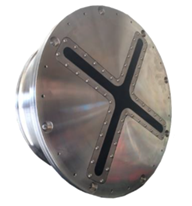
\includegraphics[width=\linewidth]{gfx/chapter-detection/sonar/Sonar_antennas.png}
  \end{minipage}
  \hspace{1cm}
  \begin{minipage}{0.4\linewidth}
    \centering
    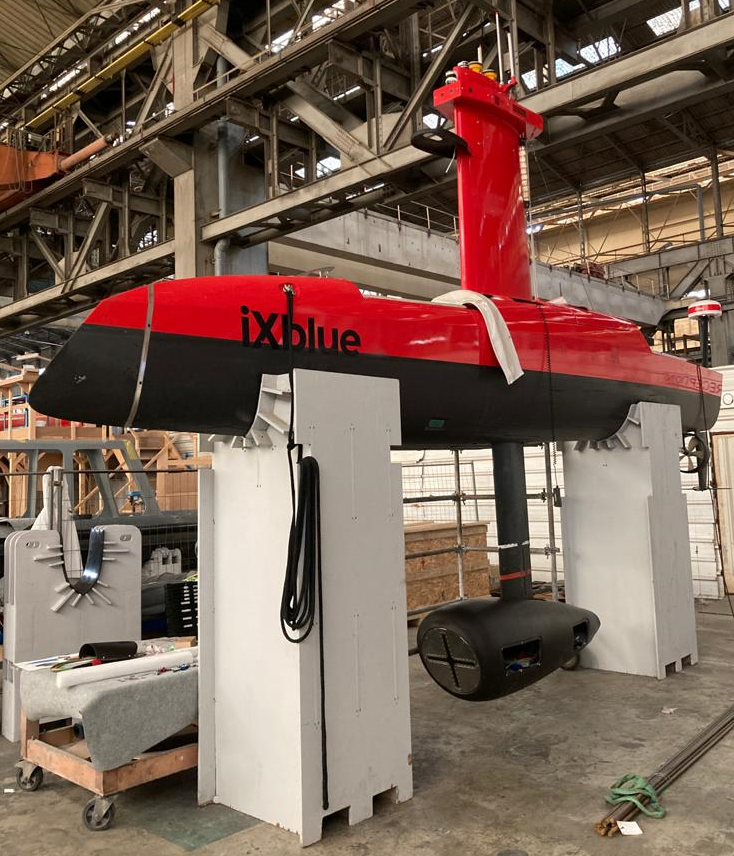
\includegraphics[width=\linewidth]{gfx/chapter-detection/sonar/SPX_and_DriX.png}
  \end{minipage}
  \caption{À gauche: face active du SEAPIX, les deux antennes linéaires de 64 capteurs se croisent en leur centre. À droite: le sonar installé dans la gondole du drone de surface DriX, en configuration de sonar frontal. Figures reprises de \cite{JOE24}.}
  \label{fig:detection-mills-systeme}
\end{figure}

Dans le cadre de la thèse, le SEAPIX est utilisé comme sonar frontal (\emph{forward-looking sonar}, FLS) à bord du drone de surface DriX, la face active orientée vers l'avant et inclinée de $20^\circ$. L'antenne verticale émet un faisceau large de $9^\circ$ en élévation par $120^\circ$ en azimut, puis les deux antennes reçoivent simultanément: l'antenne horizontale forme des voies en azimut et l'antenne verticale des voies en élévation. Les données utilisées ont été acquises en baie de La Ciotat en 2021 et 2022, par 50~m de fond, avec une sphère métallique de 71~cm immergée à 25~m comme cible de référence.

Le problème posé est alors celui de la \cref{def:detection-archetype-cible}: détecter une cible ponctuelle dans la réverbération du milieu. Deux constats sur les données réelles orientent le travail. D'une part, la réverbération n'est pas gaussienne: sur les premières centaines de mètres, la distribution de l'amplitude est proche d'une loi K de paramètre de forme $\nu\simeq3$, et elle ne redevient proche d'une loi normale qu'en fin de portée, là où le bruit ambiant domine \cite{JOE24}. Le modèle msg de la \cref{def:detection-msg} et les détecteurs robustes de la \cref{subsec:detection radar} sont donc le bon point de départ. D'autre part, on dispose de deux antennes qui observent la même scène, et il est naturel de se demander ce que l'on gagne à les traiter conjointement.

\subsection{Modèle de données à deux antennes}
\label{subsec:detection-mills-modele}

Considérons d'abord chaque antenne séparément. Après formation des données en bande de base et compression d'impulsion, l'antenne $\iarray\in\{1,2\}$ fournit à chaque case distance un vecteur $\x_\iarray\in\C^{\Nsensor}$, et une cible ponctuelle vue dans la direction $\doa_\iarray$ s'écrit $\x_\iarray=\amplitude_\iarray\steering_\iarray+\z_\iarray$, avec $\steering_\iarray=\steering(\doa_\iarray)$ le vecteur directionnel de l'antenne. C'est exactement le problème de la \cref{def:detection-archetype-cible}, et l'on peut appliquer sur chaque antenne l'\detname{anmf} construit sur l'estimateur de Tyler \cref{eq:detection-anmf-tyler}. C'est ce qui est fait en pratique sur ce type de système, et c'est la référence à laquelle nous nous comparerons.

Ce traitement antenne par antenne a toutefois un défaut, lié à la corrélation de la réverbération. Chaque antenne présente une zone de moindre détectabilité autour de $0^\circ$ dans sa propre direction, et comme elle ne voit rien de l'autre direction, cette zone s'étend à toute une bande de l'espace: une bande verticale pour l'antenne horizontale, une bande horizontale pour l'antenne verticale. En combinant les deux antennes, une cible n'est aveugle que si elle est mal placée pour les deux à la fois. Pour exploiter cette complémentarité, on concatène les observations:

\begin{definition}[{Modèle à deux antennes}]
\label{def:detection-mills-modele}
  Notons $\x_\iarray\in\C^{\Nsensor}$ le vecteur reçu par l'antenne $\iarray\in\intrange{1}{\Narray}$, avec $\Narray=2$, et
  \begin{equation}
    \x = \begin{bmatrix}\x_1\\\x_2\end{bmatrix}\in\C^{\Narray\Nsensor},
    \qquad
    \Steermat = \begin{bmatrix}\steering_1 & \vector{0}\\\vector{0} & \steering_2\end{bmatrix}\in\C^{\Narray\Nsensor\times\Narray},
    \qquad
    \Vamplitude = \begin{bmatrix}\amplitude_1\\\amplitude_2\end{bmatrix}\in\C^{\Narray}.
    \label{eq:detection-mills-concat}
  \end{equation}
  Le problème de détection prend alors la forme de la \cref{def:detection-archetype-cible} avec $\Steermat\Vamplitude$ pour réponse cible:
  \begin{equation}
    \left\{
    \begin{array}{lll}
      \hypothesis_0: & \x = \z, & \x_\iobs = \z_\iobs, \quad \iobs\in\intrange{1}{\Nobs} \\[2pt]
      \hypothesis_1: & \x = \Steermat\Vamplitude + \z, \qquad & \x_\iobs = \z_\iobs, \quad \iobs\in\intrange{1}{\Nobs}.
    \end{array}
    \right.
    \label{eq:detection-mills-test}
  \end{equation}
\end{definition}

Les amplitudes $\amplitude_1$ et $\amplitude_2$ sont laissées libres, puisque les deux antennes n'ont ni la même ouverture ni le même gain. Reste à décrire le bruit $\z$. Dans la littérature radar, les détecteurs multi-antennes existants supposent soit un fouillis gaussien homogène sur toutes les antennes \sidecite{Chong201004}, soit des antennes non corrélées entre elles \cite{Chong201003}. Aucune de ces deux hypothèses ne convient ici. Les deux antennes n'observent pas la même portion de fond et leurs réverbérations n'ont pas de raison de fluctuer ensemble, mais elles partagent leur capteur central, si bien que les blocs d'intercorrélation ne sont pas nuls. La \cref{fig:detection-mills-covariance} le montre sur une scm estimée sur données réelles. D'où le modèle suivant:

\begin{definition}[{Modèle multi-textures}]
\label{def:detection-mills-multitexture}
  Chaque antenne porte sa propre texture et son propre facteur d'échelle. En posant $\escale_\iarray = \powerscale_\iarray\sqrt{\texture_\iarray}$ et
  \begin{equation}
    \Scalemat = \Diag\left(\escale_1,\escale_2\right)\otimes\Id{\Nsensor},
    \qquad
    \MScatter = \begin{bmatrix}\MScatter_{11} & \MScatter_{12}\\\MScatter_{21} & \MScatter_{22}\end{bmatrix},
    \label{eq:detection-mills-scalemat}
  \end{equation}
  la dispersion de l'observation vaut
  \begin{equation}
    \MCov = \Scalemat\,\MScatter\,\Scalemat,
    \label{eq:detection-mills-cov}
  \end{equation}
  où $\MScatter_{\iarray\iarray}$ est le bloc propre à l'antenne $\iarray$ et $\MScatter_{12}=\MScatter_{21}^\herm$ le bloc d'intercorrélation. Conditionnellement aux textures, les densités sous les deux hypothèses s'écrivent
  \begin{equation}
    \ddp{\x}(\x;\hypothesis_0) = \frac{\exp\left(-\quadraticH{\x}{\MCov}\right)}{\pi^{\Narray\Nsensor}\Det(\MCov)},
    \qquad
    \ddp{\x}(\x;\hypothesis_1) = \frac{\exp\left(-(\x-\Steermat\Vamplitude)^\herm\inv{\MCov}(\x-\Steermat\Vamplitude)\right)}{\pi^{\Narray\Nsensor}\Det(\MCov)}.
    \label{eq:detection-mills-pdf}
  \end{equation}
\end{definition}

\begin{figure}[htbp]
  \centering
  \begin{minipage}{0.45\linewidth}
    \includegraphics[width=\linewidth]{gfx/chapter-detection/sonar/SCM_example.pdf}
  \end{minipage}
  \begin{minipage}{0.45\linewidth}
    \includegraphics[width=\linewidth]{gfx/chapter-detection/sonar/Covariance_model.pdf}
  \end{minipage}
  \caption{À gauche: scm estimée sur données réelles SEAPIX dans une zone homogène entre 265~m et 328~m (en dB). Les blocs diagonaux correspondent à chaque antenne, les blocs hors diagonale à leur intercorrélation, qui n'est pas nulle. À droite: le modèle de covariance utilisé en simulation, $[\MScatter]_{jl}=\beta\rho_1^{\abs{j_1-l_1}}\rho_2^{\abs{j_2-l_2}}$ avec $\beta=3\times10^{-4}$, $\rho_1=0{,}4$ et $\rho_2=0{,}9$. Figures reprises de \cite{JOE24}.}
  \label{fig:detection-mills-covariance}
\end{figure}

\begin{remark}[{Ce que le modèle autorise}]
  Ce modèle permet de décrire deux antennes de statistiques différentes: on peut par exemple avoir une première antenne gaussienne ($\texture_1=1$) et homogène ($\powerscale_1=1$), et une seconde K-distribuée et partiellement homogène. Au sens de la \cref{def:detection-heterogeneite}, il s'agit d'une hétérogénéité \emph{par blocs}, intermédiaire entre le modèle usuel à une seule texture pour tout le vecteur et le cas où chaque capteur aurait la sienne, où plus rien ne serait identifiable. Le bloc $\MScatter_{12}$ est conservé, et c'est lui qui distingue ce modèle d'un traitement antenne par antenne.
\end{remark}

\subsection{Le trvg et l'apparition d'un terme croisé}
\label{subsec:detection-mills-tests}

Suivons la démarche en deux étapes de la \cref{subsec:detection radar}: on suppose d'abord $\MScatter$ connue, on dérive le test, puis on remplace $\MScatter$ par une estimée. À $\MScatter$ connue, les paramètres inconnus sont les amplitudes $\Vamplitude$ et les deux échelles $\escale_1,\escale_2$. Le trvg s'obtient en maximisant la vraisemblance en ces paramètres sous chaque hypothèse, et on obtient le résultat suivant \cite{JOE24}:

\begin{proposition}[{trvg à deux textures}]
\label{prop:detection-mills-glrt}
  Le trvg du problème \cref{eq:detection-mills-test} à $\MScatter$ connue s'écrit comme le quotient des échelles estimées sous chaque hypothèse:
  \begin{equation}
    \statGLRT(\x)
    =
    \frac{\hat{\escale}_{1,0}\,\hat{\escale}_{2,0}}{\hat{\escale}_{1,1}\,\hat{\escale}_{2,1}}
    \detect,
    \label{eq:detection-mills-glrt}
  \end{equation}
  où, en notant $\left[\inv{\MScatter}\right]_{\iarray\ivarbis}$ le bloc $(\iarray,\ivarbis)$ de $\inv{\MScatter}$,
  \begin{equation}
    \left(\hat{\escale}_{1,0}\,\hat{\escale}_{2,0}\right)^2
    =
    \frac{\Realp\left(\x_1^\herm\left[\inv{\MScatter}\right]_{12}\x_2\right)}{\Nsensor}
    +
    \sqrt{
      \frac{\x_1^\herm\left[\inv{\MScatter}\right]_{11}\x_1}{\Nsensor}
      \cdot
      \frac{\x_2^\herm\left[\inv{\MScatter}\right]_{22}\x_2}{\Nsensor}
    },
    \label{eq:detection-mills-sigma0}
  \end{equation}
  et où $\left(\hat{\escale}_{1,1}\,\hat{\escale}_{2,1}\right)^2$ est donnée par la même expression en substituant $\inv{\MScatter}-\projspace{\MScatter}$ à $\inv{\MScatter}$, avec
  \begin{equation}
    \projspace{\MScatter}
    =
    \inv{\MScatter}\Steermat\left(\Steermat^\herm\inv{\MScatter}\Steermat\right)^{-1}\Steermat^\herm\inv{\MScatter}.
    \label{eq:detection-mills-projecteur}
  \end{equation}
\end{proposition}

Le détecteur est donc un rapport des puissances résiduelles estimées sans et avec la cible, comme le \detname{nmf} en mono-antenne. La nouveauté est dans \cref{eq:detection-mills-sigma0}: en plus des deux formes quadratiques propres à chaque antenne apparaît le terme croisé $\Realp(\x_1^\herm[\inv{\MScatter}]_{12}\x_2)$, qui fait intervenir la corrélation entre les deux antennes dans l'estimation de leurs échelles. C'est ce terme qui permet de situer le détecteur par rapport à ceux de la littérature:
\begin{itemize}
  \item pour une seule antenne, \cref{eq:detection-mills-glrt} se ramène, à une transformation monotone près, au \detname{nmf} \cref{eq:detection-nmf};
  \item lorsque les antennes sont décorrélées, $[\inv{\MScatter}]_{12}=\mat{0}$, le terme croisé disparaît et l'on retrouve le détecteur \textsc{mimo} de \citet{Chong201003}, c'est-à-dire un produit de deux \detname{nmf};
  \item lorsque les deux échelles sont égales, on retrouve la version par sous-espace de l'\textsc{ace} \cite{Raghavan2016}.
\end{itemize}
Le trvg à deux textures est donc une généralisation bi-antenne du \detname{nmf}, que l'on notera \detname{m-nmf-g}, et sa version adaptative une généralisation de l'\detname{anmf}.

\begin{property}[{Invariance aux textures}]
\label{prop:detection-mills-cfar}
  La statistique \cref{eq:detection-mills-glrt} est texture-cfar au sens de la \cref{def:detection-cfar}: sa loi sous $\hypothesis_0$ ne dépend ni de $\texture_1$ ni de $\texture_2$.
\end{property}

\subsection{Pourquoi passer au test de Rao}
\label{subsec:detection-mills-rao}

Le trvg \cref{eq:detection-mills-glrt} présente deux inconvénients pratiques. Le premier est son coût: les échelles sous $\hypothesis_1$ font intervenir le projecteur $\projspace{\MScatter}$, qui dépend de la direction testée $(\doa_1,\doa_2)$. Il faut donc les recalculer pour chaque couple de directions, alors que le balayage porte sur $64\times64$ couples par case distance. Le second est sa loi: si l'on dispose d'une relation $\pfa$-seuil exacte à $\MScatter$ connue, les simulations montrent que la version adaptative n'est plus matrice-cfar lorsque la fausse alarme visée est faible \cite{JOE24}, ce qui empêche de fixer un seuil une fois pour toutes.

Le test de Rao répond aux deux. Il ne demande l'estimation des paramètres de nuisance que sous $\hypothesis_0$, et sous $\hypothesis_0$ les échelles estimées \cref{eq:detection-mills-sigma0} ne dépendent pas de $\Steermat$: une seule estimation par case distance sert à tout le balayage angulaire. En écrivant le problème sous la forme \cref{eq:detection-test-parametre} avec $\paramtest=[\Realp(\Vamplitude)^\T,\operatorname{Im}(\Vamplitude)^\T]^\T\in\R^4$ et $\paramnuis=[\escale_1,\escale_2]^\T$, on obtient \sidecite{GRETSI23a}:

\begin{proposition}[{Test de Rao à deux textures}]
\label{prop:detection-mills-rao}
  Le test de Rao du problème \cref{eq:detection-mills-test} s'écrit comme une énergie projetée:
  \begin{equation}
    \statRao(\x)
    =
    2\,\x^\herm\inv{\widehat{\MCov}_0}\Steermat
    \left(\Steermat^\herm\inv{\widehat{\MCov}_0}\Steermat\right)^{-1}
    \Steermat^\herm\inv{\widehat{\MCov}_0}\,\x
    \detect,
    \label{eq:detection-mills-rao}
  \end{equation}
  où $\widehat{\MCov}_0 = \widehat{\Scalemat}_0\,\MScatter\,\widehat{\Scalemat}_0$, les échelles de $\widehat{\Scalemat}_0$ valant
  \begin{equation}
    \hat{\escale}_{1,0}^2 = s_1 + \sqrt{\frac{s_1}{s_2}}\,s_{12},
    \qquad
    \hat{\escale}_{2,0}^2 = s_2 + \sqrt{\frac{s_2}{s_1}}\,s_{12},
    \label{eq:detection-mills-echelles-h0}
  \end{equation}
  avec $s_\iarray = \x_\iarray^\herm[\inv{\MScatter}]_{\iarray\iarray}\x_\iarray/\Nsensor$ et $s_{12}=\Realp(\x_1^\herm[\inv{\MScatter}]_{12}\x_2)/\Nsensor$.
\end{proposition}

On reconnaît dans \cref{eq:detection-mills-rao} le filtre adapté \textsc{mimo} de \sidecite{Chong201004}, qui est le détecteur optimal en fouillis gaussien homogène à covariance connue, évalué ici en une covariance dont les échelles de chaque antenne ont été estimées sur l'observation elle-même. On retrouve aussi le terme croisé $s_{12}$, cette fois dans l'estimation des échelles. Le test est texture-cfar, et sa forme d'énergie projetée donne directement sa loi sous $\hypothesis_0$:

\begin{proposition}[{Relation $\pfa$-seuil du test de Rao}]
\label{prop:detection-mills-rao-pfa}
  Sous $\hypothesis_0$, $\statRao$ suit asymptotiquement (en $\Nsensor$) une loi du $\chisquared$ à quatre degrés de liberté, d'où
  \begin{equation}
    \pfa = \exp\left(-\frac{\DetectorTreshold}{2}\right)\left(1+\frac{\DetectorTreshold}{2}\right),
    \label{eq:detection-mills-rao-pfa}
  \end{equation}
  qui ne dépend ni des textures ni de $\MScatter$.
\end{proposition}

En simulation, le régime asymptotique est atteint dès $\Nsensor=64$, ce qui est le cas du SEAPIX, et la relation \cref{eq:detection-mills-rao-pfa} reste vérifiée en version adaptative pour des matrices de covariance très différentes \cite{JOE24}. C'est la raison principale pour laquelle nous privilégions le test de Rao, que l'on notera \detname{m-nmf-r}.

\begin{remark}[{Pourquoi le test de Rao}]
\label{rem:detection-pourquoi-rao}
  Le test de Rao est souvent présenté comme une approximation du trvg, plus simple à calculer. Ici, il présente trois avantages qui dépassent la simplicité de calcul. D'abord, l'estimée sous $\hypothesis_0$ ne dépend pas de la direction testée, ce qui rend le balayage angulaire peu coûteux. Ensuite, sa loi sous $\hypothesis_0$ est connue en forme close et ne dépend pas de la covariance pour $\Nsensor$ grand, ce qui permet de régler le seuil sans simulation. Enfin, comme il est construit au voisinage de $\hypothesis_0$, il ne cherche pas à expliquer l'observation par un signal quelconque, et il est plus sélectif vis-à-vis des signaux qui ne correspondent pas à la direction testée. Ce dernier point sera mis en regard, en \cref{sec:detection-fls}, du choix inverse que font les détecteurs par sous-espaces.
\end{remark}

\subsection{Estimation robuste sous textures multiples}
\label{subsec:detection-mills-estimation}

Reste la seconde étape: remplacer $\MScatter$ par une estimée issue de $\Nobs$ données secondaires. En fouillis gaussien, la scm convient, mais en fouillis msg elle est dominée par les données de forte puissance. Il faut donc un estimateur de Tyler adapté au modèle à deux textures. En maximisant la vraisemblance des données secondaires sous le modèle de la \cref{def:detection-mills-multitexture}, on obtient \sidecite{JOE24}:

\begin{proposition}[{Estimateur de Tyler à deux textures}]
\label{prop:detection-mills-tyler}
  Sous le modèle de la \cref{def:detection-mills-multitexture}, l'estimateur du maximum de vraisemblance de $\MScatter$ vérifie
  \begin{equation}
    \widehat{\MScatter}
    =
    \frac{1}{\Nobs}\sum_{\iobs=1}^{\Nobs}
    \inv{\widehat{\mat{T}}_\iobs}\,\x_\iobs\x_\iobs^\herm\,\inv{\widehat{\mat{T}}_\iobs},
    \qquad
    \widehat{\mat{T}}_\iobs = \Diag\left(\sqrt{\hat{\texture}_{1,\iobs}},\sqrt{\hat{\texture}_{2,\iobs}}\right)\otimes\Id{\Nsensor},
    \label{eq:detection-mills-tyler}
  \end{equation}
  où les textures $\hat{\texture}_{1,\iobs}$ et $\hat{\texture}_{2,\iobs}$ sont données par \cref{eq:detection-mills-echelles-h0} appliquée à $\x_\iobs$ et à $\widehat{\MScatter}$.
\end{proposition}

On retrouve la structure de l'estimateur de Tyler (\cref{def:context-complex-tyler}): chaque donnée est normalisée par sa propre puissance avant d'être moyennée, ce qui rend l'estimée indépendante des textures. La différence est que la normalisation se fait par bloc, et que la texture d'une antenne est estimée en tenant compte, à travers le terme croisé, de ce qu'observe l'autre. L'estimateur se calcule par un algorithme de point fixe, dont la convergence est rapide en pratique\footnote{L'existence et l'unicité de la solution ne sont en revanche pas établies. Voir l'annexe~D de l'article reproduit p.~\paperpage{JOE24} pour la dérivation et l'algorithme.}. En remplaçant $\MScatter$ par $\widehat{\MScatter}$ dans \cref{eq:detection-mills-glrt,eq:detection-mills-rao}, on obtient les versions adaptatives des deux détecteurs.

\subsection{Ce que la fusion des antennes apporte}
\label{subsec:detection-mills-perf}

Les simulations de \cite{JOE24} utilisent le modèle de covariance de la \cref{fig:detection-mills-covariance}, $\Nobs=2\times2\Nsensor=256$ données secondaires et $\pfa=10^{-2}$. On peut en retenir les éléments suivants:
\begin{itemize}
  \item à covariance connue, en fouillis gaussien, les détecteurs bi-antennes gagnent environ 2,5~dB et 2~dB par rapport aux \detname{nmf} de chacune des antennes, à $\pdet=0{,}8$, et ne sont qu'à 0,2~dB du filtre adapté \textsc{mimo} qui connaît toute la covariance;
  \item le gain se lit surtout dans le plan azimut-élévation: là où l'antenne horizontale seule a une probabilité de détection de 0,17 sur toute la bande $\doa_1=0^\circ$, et l'antenne verticale 0,03 sur la bande $\doa_2=0^\circ$, le test de Rao dépasse 0,8 dès que $\abs{\doa_2}>10{,}5^\circ$. La zone aveugle se réduit à un voisinage du centre;
  \item en fouillis gaussien partiellement homogène, le filtre adapté \textsc{mimo} adaptatif ne contrôle plus la fausse alarme et devient moins bon que l'\detname{anmf} mono-antenne, alors que les détecteurs proposés ne sont pas affectés, étant invariants aux échelles;
  \item en fouillis K-distribué ($\nu=0{,}5$), l'estimateur à deux textures apporte environ 1,2~dB par rapport à la scm, et 3~dB par rapport au meilleur des détecteurs concurrents.
\end{itemize}

% ============================== FIGURE 4/9 =========================================
% ATTENTION: RUN DEBUG (n_h0 = n_h1 = 200, 12 points de rsb au lieu de 150).
% Version definitive:
%   uv run qanat experiment run sonar_pd_snr --n-trials-h0 10000 --n-trials-h1 10000
% puis --k-dist pour le second panneau. La provenance porte debug=True tant que
% ce n'est pas fait.
%
% TODO: cette figure n'a pour l'instant que le cas gaussien. Le plan en demande
% deux, gaussien et K-distribue (nu = 0.5), cote a cote --- c'est la comparaison
% qui porte l'argument (la robustesse coute peu sous modele gaussien et rapporte
% beaucoup sinon). Relancer avec --k-dist et enregistrer sous l'id pd-rsb-k.
%
% TODO decision: le MATLAB de reference trace chaque famille de courbes sur SON
% propre axe de rsb (snrP pour l'antenne 1, snrA pour l'antenne 2, snrPA pour le
% bi-antenne), ce que l'article ne dit nulle part. Ici tout est sur un axe
% commun, d'ou l'ecart mono-antenne 1 / mono-antenne 2 plus marque que dans
% l'article. A trancher: axe commun (honnete mais different de l'article) ou
% convention de l'article (comparable mais a expliquer en note).
% ====================================================================================
\begin{figure}[htbp]
  \centering
  % This file was created with matplot2tikz v0.5.3.
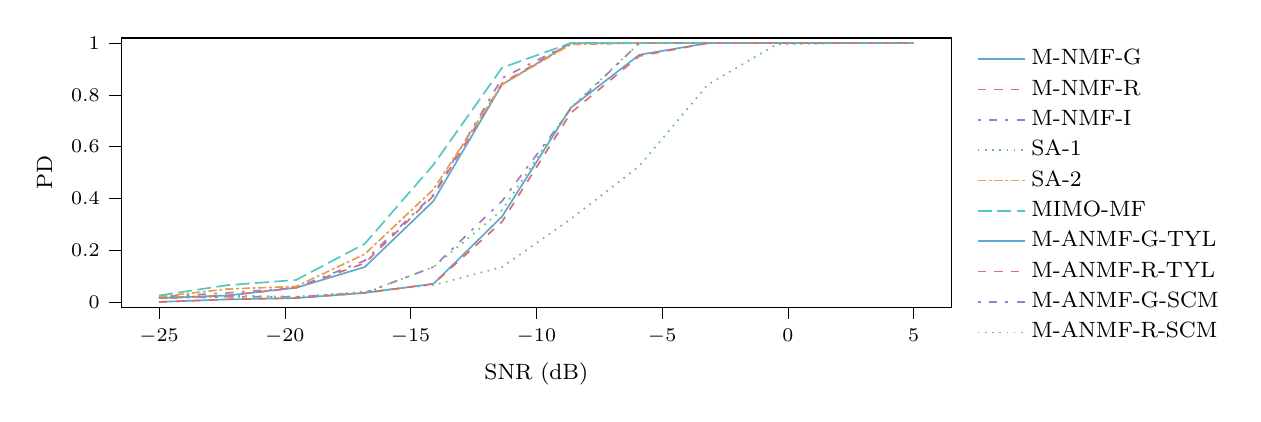
\begin{tikzpicture}

\definecolor{cornflowerblue92168211}{RGB}{92,168,211}
\definecolor{darkgray176}{RGB}{176,176,176}
\definecolor{indianred224107107}{RGB}{224,107,107}
\definecolor{mediumpurple165123197}{RGB}{165,123,197}
\definecolor{mediumseagreen107191107}{RGB}{107,191,107}
\definecolor{mediumturquoise80200192}{RGB}{80,200,192}
\definecolor{sandybrown22416080}{RGB}{224,160,80}

\begin{axis}[
height=5cm,
label style={font=\footnotesize},
legend cell align={left},
legend style={
  fill opacity=0.8,
  draw opacity=1,
  text opacity=1,
  at={(1.02,1)},
  anchor=north west,
  draw=none
},
legend style={draw=none, fill=white, fill opacity=0.9, text opacity=1, font=\footnotesize},
tick align=outside,
tick label style={font=\scriptsize},
tick pos=left,
title style={font=\footnotesize, yshift=-2pt},
width=\textwidth,
x grid style={darkgray176},
xlabel={SNR (dB)},
xmin=-26.5, xmax=6.5,
xtick style={color=black},
y grid style={darkgray176},
ylabel={PD},
ymin=-0.02, ymax=1.02,
ytick style={color=black}
]
\addplot [semithick, cornflowerblue92168211]
table {%
-25 0.015
-22.2727272727273 0.025
-19.5454545454545 0.055
-16.8181818181818 0.135
-14.0909090909091 0.39
-11.3636363636364 0.84
-8.63636363636364 1
-5.90909090909091 1
-3.18181818181818 1
-0.454545454545457 1
2.27272727272727 1
5 1
};
\addlegendentry{M-NMF-G}
\addplot [semithick, indianred224107107, dashed]
table {%
-25 0.015
-22.2727272727273 0.025
-19.5454545454545 0.055
-16.8181818181818 0.15
-14.0909090909091 0.41
-11.3636363636364 0.845
-8.63636363636364 1
-5.90909090909091 1
-3.18181818181818 1
-0.454545454545457 1
2.27272727272727 1
5 1
};
\addlegendentry{M-NMF-R}
\addplot [semithick, mediumpurple165123197, dash pattern=on 1pt off 3pt on 3pt off 3pt]
table {%
-25 0.02
-22.2727272727273 0.035
-19.5454545454545 0.055
-16.8181818181818 0.16
-14.0909090909091 0.415
-11.3636363636364 0.865
-8.63636363636364 1
-5.90909090909091 1
-3.18181818181818 1
-0.454545454545457 1
2.27272727272727 1
5 1
};
\addlegendentry{M-NMF-I}
\addplot [semithick, mediumseagreen107191107, dotted]
table {%
-25 0.015
-22.2727272727273 0.025
-19.5454545454545 0.02
-16.8181818181818 0.04
-14.0909090909091 0.065
-11.3636363636364 0.135
-8.63636363636364 0.32
-5.90909090909091 0.525
-3.18181818181818 0.84
-0.454545454545457 0.995
2.27272727272727 1
5 1
};
\addlegendentry{SA-1}
\addplot [semithick, sandybrown22416080, dash pattern=on 3pt off 1pt on 1pt off 1pt]
table {%
-25 0.02
-22.2727272727273 0.05
-19.5454545454545 0.06
-16.8181818181818 0.185
-14.0909090909091 0.435
-11.3636363636364 0.84
-8.63636363636364 0.995
-5.90909090909091 1
-3.18181818181818 1
-0.454545454545457 1
2.27272727272727 1
5 1
};
\addlegendentry{SA-2}
\addplot [semithick, mediumturquoise80200192, dash pattern=on 5pt off 2pt]
table {%
-25 0.025
-22.2727272727273 0.065
-19.5454545454545 0.085
-16.8181818181818 0.225
-14.0909090909091 0.53
-11.3636363636364 0.905
-8.63636363636364 1
-5.90909090909091 1
-3.18181818181818 1
-0.454545454545457 1
2.27272727272727 1
5 1
};
\addlegendentry{MIMO-MF}
\addplot [semithick, cornflowerblue92168211]
table {%
-25 0
-22.2727272727273 0.01
-19.5454545454545 0.015
-16.8181818181818 0.035
-14.0909090909091 0.07
-11.3636363636364 0.33
-8.63636363636364 0.75
-5.90909090909091 0.955
-3.18181818181818 1
-0.454545454545457 1
2.27272727272727 1
5 1
};
\addlegendentry{M-ANMF-G-TYL}
\addplot [semithick, indianred224107107, dashed]
table {%
-25 0
-22.2727272727273 0.01
-19.5454545454545 0.015
-16.8181818181818 0.035
-14.0909090909091 0.07
-11.3636363636364 0.31
-8.63636363636364 0.73
-5.90909090909091 0.95
-3.18181818181818 1
-0.454545454545457 1
2.27272727272727 1
5 1
};
\addlegendentry{M-ANMF-R-TYL}
\addplot [semithick, mediumpurple165123197, dash pattern=on 1pt off 3pt on 3pt off 3pt]
table {%
-25 0.015
-22.2727272727273 0.02
-19.5454545454545 0.02
-16.8181818181818 0.035
-14.0909090909091 0.135
-11.3636363636364 0.39
-8.63636363636364 0.745
-5.90909090909091 1
-3.18181818181818 1
-0.454545454545457 1
2.27272727272727 1
5 1
};
\addlegendentry{M-ANMF-G-SCM}
\addplot [semithick, mediumseagreen107191107, dotted]
table {%
-25 0.015
-22.2727272727273 0.02
-19.5454545454545 0.02
-16.8181818181818 0.035
-14.0909090909091 0.135
-11.3636363636364 0.355
-8.63636363636364 0.75
-5.90909090909091 1
-3.18181818181818 1
-0.454545454545457 1
2.27272727272727 1
5 1
};
\addlegendentry{M-ANMF-R-SCM}
\end{axis}

\end{tikzpicture}

  \provPdRsbQR[1cm]
  \caption{$\pdet$ en fonction du rapport signal à bruit, à $\pfa=10^{-2}$, en
  fouillis gaussien ($m=64$, $\Nobs=256$, pointage $\theta_1=\theta_2=45^\circ$).
  Le filtre adapte mimo à dispersion connue borne les performances; les tests
  glrt et de Rao à dispersion connue s'en approchent à quelques dixiemes de dB,
  et leurs versions adaptatives paient l'estimation. Les detecteurs
  mono-antenne restent en retrait: c'est le gain de la fusion des deux
  antennes. \provPdRsb}
  \label{fig:detection-mills-pd-rsb}
\end{figure}

\wipfig{FIGURE 3/9}{Carte $\pdet(\doa_1,\doa_2)$ pour \detname{nmf} 1, \detname{nmf} 2 et le test de Rao à covariance connue, RSB $=-12$~dB. Expérience: sonar\_pd\_angle.}

Sur données réelles, la cible de référence est correctement localisée en azimut et en élévation par les deux détecteurs. L'intérêt de l'estimateur robuste apparaît lorsque les données secondaires sont contaminées: en ajoutant une cible synthétique à 100 cases distance de la cible réelle, le test de Rao construit sur la scm ne permet plus de distinguer la cible et place son maximum au mauvais endroit, alors que la version construite sur l'estimateur à deux textures reste exploitable (\cref{fig:detection-mills-contamination}).

\begin{figure}[htbp]
  \centering
  \includegraphics[width=0.49\linewidth]{gfx/chapter-detection/sonar/M_ANMF_R_SCM_corrupted_output.pdf}
  \includegraphics[width=0.49\linewidth]{gfx/chapter-detection/sonar/M_ANMF_R_TYL_corrupted_output.pdf}
  \caption{Sortie du test de Rao adaptatif sur données réelles SEAPIX lorsque les données secondaires sont contaminées par une seconde cible. À gauche avec la scm, à droite avec l'estimateur à deux textures \cref{eq:detection-mills-tyler}, tous deux sur 256 données secondaires. Figures reprises de \cite{JOE24}, les données n'étant pas diffusables.}
  \label{fig:detection-mills-contamination}
\end{figure}

\section{Détection multi-pings et sous-espaces pour un sonar frontal}
\label{sec:detection-fls}

\begin{contributions}
  Cette section reprend \fullcite{JOE26}.
\end{contributions}

% ============================ TODO texte (~2 paragraphes) ==========================
% Transition depuis la section precedente, puis contexte:
%  - on y exploitait une structure *entre antennes*; on exploite ici une
%    structure *entre pings* successifs, c'est-a-dire une integration coherente
%    dans le temps --- l'analogue sonar du traitement espace-temps (stap) du
%    radar;
%  - le gain attendu: sommer en phase $\Nping$ echos ameliore le rapport signal
%    a bruit; le prix a payer: la dimension du probleme est multipliee par
%    $\Nping$, et le nombre de donnees secondaires necessaires avec elle. C'est
%    exactement le probleme annonce en fin de \cref{sec:detection-cadre};
%  - second prix a payer, moins evident et c'est le fil de la section: sommer
%    en phase suppose de connaitre la phase. Toute erreur de recalage degrade
%    la detection, d'ou la seconde moitie de la section sur les sous-espaces.
% ====================================================================================

\subsection{Modèle multi-pings}
\label{subsec:detection-fls-modele}

\begin{definition}[{Modèle multi-pings}]
\label{def:detection-fls-modele}
  Après recalage, la concaténation des $\Nping$ pings s'écrit $\x = [\x_1^\T\ \cdots\ \x_{\Nping}^\T]^\T\in\C^{\Nsensor\Nping}$ et la réponse d'une cible ponctuelle vue dans la direction $\doa$ vaut
  \begin{equation}
    \x = \amplitude\,\steerfull(\doa) + \z,
    \qquad
    \steerfull(\doa) = \vector{1}_{\Nping}\otimes\steering(\doa),
    \label{eq:detection-fls-modele}
  \end{equation}
  où $\vector{1}_{\Nping}\in\R^{\Nping}$ est le vecteur de composantes unité et $\steering(\doa)\in\C^{\Nsensor}$ le vecteur directionnel d'un ping.
\end{definition}

% ======================= TODO texte (remarque, ~5 lignes) ==========================
% Lire la decomposition de Kronecker de \cref{eq:detection-fls-modele}, elle
% structure toute la section: l'operande de gauche est *interferometrique* (il
% somme en phase les echos ping a ping), celui de droite est purement
% *angulaire* (il somme en phase les capteurs dans la direction $\doa$). Le
% vecteur $\vector{1}_{\Nping}$ suppose un recalage parfait --- hypothese que
% la \cref{subsec:detection-fls-sousespace} viendra relacher, et c'est
% precisement sur cet operande de gauche que portera le sous-espace.
% Renvoyer au pdf joint pour la chaine de recalage elle-meme, qui n'est pas
% reprise ici.
% ====================================================================================

\subsection{Structure de Kronecker de la dispersion du fouillis}
\label{subsec:detection-fls-kronecker}

\begin{proposition}[{Structure de la dispersion du fouillis}]
\label{prop:detection-fls-kronecker}
  En modélisant le fouillis comme la somme des contributions indépendantes de $N_c$ facettes insonifiées, de réponses $\z_n = \amplitude_n\,\vector{1}_{\Nping}\otimes\steering(\doa_n)$ avec $\E\{\amplitude_\ivar\conj{\amplitude_\ivarbis}\}=0$ pour $\ivar\neq\ivarbis$, la dispersion du fouillis vaut
  \begin{equation}
    \MScatter_c
    =
    \sum_{n=1}^{N_c}\E\left\{\abs{\amplitude_n}^2\right\}\,
    \vector{1}_{\Nping}\vector{1}_{\Nping}^\herm
    \otimes
    \steering(\doa_n)\steering(\doa_n)^\herm.
    \label{eq:detection-fls-kronecker}
  \end{equation}
  Elle possède donc naturellement une structure de produit de Kronecker.
\end{proposition}

% ======================= TODO texte (remarque, ~5 lignes) ==========================
% Souligner que la structure est *derivee* et non postulee: elle decoule du
% modele physique de reverberation, alors que la litterature l'introduit le
% plus souvent comme une hypothese de commodite \sidecite{Wirfalt2014}.
% Ajouter que l'operande angulaire herite en outre d'une structure Toeplitz du
% fait de l'antenne lineaire uniforme, et qu'une ponderation des fluctuations
% de reflectivite ping a ping (intrinsic clutter motion, \sidecite{Lombardo2001})
% ne remet pas en cause la forme \cref{eq:detection-fls-kronecker}.
% ====================================================================================

\begin{proposition}[{Nombre de paramètres}]
\label{prop:detection-fls-comptage}
  Une dispersion hermitienne non structurée de taille $\Nsensor\Nping$ compte $(\Nsensor\Nping)^2$ paramètres réels. Sous la contrainte $\MScatter=\Kronleft\otimes\Kronright$ avec $\Kronleft\in\HPD{\Nping}$ et $\Kronright\in\HPD{\Nsensor}$ Toeplitz, ce nombre tombe à
  \begin{equation}
    \Nping^2 + 2\Nsensor - 1 - 1,
    \label{eq:detection-fls-comptage}
  \end{equation}
  le dernier terme retranchant l'indétermination d'échelle entre les deux opérandes.
\end{proposition}

% ======================= TODO texte (~4 lignes) --- CHIFFRE CLE ====================
% Faire l'application numerique, c'est l'argument qui justifie toute la
% section et il n'apparait pas dans l'article: pour $\Nsensor=64$ et
% $\Nping=5$, on passe de $102\,400$ a $151$ parametres reels, soit un facteur
% $\simeq 680$. Rapprocher ce chiffre de la regle $\Nobs\simeq2\vdim$ evoquee
% en \cref{sec:detection-cadre}: sans structure, il faudrait $\Nobs=640$
% donnees secondaires, soit environ 44 m de fond suppose homogene --- une
% hypothese que la scene ne verifie pas. C'est la que se joue le passage du
% principe a l'operationnel.
% ====================================================================================

\subsection{Estimation robuste structurée}
\label{subsec:detection-fls-estimation}

\begin{definition}[{Problème d'estimation structurée}]
\label{def:detection-fls-optim}
  En notant $\obsmat_\iobs$ la matrice telle que $\vecop(\obsmat_\iobs)=\x_\iobs$, l'estimation robuste sous contrainte de structure s'écrit \sidecite[-1cm]{sun2016robust}
  \begin{equation}
    \begin{array}{ll}
      \displaystyle\min_{\Kronleft,\,\Kronright\succ\vector{0}} & \loss\left(\Kronleft,\Kronright\right) \\[4pt]
      \text{sous contrainte} & \Kronright \in \Toep{\Nsensor}
    \end{array}
    \label{eq:detection-fls-optim}
  \end{equation}
  avec le critère de type Tyler
  \begin{equation}
    \loss\left(\Kronleft,\Kronright\right)
    =
    \Nsensor\ln\Det(\Kronleft)
    + \Nping\ln\Det(\Kronright)
    + \frac{\Nsensor\Nping}{\Nobs}\sum_{\iobs=1}^{\Nobs}
      \ln\trace{\Kronleft^{-\T}\obsmat_\iobs^\herm\inv{\Kronright}\obsmat_\iobs}.
    \label{eq:detection-fls-cout}
  \end{equation}
\end{definition}

% ======================= TODO texte (~3 lignes) ====================================
% Signaler la seule difference avec \sidecite{sun2016robust}: la transposee de
% $\inv{\Kronleft}$ dans la trace, qui est ce qui permet de traiter un operande
% $\Kronleft$ *complexe* et non reel. C'est un ajout modeste mais necessaire
% ici, l'operande interferometrique etant complexe par nature.
% ====================================================================================

\begin{proposition}[{Point fixe sur l'opérande interférométrique}]
\label{prop:detection-fls-A}
  À $\Kronright$ fixée, le minimiseur de \cref{eq:detection-fls-cout} sous la normalisation $\trace{\Kronleft}=1$ vérifie
  \begin{equation}
    \widehat{\Kronleft}
    =
    \frac{\Nping}{\Nobs}\sum_{\iobs=1}^{\Nobs}
    \frac{\left(\obsmat_\iobs^\herm\inv{\Kronright}\obsmat_\iobs\right)^\T}
         {\trace{\widehat{\Kronleft}^{-\T}\obsmat_\iobs^\herm\inv{\Kronright}\obsmat_\iobs}}.
    \label{eq:detection-fls-A}
  \end{equation}
\end{proposition}

\begin{proposition}[{Opérande angulaire Toeplitz}]
\label{prop:detection-fls-B}
  À $\Kronleft$ fixée, la contrainte Toeplitz se traite par plongement circulant: on écrit $\Kronright = \Unit\eigset\Unit^\herm$ avec $\Unit = \left[\Id{\Nsensor}\ \vector{0}_{\Nsensor,\Nsensor-1}\right]\mat{F}_{2\Nsensor-1}$, où $\mat{F}_{2\Nsensor-1}$ est la matrice de Fourier normalisée, de sorte que l'estimation de $\Kronright$ se ramène à celle des éléments diagonaux de $\eigset$, obtenus par l'itération de majoration-minimisation de l'\cref{alg:detection-fls-bcd}.
\end{proposition}

\begin{algorithm}[h]
\caption{Estimation robuste à structure Kronecker et Toeplitz}
\label{alg:detection-fls-bcd}
\begin{algorithmic}[1]
  \Require $\{\x_\iobs\}_{\iobs=1}^{\Nobs}$, $\Kronleft^{(0)}=\Id{\Nping}/\Nping$, $\eigset^{(0)}=\Id{2\Nsensor-1}$
  \While{convergence non atteinte}
    \State mettre à jour $\Kronleft$ par itération de \cref{eq:detection-fls-A} à $\Kronright$ fixée, puis normaliser par $\trace{\Kronleft}$
    \State $\vector{w} \gets \Diag\left(\Unit^\herm\inv{\Kronright}\Unit\right)$
    \State $\obsmat \gets \dfrac{\Nsensor}{\Nobs}\displaystyle\sum_{\iobs=1}^{\Nobs}\dfrac{\obsmat_\iobs\Kronleft^{-\T}\obsmat_\iobs^\herm}{\trace{\Kronleft^{-\T}\obsmat_\iobs^\herm\inv{\Kronright}\obsmat_\iobs}}$
    \State $\vector{d} \gets \Diag\left(\eigset\Unit^\herm\inv{\Kronright}\obsmat\inv{\Kronright}\Unit\eigset\right)$
    \State $\left[\vector{\eig}\right]_\ivar \gets \sqrt{\left[\vector{d}\right]_\ivar/\left[\vector{w}\right]_\ivar}$, \quad $\ivar\in\intrange{1}{2\Nsensor-1}$
    \State $\Kronright \gets \Unit\Diag\left(\vector{\eig}\right)\Unit^\herm$, puis normaliser par $\trace{\Kronright}$
  \EndWhile
  \Ensure $\widehat{\MScatter} = \Kronleft\otimes\Kronright$
\end{algorithmic}
\end{algorithm}

% ======================= TODO texte (remarque, ~6 lignes) ==========================
% Deux remarques a ecrire ici:
%  1. cas de l'antenne a element manquant: les deux antennes de la croix se
%     croisent en un capteur central qui ne peut appartenir aux deux, si bien
%     que l'antenne verticale est une ULA de 65 elements dont le central
%     manque. Le raisonnement reste valable a une matrice de permutation pres,
%     en modifiant $\Unit$ en consequence --- indispensable en pratique, faute
%     de quoi les resultats se degradent nettement. Le detail va dans le pdf
%     joint, une remarque suffit ici;
%  2. lien avec la partie 2, en pointeur et non en detour: le point fixe
%     \cref{eq:detection-fls-A} est une descente de gradient riemannienne sur
%     le cone (\cref{sec:context-riemann-optimization}), et c'est justement la
%     contrainte Toeplitz --- qui ne definit pas une sous-variete du cone
%     stable par l'exponentielle --- qui interdit d'y rester et impose le
%     detour par la majoration-minimisation.
% ====================================================================================

\subsection{Robustesse au désalignement: détection par sous-espace}
\label{subsec:detection-fls-sousespace}

\begin{definition}[{Sous-espace interférométrique}]
\label{def:detection-fls-sousespace}
  Soit $\Steerspace_{\Nrank}\in\C^{\Nsensor\Nping\times\Nrank}$, $\Nrank<\Nsensor\Nping$, de colonnes linéairement indépendantes, de la forme
  \begin{equation}
    \Steerspace_{\Nrank}
    =
    \mat{E}_{\Nrank}\otimes\steering(\doa),
    \qquad
    \left[\mat{E}_{\Nrank}\right]_{\iping\ivar}
    =
    \exp\left(-\frac{4\mathrm{j}\pi\,\xi_{\ivar,\iping}}{\wavelength}\right),
    \label{eq:detection-fls-sousespace}
  \end{equation}
  où les $\xi_{\ivar,\iping}$ sont des décalages de phase ping à ping. Le signal recherché est supposé appartenir au sous-espace engendré par les colonnes de $\Steerspace_{\Nrank}$, de coordonnées inconnues.
\end{definition}

\begin{proposition}[{Détecteur par sous-espace}]
\label{prop:detection-fls-anmf-sousespace}
  Le détecteur exploitant conjointement la structure de la dispersion et celle de la réponse cible s'écrit \sidecite[-1cm]{Kraut2001,Raghavan2016}
  \begin{equation}
    \DetectorStat_{\Nrank}(\x,\doa)
    =
    \frac{\abs{\hat{\steerfull}_{\Nrank}^\herm\inv{\widehat{\MScatter}}\x}^2}
         {\left(\hat{\steerfull}_{\Nrank}^\herm\inv{\widehat{\MScatter}}\hat{\steerfull}_{\Nrank}\right)
          \left(\x^\herm\inv{\widehat{\MScatter}}\x\right)}
    \detect,
    \label{eq:detection-fls-anmf-sousespace}
  \end{equation}
  où le signal estimé est la projection oblique de l'observation sur le sous-espace, dans la métrique induite par $\inv{\widehat{\MScatter}}$:
  \begin{equation}
    \hat{\steerfull}_{\Nrank}
    =
    \Steerspace_{\Nrank}
    \left(\Steerspace_{\Nrank}^\herm\inv{\widehat{\MScatter}}\Steerspace_{\Nrank}\right)^{-1}
    \Steerspace_{\Nrank}^\herm\inv{\widehat{\MScatter}}\,\x.
    \label{eq:detection-fls-projection}
  \end{equation}
\end{proposition}

% ================= TODO texte (remarque, ~8 lignes) --- POINT CLE ==================
% C'est le lien le plus fort entre les deux sections sonar, a ne pas manquer:
%  - la premiere colonne de $\mat{E}_{\Nrank}$ vaut $\vector{1}_{\Nping}$: on
%    retrouve exactement le modele \cref{eq:detection-fls-modele} d'une cible
%    parfaitement alignee en phase, et les colonnes suivantes ajoutent des
%    dephasages residuels;
%  - meme si le dephasage reel n'appartient pas exactement au sous-espace,
%    projeter sur $\Steerspace_{\Nrank}$ reduit l'angle de desadaptation par
%    rapport au cas $\Nrank=1$, d'ou le gain de robustesse;
%  - le rang $\Nrank$ est donc le curseur explicite de l'axe annonce en
%    \cref{rem:detection-pourquoi-rao}: chaque degre de liberte gagne en
%    robustesse au desalignement se paie par une perte sur cible parfaitement
%    alignee, puisque le detecteur accepte davantage de signaux;
%  - conclure que les deux sections sonar instrumentent ainsi le meme axe par
%    deux moyens opposes: le test de Rao en le parcourant vers le pole selectif,
%    le sous-espace en le parcourant vers le pole robuste.
% ====================================================================================

\subsection{Ce que la structure achète}
\label{subsec:detection-fls-perf}
% TODO decision: titre de sous-section a valider (cf. remarque analogue en
% \cref{subsec:detection-mills-perf}).

% ============================ TODO texte + figures =================================
\wipfig{FIGURE 7/9}{Pd vs RSB à N=32 et N=640, avec et sans Kronecker+Toeplitz. RIEN N'EXISTE côté qanat pour le volet FLS multi-pings. Traduit en performance le comptage 102 400 -> 151 paramètres pour m=64, P=5.}

% FIGURE 7/9 --- reproductible, A ECRIRE (rien n'existe cote qanat pour ce volet)
% $\pdet$ vs rapport signal a bruit a $\Nobs=32$ et $\Nobs=640$, avec et sans la
% structure Kronecker+Toeplitz. C'est la traduction en performance du comptage
% de la \cref{prop:detection-fls-comptage}: a $\Nobs=32$, le detecteur non
% structure est inutilisable et le detecteur structure fonctionne. Toute la
% section tient dans cette comparaison.
%
\wipfig{FIGURE 8/9}{Pd vs désadaptation de phase pour r dans {1,3,5}. RIEN N'EXISTE. CONTRAINTE FORTE: cette figure, la 7/9 et la 3/9 doivent partager axes, unités et Pfa --- c'est ce qui transforme l'axe sélectivité/robustesse d'une affirmation en une mesure.}

% FIGURE 8/9 --- reproductible, A ECRIRE
% $\pdet$ vs desadaptation de phase pour $\Nrank\in\{1,3,5\}$. Pendant exact de
% la figure angulaire de \cref{subsec:detection-mills-perf}: memes axes, memes
% unites, meme $\pfa$. Les deux figures lues ensemble donnent l'axe
% selectivite/robustesse en entier, du pole selectif (Rao) au pole robuste
% (sous-espace de rang eleve).
%
% Donnees reelles: sorties reprises de l'article \cite{JOE26}, non
% reproductibles (donnees non distribuables).
% ====================================================================================
\section{Détection de changements en-ligne pour les séries temporelles d'images RSO}
\label{sec:detection-online-change-detection}

\begin{contributions}
  Cette section reprend \fullcite{SP24}. Elle partage avec \fullcite{EUSIPCO21} la géométrie de la structure de Kronecker et le schéma d'estimation récursive, mais pas le modèle: les données y suivent une loi de Student, d'où un gradient et une borne différents.
\end{contributions}

La section précédente a montré qu'une structure de la matrice de covariance permet de réduire le nombre d'échantillons nécessaires à son estimation. Un problème commun à tous les détecteurs robustes vus jusqu'ici reste cependant entier: l'estimation passe par la résolution d'une équation de point fixe, dont le coût devient vite limitant lorsque l'on souhaite améliorer une estimation précédente en y ajoutant de nouvelles données. C'est précisément la situation de la détection de changements sur une série temporelle d'images RSO, où chaque nouvelle acquisition oblige à recalculer l'estimée sous $\hypothesis_0$ sur l'ensemble des dates. Dans ce contexte, la géométrie riemannienne permet de considérer un cadre d'estimation en ligne basé sur un algorithme de descente de gradient stochastique \cite{Zhou_2019}, pour lequel une seule itération suffit à chaque nouvelle image\sideref{sec:context-riemann-optimization}{Optimisation riemannienne}.

Ces travaux ont été menés avec Guillaume Ginolhac, Florent Bouchard et Arnaud Breloy. Ils combinent deux idées: supposer une structure de Kronecker pour la matrice de covariance, qui découle naturellement de la décomposition en ondelettes de \cite{Mian_wavelet_2019} appliquée aux canaux de polarisation, et mettre à jour récursivement l'estimée sous $\hypothesis_0$ par une descente de gradient naturel sur la variété des paramètres. Nous commençons par rappeler le problème et ses limitations pratiques, avant de détailler ces deux contributions puis de les illustrer sur données simulées et réelles.


\subsection{Problématique de la détection de changements sur matrices de covariances}

Commençons d'abord par introduire la problématique et les limitations pratiques des solutions proposées.

Nous considérons le traitement d'une série temporelle d'images RSO multivariée telle que présentée en Figure \ref{fig:example_its}. Dans ce contexte, chaque pixel correspond à un vecteur $\x\in\C^\vdim$, où $\vdim$ correspond usuellement à une diversité polarimétrique ($\vdim=3$ ou $\vdim=4$ selon les modalités) ou bien spectrale ou encore fréquentielle\footnote{\`A noter que dans la plupart des cas, on n'observe jamais une scène avec un capteur ayant une telle diversité mais avec une image de résolution suffisante, il est possible de constuire des images plus basses résolution ayant cette diversité \cite{Mian_wavelet_2019}.}.

\begin{figure*}
    \begin{tikzpicture}[scale=1]

% -------------------------------------------------
% parameters
% -------------------------------------------------
\pgfmathsetmacro{\cubex}{3}
\pgfmathsetmacro{\cubey}{2}
\pgfmathsetmacro{\cubez}{1}
\pgfmathsetmacro{\wf}{0.45}

% window size
\pgfmathsetmacro{\wx}{\wf*\cubex}
\pgfmathsetmacro{\wy}{\wf*\cubey}

% -------------------------------------------------
% cube drawing macro
% #1 = label index (1 or T)
% -------------------------------------------------
\newcommand{\DrawCube}[1]{

% ---- cube ----
\draw [every edge/.append style={densely dashed, opacity=.5}]
  (0,0,0) coordinate (o) -- ++(-\cubex,0,0) coordinate (a)
  -- ++(0,-\cubey,0) coordinate (b)
  edge coordinate[pos=1] (g) ++(0,0,-\cubez)
  -- ++(\cubex,0,0) coordinate (c) -- cycle
  (o) -- ++(0,0,-\cubez) coordinate (d)
  -- ++(0,-\cubey,0) coordinate (e)
  edge (g) -- (c) -- cycle
  (o) -- (a) -- ++(0,0,-\cubez) coordinate (f)
  edge (g) -- (d) -- cycle;

% ---- face center ----
\coordinate (Fc) at (-0.5*\cubex,-0.5*\cubey,0);

% window corners (robust)
\coordinate (W1) at ($(Fc)+(-\wx/2,\wy/2,0)$);
\coordinate (W2) at ($(Fc)+(\wx/2,-\wy/2,0)$);

% filled window
\fill[gray!20] (W1) rectangle (W2);

% 3x3 grid
% --- outer border ---
\draw (W1) rectangle (W2);

% --- vertical grid lines ---
\foreach \i in {1,2}{
  \draw ($(W1)+(\i*\wx/3,0,0)$) --
        ($(W1)+(\i*\wx/3,-\wy,0)$);
}

% --- horizontal grid lines ---
\foreach \i in {1,2}{
  \draw ($(W1)+(0,-\i*\wy/3,0)$) --
        ($(W1)+(\wx,-\i*\wy/3,0)$);
}


% annotation
\node[above=11pt] at (Fc) {$ \mathcal{X}_{\iobs #1}=\x_{\iobs #1}$};

% time label
\node at (-4,-1,0) {$t=#1$};

}

% -------------------------------------------------
% DRAW BOTH CUBES (HORIZONTAL)
% -------------------------------------------------

\foreach \label/\xshift in {1/0, T/7}{
  \begin{scope}[xshift=\xshift cm]
    \DrawCube{\label}
  \end{scope}
}

% vertical dots
\node at (-1.5,-2.25) {$\dots$};

\end{tikzpicture}


  \vspace{0.5em}
  \caption{Illustration de la dimensionalité de nos données SITS et de la fenêtre sur laquelle on considère les données pour le test de détection. $\x_{\iobs}$ est l'observation de la variable sous-jacente $\Variable_{\iobs\itime}$. }
  \label{fig:slidingwindows}
\end{figure*}



%TODO:: add figures of local neighborhood and global time series examples
%TODO: add citations
Pour effectuer une détection de changements, on se base sur la notion de voisinage spatial au cours du temps $\Xset_t = \{\x_{\iobs\itime}:1\leq \iobs \leq \Nobs\}$ comme illustré à la figure \ref{fig:slidingwindows}. En considérant que la distribution des données $\p{\Variable_{\iobs\itime}}$ est iid sur le voisinage : $\p{\Variable_{\iobs\itime}}(\x_{\iobs\itime})\equiv\p{\Variable_{t}}(\x_{\iobs\itime}),\,\forall \iobs\in\{1,\dots,\Nobs\}$, on peut identifier un changement à cet endroit à travers l'évolution de cette densité au cours du temps : si elle reste constante il n'y a pas eu de changements alors qu'une évolution de celle-ci indique qu'il s'est passé quelque chose. Formellement, on peut définir le problème de détection comme :



\begin{figure*}[p]
  \foreach \i in {1,...,16}{
    \includegraphics[width=0.3\textwidth]{gfx/chapter-detection/sar/sar_its/image_\i.jpg}
  }
  % TODO: find back the reference of image time series
  \caption{Exemple de SITS extraite de données UAVSAR polarimétriques en représentation de Pauli (Rouge: $|x_{\HH}-x_{\VV}|$, Rouge: $|x_{\HV}|$, Rouge: $|x_{\HH}+x_{\VV}|$). Images extraites à l'aide du code disponible à l'adresse: \url{https://github.com/AmmarMian/simulations_hdr/blob/main/2-detection/sar_experiments/visualisations/show_sar_its.py}.}
  \label{fig:example_its}
\end{figure*}

\begin{figure*}[t]
  % This file was created with matplot2tikz v0.5.3.
\begin{tikzpicture}

\definecolor{darkgray176}{RGB}{176,176,176}

\begin{axis}[
width=0.4\linewidth,
height=7cm,
colorbar,
colorbar style={ylabel={}},
colormap/viridis,
point meta max=248.592788696289,
point meta min=1.54258155822754,
tick align=outside,
tick pos=left,
title={$\DetectorStat_\gaussian$ (5.32s)},
x grid style={darkgray176},
xmin=-0.5, xmax=1493.5,
xtick style={color=black},
y dir=reverse,
y grid style={darkgray176},
ymin=-0.5, ymax=2993.5,
ytick style={color=black}
]
\addplot graphics [includegraphics cmd=\pgfimage,xmin=-0.5, xmax=1493.5, ymin=2993.5, ymax=-0.5] {gfx/chapter-detection/sar/detection_results/gaussian_torch-cuda_Scene_3_20260303_110317-000.png};
\end{axis}

\end{tikzpicture}

  % This file was created with matplot2tikz v0.5.3.
\begin{tikzpicture}

\definecolor{darkgray176}{RGB}{176,176,176}

\begin{axis}[
width=0.4\linewidth,
height=7cm,
colorbar,
colorbar style={ylabel={}},
colormap/viridis,
point meta max=14241.62890625,
point meta min=134.353149414062,
tick align=outside,
tick pos=left,
title={$\DetectorStat_\compoundgaussian$ (240.69s)},
x grid style={darkgray176},
xmin=-0.5, xmax=1493.5,
xtick style={color=black},
y dir=reverse,
y grid style={darkgray176},
ymin=-0.5, ymax=2993.5,
ytick style={color=black}
]
\addplot graphics [includegraphics cmd=\pgfimage,xmin=-0.5, xmax=1493.5, ymin=2993.5, ymax=-0.5] {gfx/chapter-detection/sar/detection_results/dcg_torch-cuda_Scene_3_20260303_110339-000.png};
\end{axis}

\end{tikzpicture}

  \vspace{-1em}
  \caption{Sorties de détecteurs sur la SITS présentée en figure \ref{fig:example_its} avec une fenêtre de $\Nobs=7\times 7$. Le nombre d'itérations des points-fixes est fixé à 10.}
  \label{fig:cd_maps}
\end{figure*}



\begin{equation}
  \left\{ \begin{array}{lll} \hypothesis_0: &  \forall \itime, & \p{\Variable_\itime} \equiv \p{\Variable_1}   \\ 
  \hypothesis_1: & \exists (\itime_1, \itime_2)\, / & \p{\Variable_{\itime_1}} \not\equiv  \p{\Variable_{\itime_2}}  \end{array}\right. .
\end{equation}

%TODO : find citations
En pratique, il devient difficile de mettre en place une stratégie de décision à partir de ce modèle sans préciser la distribution à priori des données. En ce sens, tout comme pour les données SONAR vues précédemment, deux modèles existent pour les images RSO: le modèle gaussien multivarié centré pour les images à faible résolution \cite{lee2017polarimetric} et le modèle elliptique centré pour les images à très haute résolution \cite{413444, greco2007statistical}. Dans les deux cas, la distribution étant paramétrique : $\Variable_t \sim p_{\Variable_t}(\x_t;\param_t)$, on peut redéfinir le problème de détection à partir de l'évolution des paramètres du modèle :

\begin{equation}
  \left\{ \begin{array}{lll} \hypothesis_0: &  \forall \itime, & \param_t = \param_1   \\ 
  \hypothesis_1: & \exists (\itime_1, \itime_2)\, / & \param_{\itime_1} \neq \param_{\itime_2} \end{array}\right. .
\end{equation}

Dans le cas gaussien, les données étant centrées par construction la détection se fait sur la matrice de covariance : $\param_t = \{\MCov_t\}$, ce qui revient à un problème très connu dans la littérature statistique : le test d'égalité de matrices de covariances \cite{anderson1958introduction}. Le GLRT du problème a été dérivé et se formule comme un rapport de déterminants :
\begin{equation}
  \DetectorStat_\gaussian = \dfrac{\Det\left(\sum_{\itime=1}^{\Ntime} \Smat_\itime\right)^{\Ntime\Nobs}}{\Ntime^{\vdim\Ntime\Nobs}\prod_{\itime=1}^{\Ntime} \Det(\Smat_\itime)^{\Nobs}} \detect .
  \label{eq:glrt_gaussian_cd}
\end{equation}


%TODO: lier à l'équation du modèle CCG en chapitre 1
Dans le cas elliptique, la méconnaissance de la fonction génératrice de densité complique la dérivation d'un détecteur universel. Ainsi, nous avons pu proposer de passer par la modélisation en distribution gaussienne composée : $\param_t = \{\texture_{1\itime},\dots,\texture_{\Nobs\itime}, \MCov\}$. Dans ce cas, le GLRT est tractable et se formule comme \cite{Mian_2019}:
\begin{equation}
  \DetectorStat_\compoundgaussian \propto \dfrac{\Det(\Tyler_0)^{\Ntime\Nobs}}{\prod_{\itime=1}^{\Ntime} \Det(\Tyler_t)^{\Nobs}} \prod_{\iobs=1}^{\Nobs} \dfrac{\left(\sum_{\itime=1}^{\Ntime}\q{\x_{\iobs\itime}}{\Tyler_0}\right)^{\Ntime\vdim}}{\prod_{\itime=1}^{\Ntime}\q{\x_{\iobs\itime}}{\Tyler_t}^{\vdim}} \detect,
  \label{eq:glrt_nongaussian_cd}
\end{equation}

où $\Tyler_0$ est une variante de l'estimateur de Tyler, défini comme étant la solution de l'équation de point-fixe:
\begin{equation}
  \Tyler_0 = \frac{\vdim}{\Nobs} \sum_{\iobs=1}^{\Nobs} \dfrac{\sum_{\itime=1}^{\Ntime} \x_{\iobs\itime}\x_{\iobs\itime}^\herm}{\sum_{\itime=1}^{\Ntime} \q{\x_{\iobs\itime}}{\Tyler_0}}.
\end{equation}

%TODO: make sure that quadratic form q is defined well beforehand
%TODO: Parler des avantages théoriques du détecteur robuste

À titre d'exemple, les résutlat du calcul de ces statistiques sur la séries d'images en figure \ref{fig:example_its} sont présentés en figure \ref{fig:cd_maps}.


\subsection{Nécéssité d'une implémentation en ligne}

L'analyse des résultats sur la série d'images précédents nous invite à considérer naturellement l'utilisation de la statistique de détection robuste pour les applications pratiques. Mais cela est sans compter la complexité algorithmique de la mise en place d'une telle approche dans de cas réels. Pour cela effectuons un analyse de complexité des deux méthodes gaussiennes et robuste, en nous intéressant notamment au cas pratique où l'on aurait déjà calculé une carte de détection de changements sur un ensemble d'images et l'on voudrait inclure dans celle-ci une nouvelle image observée.

\subsubsection{Complexité du GLRT gaussien}

La complexité dans le cas gaussien \eqref{eq:glrt_gaussian_cd} est liée au ratio de déterminants, qui sont les principales opérations couteuses dans ce cadre au regard des autres opérations linéaires. En admettant un calcul à l'aide de la décomposition de Cholesky, la complexité du déterminant est de $\bigO(\vdim^3)$, ce qui nous amène à une complexité finale $\bigO(\Ntime\vdim^3)$.

Supposons maintenant que nous avons calculé une statistique $\DetectorStat_{1:\Ntime}$ à partir d'une fenêtre observée sur un horizon de $\Ntime$ dates. Pour calculer $\DetectorStat_{1:\Ntime+1}$ qui prendrait en compte une nouvelle, date, il n'est pas nécessaire d'avoir accès aux données brutes aux dates précédentes mais seulement la connaissance de $\sum_{\itime=1}^{\Ntime}\Smat_\itime$, $\Det(\sum_{\itime=1}^{\Ntime}\Smat_\itime)$ ainsi que de $\DetectorStat_{1:\Ntime}$\footnote{En pratique on stocke les logarithmes des déterminants et de la statistique car avec la dimension, la valeur numérique du déterminant peut exploser.}. En effet, on peut décomposer la statistique comme ceci\cite{Conradsen_2016}:
\begin{equation*}
\begin{aligned}
  \ln\DetectorStat_{1:\Ntime+1}
  &= (\Ntime+1)\Nobs\ln\Det\Big(\Smat_{\Ntime+1} + \sum_{\itime=1}^{\Ntime} \Smat_\itime\Big)
     - \Nobs\sum_{\itime=1}^{\Ntime+1}\ln\Det(\Smat_\itime)
     - \vdim(\Ntime+1)\Nobs\ln(\Ntime+1) \\
  &= \ln\DetectorStat_{1:\Ntime}
     + (\Ntime+1)\Nobs\ln\Det\Big(\Smat_{\Ntime+1} + \sum_{\itime=1}^{\Ntime} \Smat_\itime\Big)
     - \Ntime\Nobs\ln\Det\Big(\sum_{\itime=1}^{\Ntime} \Smat_\itime\Big) \\
  &\quad - \Nobs\ln\Det(\Smat_{\Ntime+1})
     - \vdim\Nobs\left[(\Ntime+1)\ln(\Ntime+1)-\Ntime\ln\Ntime\right].
\end{aligned}
\end{equation*}

Comme on a déjà calculé $\Det(\sum_{\itime=1}^{\Ntime}\Smat_\itime)$, il est seulement nécessaire de calculer $\Det(\Smat_{\Ntime+1} + \sum_{\itime=1}^{\Ntime} \Smat_\itime )$ ainsi que $\Det(\Smat_{\Ntime+1})$. Au regard de la complexité, le déterminant étant encore l'élément limitant, on se retrouve avec une complexité de mise à jour de $\bigO(\vdim^3)$, ce qui est pratique.


\subsubsection{Complexité du GLRT non-gaussien}

Dans le cas non-gaussien \eqref{eq:glrt_nongaussian_cd}, la complexité du calcul est bien plus compliquée en raison de la nécessité de la résolution des équations de point fixes liées à l'estimation des matrices de covariances sous $\hypothesis_0$ et $\hypothesis_1$ pour lesquelles l'opération la plus couteuse correspond à l'inversion de matrice qui est typiquement $\bigO(\vdim ^3)$, qui est effectuée un certain nombre d'itérations $\Niter$ dans le pire cas. On arrive alors à une complexité de $\bigO(\Niter\Ntime\vdim^3)$.


De plus dans le cas d'une mise à jour, on souffre de ne pouvoir mettre à jour l'estimation de la matrices de covariance $\Tyler_0$ comme une simple somme : l'addition d'un nouveau groupe de données nécéssite de résoudre à nouveau le point-fixe. On doit alors non-seulement avoir accès aux données brutes des temps précédents mais aussi faire un calcul de complexité $\bigO(\Niter\Ntime\vdim^3)$.

\subsection{Expériences numériques}

%TODO: trouver références images
À titre de comparaison, effectuons une simulation sur une scène plus petite sur 4 dates en mesurant le temps de calcul total d'une carte de détection de changements à l'aide des deux détecteurs $\DetectorStat_\gaussian$ et $\DetectorStat_\compoundgaussian$. Pour une mesure significative, nous effectuons 15 détections successives (5 pour le temps de chauffe pour éliminer les optimisations liées au système d'exploitation et 10 pour la mesure) et présentons en Figure \ref{fig:benchmark_sar_offline}, les résultats.

\begin{figure}[htbp]
  % This file was created with matplot2tikz v0.5.3.
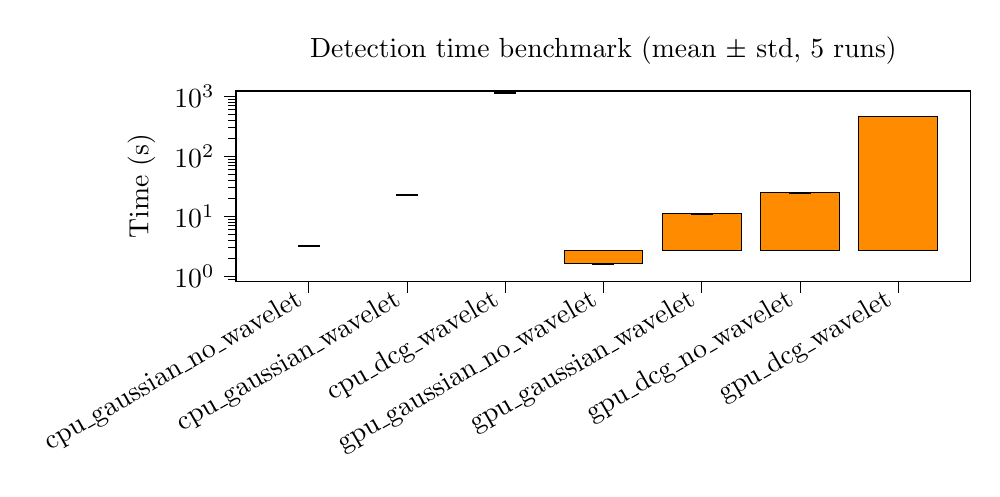
\begin{tikzpicture}

\definecolor{darkgray176}{RGB}{176,176,176}
\definecolor{darkorange}{RGB}{255,140,0}
\definecolor{lightgray204}{RGB}{204,204,204}
\definecolor{steelblue}{RGB}{70,130,180}

\begin{axis}[
height=4cm,
width=0.9\textwidth,
legend cell align={left},
legend style={fill opacity=0.8, draw opacity=1, text opacity=1, draw=lightgray204},
tick align=outside,
tick pos=left,
title={Detection time benchmark (mean ± std, 5 runs)},
x grid style={darkgray176},
xmin=-0.74, xmax=6.74,
xtick style={color=black},
xtick={0,1,2,3,4,5,6},
xticklabel style={rotate=30.0,anchor=east},
xticklabels={
  cpu\_gaussian\_no\_wavelet,
  cpu\_gaussian\_wavelet,
  cpu\_dcg\_wavelet,
  gpu\_gaussian\_no\_wavelet,
  gpu\_gaussian\_wavelet,
  gpu\_dcg\_no\_wavelet,
  gpu\_dcg\_wavelet
},
y grid style={darkgray176},
ylabel={Time (s)},
ymax=1224.04057289162,
ytick style={color=black},
ymode=log
]
\draw[draw=black,fill=darkorange,line width=0.24pt] (axis cs:2.6,0) rectangle (axis cs:3.4,1.61280055962);
\draw[draw=black,fill=darkorange,line width=0.24pt] (axis cs:3.6,0) rectangle (axis cs:4.4,10.98517668238);
\draw[draw=black,fill=darkorange,line width=0.24pt] (axis cs:4.6,0) rectangle (axis cs:5.4,24.66168589718);
\draw[draw=black,fill=darkorange,line width=0.24pt] (axis cs:5.6,0) rectangle (axis cs:6.4,460.99272668412);
\path [draw=black, semithick]
(axis cs:0,3.11705565599688)
--(axis cs:0,3.17154756096312);

\path [draw=black, semithick]
(axis cs:1,22.736708568896)
--(axis cs:1,23.016265406904);

\path [draw=black, semithick]
(axis cs:2,1140.36295115439)
--(axis cs:2,1165.75292656345);

\path [draw=black, semithick]
(axis cs:3,1.59673847648965)
--(axis cs:3,1.62886264275035);

\path [draw=black, semithick]
(axis cs:4,10.9241175710869)
--(axis cs:4,11.0462357936732);

\path [draw=black, semithick]
(axis cs:5,24.5458291466455)
--(axis cs:5,24.7775426477145);

\path [draw=black, semithick]
(axis cs:6,460.326750349203)
--(axis cs:6,461.658703019037);

\addplot [semithick, black, mark=-, mark size=4, mark options={solid}, only marks, forget plot]
table {%
0 3.11705565599688
1 22.736708568896
2 1140.36295115439
3 1.59673847648965
4 10.9241175710869
5 24.5458291466455
6 460.326750349203
};
\addplot [semithick, black, mark=-, mark size=4, mark options={solid}, only marks, forget plot]
table {%
0 3.17154756096312
1 23.016265406904
2 1165.75292656345
3 1.62886264275035
4 11.0462357936732
5 24.7775426477145
6 461.658703019037
};
\end{axis}

\end{tikzpicture}

  
% This file was created with matplot2tikz v0.5.3.
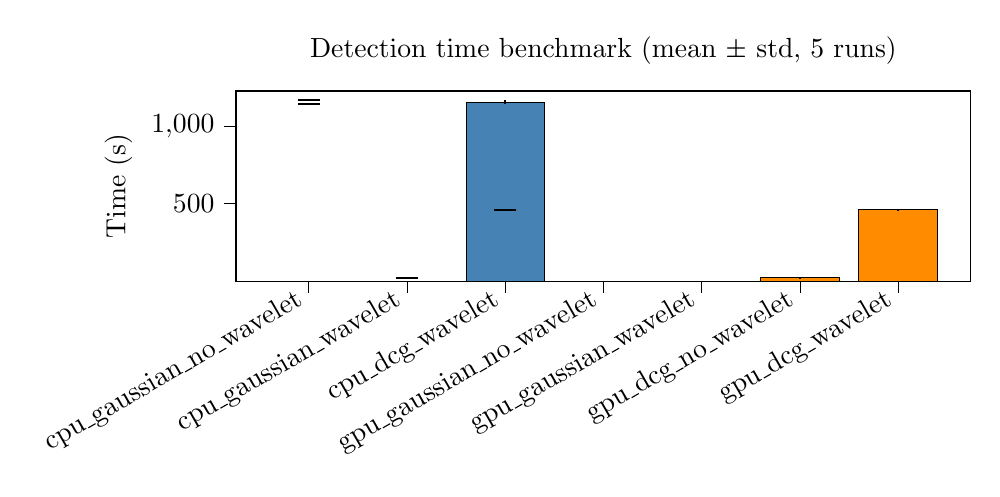
\begin{tikzpicture}

\definecolor{darkgray176}{RGB}{176,176,176}
\definecolor{darkorange}{RGB}{255,140,0}
\definecolor{lightgray204}{RGB}{204,204,204}
\definecolor{steelblue}{RGB}{70,130,180}

\begin{axis}[
height=4cm,
width=0.9\textwidth,
legend cell align={left},
legend style={fill opacity=0.8, draw opacity=1, text opacity=1, draw=lightgray204},
tick align=outside,
tick pos=left,
title={Detection time benchmark (mean ± std, 5 runs)},
x grid style={darkgray176},
xmin=-0.74, xmax=6.74,
xtick style={color=black},
xtick={0,1,2,3,4,5,6},
xticklabel style={rotate=30.0,anchor=east},
xticklabels={
  cpu\_gaussian\_no\_wavelet,
  cpu\_gaussian\_wavelet,
  cpu\_dcg\_wavelet,
  gpu\_gaussian\_no\_wavelet,
  gpu\_gaussian\_wavelet,
  gpu\_dcg\_no\_wavelet,
  gpu\_dcg\_wavelet
},
y grid style={darkgray176},
ylabel={Time (s)},
ymax=1224.04057289162,
ytick style={color=black},
ymin=1,
]
\draw[draw=black,fill=steelblue,line width=0.24pt] (axis cs:1.6,0) rectangle (axis cs:2.4,1153.05793885892);
\draw[draw=black,fill=darkorange,line width=0.24pt] (axis cs:4.6,0) rectangle (axis cs:5.4,24.66168589718);
\draw[draw=black,fill=darkorange,line width=0.24pt] (axis cs:5.6,0) rectangle (axis cs:6.4,460.99272668412);

\path [draw=black, semithick]
(axis cs:2,1140.36295115439)
--(axis cs:2,1165.75292656345);


\path [draw=black, semithick]
(axis cs:5,24.5458291466455)
--(axis cs:5,24.7775426477145);

\path [draw=black, semithick]
(axis cs:6,460.326750349203)
--(axis cs:6,461.658703019037);

\addplot [semithick, black, mark=-, mark size=4, mark options={solid}, only marks, forget plot]
table {%
0 1140.36295115439
1 24.5458291466455
2 460.326750349203
};
\addplot [semithick, black, mark=-, mark size=4, mark options={solid}, only marks, forget plot]
table {%
0 1165.75292656345
1 24.7775426477145
2 461.658703019037
};
\end{axis}

\end{tikzpicture}

  \caption{Comparaison des temps de calculs sur CPU et GPU des cartes de détection de changements sur la Scene 1 avec ($\vdim=12$) ou sans ($\vdim=3$) la décomposition en ondelettes \cite{Mian_wavelet_2019}. Nombre de répétions : 10 (après 5 répétitions de chauffe).}
  \label{fig:benchmark_sar_offline}
\end{figure}



\subsection{Un modèle structuré par le capteur}
\label{subsec:detection-online-riemann}

Le verrou identifié dans l'analyse de complexité qui précède est l'impossibilité de mettre à jour le point fixe sous $\hypothesis_0$. Plutôt que de changer de détecteur, nous proposons de changer la manière de calculer l'estimée: si l'on sait se déplacer le long des géodésiques de la variété sur laquelle vit le paramètre, une seule itération par nouvelle image suffit. Avant d'en venir là, nous profitons de la structure particulière des données pour réduire la dimension du paramètre, ce qui sert à la fois la précision de l'estimation et le coût de chaque itération. Nous présentons d'abord le modèle et le détecteur correspondant, puis la géométrie de la variété, le gradient et l'algorithme récursif, et enfin la borne qui permet de juger l'estimateur obtenu.

\begin{definition}[{Modèle gaussien à échelle et structure de Kronecker}]
\label{def:detection-online-modele}
  On suppose la dispersion structurée en produit de Kronecker $\MScatter = \Kronleft\otimes\Kronright$, avec $\vdim=\dimleft\dimright$, et l'on lève l'ambiguïté d'échelle entre les deux opérandes par une normalisation à déterminant unité. Les observations d'une fenêtre à la date $\itime$ suivent alors
  \begin{equation}
    \x_\iobs^{(\itime)} \sim \cgaussian\left(\vector{0},\,\texture_\iobs\,\Kronleft\otimes\Kronright\right),
    \label{eq:detection-online-modele}
  \end{equation}
  et le paramètre $\param^{(\itime)}=\{\Kronleft^{(\itime)},\Kronright^{(\itime)},\vector{\texture}^{(\itime)}\}$ vit sur la variété produit
  \begin{equation}
    \Manifold = \HPDdet{\dimleft}\times\HPDdet{\dimright}\times\Rpos{\Nobs}.
    \label{eq:detection-online-variete}
  \end{equation}
\end{definition}

Les deux choix de modélisation de la \cref{def:detection-online-modele} ont chacun une raison d'être. La structure de Kronecker n'est pas postulée: elle provient de la transformée en ondelettes de \cite{Mian_wavelet_2019}, qui combine les canaux de polarisation avec une diversité spectro-angulaire. L'un des deux opérandes est alors de taille $3$, le nombre de canaux de polarisation, et l'autre de taille égale au nombre d'intervalles en fréquence et en angle retenus. Comme pour la \cref{prop:detection-fls-kronecker}, la structure est donc héritée du capteur et de la chaîne de traitement, et ses dimensions sont fixées sans paramètre de réglage, contrairement aux structures de rang faible qui demandent d'estimer un rang. La normalisation par le déterminant plutôt que par la trace est quant à elle ce qui rend la métrique de Fisher séparable, comme nous le verrons en \cref{prop:detection-online-metrique}\sideref[-1cm]{prop:context-riemann-detun}{Sous-variété à déterminant unité}.

\begin{proposition}[{glrt structuré}]
\label{prop:detection-online-glrt}
  Le glrt du problème \cref{eq:detection-test-egalite} sous le modèle \cref{eq:detection-online-modele} et pour $\Ntime$ images s'écrit
  \begin{equation}
    \ln\DetectorStat^{(\Ntime)}
    =
    \likelihood_{\hypothesis_1}\left(\{\hat{\param}^{(\itime)}\}_{\itime=1}^{\Ntime}\right)
    - \likelihood_{\hypothesis_0}\left(\hat{\param}^{(0)}\right)
    \detect,
    \label{eq:detection-online-glrt}
  \end{equation}
  où, en notant $q_\iobs^{(\itime)}(\Kronleft,\Kronright) = \x_\iobs^{(\itime)\herm}\inv{(\Kronleft\otimes\Kronright)}\x_\iobs^{(\itime)}$,
  \begin{equation}
    \begin{aligned}
      \likelihood_{\hypothesis_0}\left(\param^{(0)}\right)
      &= -\Ntime\vdim\sum_{\iobs=1}^{\Nobs}\ln\texture_\iobs^{(0)}
         - \sum_{\iobs=1}^{\Nobs}\sum_{\itime=1}^{\Ntime}
           \frac{q_\iobs^{(\itime)}\left(\Kronleft^{(0)},\Kronright^{(0)}\right)}{\texture_\iobs^{(0)}},
      \\
      \likelihood_{\hypothesis_1}\left(\{\param^{(\itime)}\}\right)
      &= -\vdim\sum_{\iobs=1}^{\Nobs}\sum_{\itime=1}^{\Ntime}\ln\texture_\iobs^{(\itime)}
         - \sum_{\iobs=1}^{\Nobs}\sum_{\itime=1}^{\Ntime}
           \frac{q_\iobs^{(\itime)}\left(\Kronleft^{(\itime)},\Kronright^{(\itime)}\right)}{\texture_\iobs^{(\itime)}},
    \end{aligned}
    \label{eq:detection-online-vraisemblances}
  \end{equation}
  les termes en log-déterminant disparaissant du fait de la normalisation à déterminant unité.
\end{proposition}

\begin{proposition}[{Estimateurs du maximum de vraisemblance}]
\label{prop:detection-online-mle}
  En notant $\obsmat_{\iobs\itime}\in\C^{\dimright\times\dimleft}$ la matrice telle que $\vecop(\obsmat_{\iobs\itime})=\x_\iobs^{(\itime)}$, les estimateurs sous $\hypothesis_0$ sont solutions du système de points fixes
  \begin{equation}
    \left\{
    \begin{aligned}
      \widehat{\Kronleft}^{(0)} &= \frac{1}{\Ntime\Nobs\dimright}
        \sum_{\itime=1}^{\Ntime}\sum_{\iobs=1}^{\Nobs}
        \frac{\obsmat_{\iobs\itime}^\T\,\conj{\left(\widehat{\Kronright}^{(0)}\right)^{-1}}\,\conj{\obsmat_{\iobs\itime}}}{\hat{\texture}_\iobs^{(0)}},
      \\
      \widehat{\Kronright}^{(0)} &= \frac{1}{\Ntime\Nobs\dimleft}
        \sum_{\itime=1}^{\Ntime}\sum_{\iobs=1}^{\Nobs}
        \frac{\obsmat_{\iobs\itime}\,\conj{\left(\widehat{\Kronleft}^{(0)}\right)^{-1}}\,\obsmat_{\iobs\itime}^\herm}{\hat{\texture}_\iobs^{(0)}},
      \\
      \hat{\texture}_\iobs^{(0)} &= \frac{1}{\Ntime\vdim}\sum_{\itime=1}^{\Ntime}
        q_\iobs^{(\itime)}\left(\widehat{\Kronleft}^{(0)},\widehat{\Kronright}^{(0)}\right),
    \end{aligned}
    \right.
    \label{eq:detection-online-mle}
  \end{equation}
  ceux sous $\hypothesis_1$ s'en déduisant en supprimant la sommation sur $\itime$ et les facteurs $\Ntime$ correspondants.
\end{proposition}

On remarquera que les estimateurs sous $\hypothesis_1$ coïncident avec l'estimateur de Tyler à structure de Kronecker de \sidecite{sun2016robust}, à la conjugaison près puisque nous traitons des données complexes. C'est le même objet que celui de la \cref{subsec:detection-fls-estimation}, sans la contrainte de Toeplitz. Ceux sous $\hypothesis_0$ en diffèrent par la sommation sur $\itime$, qui traduit le partage du paramètre entre les dates. C'est cette sommation, prise à l'intérieur d'un point fixe, qui interdit la mise à jour récursive:

\begin{property}[{Non-récursivité du point fixe}]
\label{prop:detection-online-nonrecursif}
  À l'arrivée d'une nouvelle image, l'estimée sous $\hypothesis_0$ ne se met pas à jour comme une moyenne des estimées passées:
  \begin{equation}
    \widehat{\Kronleft}^{(0)}\left(\Xset_{1:\Ntime+1}\right)
    \neq
    \frac{\Ntime}{\Ntime+1}\widehat{\Kronleft}^{(0)}\left(\Xset_{1:\Ntime}\right)
    + \frac{1}{\Ntime+1}\widehat{\Kronleft}^{(0)}\left(\Xset_{\Ntime+1}\right),
    \label{eq:detection-online-nonrecursif}
  \end{equation}
  et il en va de même pour $\Kronright$ et pour les textures.
\end{property}

La structure ne lève donc pas le verrou mis en évidence pour le GLRT non-gaussien \eqref{eq:glrt_nongaussian_cd}: elle réduit le coût de chaque itération du point fixe, mais il faut toujours reprendre l'ensemble des $\Ntime+1$ dates à l'arrivée d'une nouvelle image.

\subsection{La géométrie de l'information du modèle}

Pour construire une mise à jour récursive\sideref{prop:context-geometry-fisherccg}{Métrique de Fisher du modèle gaussien composé}, nous avons besoin d'une géométrie sur $\Manifold$. Le choix naturel est celle induite par la métrique de Fisher du modèle, dont nous avons vu qu'elle se décompose sur une variété produit dans le cas d'une gaussienne composée sans structure. La proposition suivante étend ce résultat à la structure de Kronecker.

\begin{proposition}[{Métrique de Fisher sur $\Manifold$}]
\label{prop:detection-online-metrique}
  Pour $\param\in\Manifold$ et $\tvec=(\tvec_{\Kronleft},\tvec_{\Kronright},\tvec_{\vector{\texture}})$, $\tvecbis=(\tvecbis_{\Kronleft},\tvecbis_{\Kronright},\tvecbis_{\vector{\texture}})$ dans $\Tangent{\param}{\Manifold}$, la métrique de Fisher induite par le modèle \cref{eq:detection-online-modele} s'écrit
  \begin{equation}
    \begin{aligned}
      \metric{\tvec}{\tvecbis}{\param}
      ={}&
      \frac{\dimright}{\vdim}\trace{\inv{\Kronleft}\tvec_{\Kronleft}\inv{\Kronleft}\tvecbis_{\Kronleft}}
      + \frac{\dimleft}{\vdim}\trace{\inv{\Kronright}\tvec_{\Kronright}\inv{\Kronright}\tvecbis_{\Kronright}}
      \\
      &+ \frac{1}{\Nobs}\left(\tvec_{\vector{\texture}}\had\hadinv{\vector{\texture}}\right)^\T
        \left(\tvecbis_{\vector{\texture}}\had\hadinv{\vector{\texture}}\right),
    \end{aligned}
    \label{eq:detection-online-metrique}
  \end{equation}
  où $\had$ désigne le produit de Hadamard. Les espaces tangents aux deux facteurs matriciels sont
  \begin{equation}
    \Tangent{\Kronleft}{\HPDdet{\dimleft}}
    = \left\{\tvec_{\Kronleft}\in\Herm{\dimleft}\ :\ \trace{\inv{\Kronleft}\tvec_{\Kronleft}}=0\right\},
    \label{eq:detection-online-tangent}
  \end{equation}
  et de même pour $\Kronright$.
\end{proposition}

La métrique \cref{eq:detection-online-metrique} est la somme de deux métriques affines invariantes, pondérées par $\dimright/\vdim$ et $\dimleft/\vdim$, et d'un terme sur les textures. Il n'y a aucun terme croisé entre les trois facteurs, ce qui n'aurait pas été le cas avec une normalisation par la trace. La géométrie de $\Manifold$ s'obtient alors en combinant celle de chaque facteur:

\begin{property}[{Exponentielle et distance}]
\label{prop:detection-online-expdist}
  La métrique \cref{eq:detection-online-metrique} étant séparable, l'exponentielle riemannienne et la distance géodésique se calculent composante par composante:
  \begin{equation}
    \begin{aligned}
      \exp_{\param}(\tvec)
      ={}&
      \Big(
        \Kronleft\,\expm\left(\inv{\Kronleft}\tvec_{\Kronleft}\right),\
        \Kronright\,\expm\left(\inv{\Kronright}\tvec_{\Kronright}\right),
      \\
      &\phantom{\Big(}\vector{\texture}\had\exp\big(\hadinv{\vector{\texture}}\had\tvec_{\vector{\texture}}\big)
      \Big),
    \end{aligned}
    \label{eq:detection-online-exp}
  \end{equation}
  \begin{equation}
    \begin{aligned}
      \geodist^2_{\Manifold}(\param_0,\param_1)
      ={}&
      \frac{\dimright}{\vdim}\geodist^2_{\HPD{\dimleft}}(\Kronleft_0,\Kronleft_1)
      + \frac{\dimleft}{\vdim}\geodist^2_{\HPD{\dimright}}(\Kronright_0,\Kronright_1)
      \\
      &+ \frac{1}{\Nobs}\norm{\ln\left(\hadinv{\vector{\texture}_0}\had\vector{\texture}_1\right)}_2^2.
    \end{aligned}
    \label{eq:detection-online-dist}
  \end{equation}
\end{property}

\subsection{Pourquoi un gradient naturel stochastique}

Disposant de la géométrie de $\Manifold$, il reste à choisir comment mettre à jour l'estimée sous $\hypothesis_0$ à l'arrivée d'une nouvelle fenêtre $\Xset_{\Ntime+1}$. L'idée est de ne faire qu'un pas de gradient riemannien\sideref[-0.8cm]{def:context-riemann-gradient}{Gradient riemannien}, calculé sur la seule vraisemblance de la nouvelle fenêtre, au lieu de résoudre à nouveau le point fixe sur toutes les dates. Rappelons que l'algorithme de point fixe d'un M-estimateur est lui-même une descente de gradient riemannienne à pas constant\sideref[0.4cm]{prop:context-riemann-pointfixe}{Le point fixe comme descente de gradient}: le schéma proposé n'en est donc qu'une version stochastique, où chaque date apporte un pas dont la taille décroît en $1/\Ntime$.

\begin{proposition}[{Gradient riemannien}]
\label{prop:detection-online-gradient}
  Le gradient riemannien de la log-vraisemblance de la seule nouvelle fenêtre $\likelihood^{(\Ntime+1)}$, au sens de la métrique \cref{eq:detection-online-metrique}, vaut
  \begin{equation}
    \Rgrad\likelihood^{(\Ntime+1)}(\param)
    =
    \left(\mat{G}_{\Kronleft},\,\mat{G}_{\Kronright},\,\vector{g}_{\vector{\texture}}\right),
    \qquad
    \left\{
    \begin{aligned}
      \mat{G}_{\Kronleft} &= \frac{\vdim}{\dimright}\sum_{\iobs=1}^{\Nobs}\frac{\projman_{\Kronleft}\left(\obsmat_\iobs^\T\Kronright^{-\T}\conj{\obsmat_\iobs}\right)}{\texture_\iobs},\\
      \mat{G}_{\Kronright} &= \frac{\vdim}{\dimleft}\sum_{\iobs=1}^{\Nobs}\frac{\projman_{\Kronright}\left(\obsmat_\iobs\Kronleft^{-\T}\obsmat_\iobs^\herm\right)}{\texture_\iobs},\\
      \vector{g}_{\vector{\texture}} &= \Nobs\left(\vector{q}^{(\Ntime+1)}-\vdim\,\vector{\texture}\right),
    \end{aligned}
    \right.
    \label{eq:detection-online-gradient}
  \end{equation}
  où $\vector{q}^{(\Ntime+1)}$ rassemble les formes quadratiques $q_\iobs^{(\Ntime+1)}(\Kronleft,\Kronright)$ et où la projection sur l'espace tangent \cref{eq:detection-online-tangent} s'écrit
  \begin{equation}
    \projman_{\Kronleft}\left(\tvec_{\Kronleft}\right)
    =
    \tvec_{\Kronleft} - \frac{\trace{\inv{\Kronleft}\tvec_{\Kronleft}}}{\dimleft}\,\Kronleft.
    \label{eq:detection-online-projection}
  \end{equation}
\end{proposition}

\begin{definition}[{Montée de gradient naturel stochastique}]
\label{def:detection-online-sgd}
  L'estimée sous $\hypothesis_0$ est mise à jour, à l'arrivée de la fenêtre $\Xset_{\Ntime+1}$, par une unique itération
  \begin{equation}
    \hat{\param}^{(0)}_{\Xset_{1:\Ntime+1}}
    =
    \exp_{\hat{\param}^{(0)}_{\Xset_{1:\Ntime}}}
    \left(
      \frac{\alpha_0}{\Ntime}\,\Rgrad\likelihood^{(\Ntime+1)}\left(\hat{\param}^{(0)}_{\Xset_{1:\Ntime}}\right)
    \right),
    \qquad
    \alpha_0=\frac{1}{\vdim\Nobs}.
    \label{eq:detection-online-sgd}
  \end{equation}
\end{definition}

Le choix $\alpha_0=1/(\vdim\Nobs)$ se lit directement sur la composante des textures. Au premier ordre, la mise à jour \cref{eq:detection-online-sgd} donne en effet
\begin{equation*}
  \hat{\texture}_\iobs^{(0)} \leftarrow \hat{\texture}_\iobs^{(0)} + \frac{1}{\Ntime}\left(\frac{q_\iobs^{(\Ntime+1)}}{\vdim}-\hat{\texture}_\iobs^{(0)}\right),
\end{equation*}
c'est-à-dire une moyenne courante des estimées de texture date par date, ce qui est exactement la forme de $\hat{\texture}_\iobs^{(0)}$ dans \cref{eq:detection-online-mle}. Il en va de même pour $\Kronleft$ et $\Kronright$, dont le pas est la projection sur l'espace tangent de l'écart entre le terme du point fixe calculé sur la nouvelle fenêtre et l'estimée courante. La procédure complète est résumée dans l'\cref{alg:detection-online}.

\begin{algorithm}[htbp]
\caption{Détection de changements en ligne}
\label{alg:detection-online}
\begin{algorithmic}[1]
  \Require $\hat{\param}^{(0)}$ initialisée sur la première fenêtre, statistique courante $\ln\DetectorStat^{(\Ntime)}$
  \For{chaque nouvelle image $\Ntime+1$}
    \State calculer $\Rgrad\likelihood^{(\Ntime+1)}(\hat{\param}^{(0)})$ par \cref{eq:detection-online-gradient}
    \State $\hat{\param}^{(0)} \gets \exp_{\hat{\param}^{(0)}}\left(\dfrac{\alpha_0}{\Ntime}\Rgrad\likelihood^{(\Ntime+1)}(\hat{\param}^{(0)})\right)$ par \cref{eq:detection-online-exp}
    \State estimer $\hat{\param}^{(\Ntime+1)}$ sous $\hypothesis_1$ sur la seule fenêtre courante par \cref{eq:detection-online-mle}
    \State mettre à jour $\ln\DetectorStat^{(\Ntime+1)}$ par \cref{eq:detection-online-glrt}
  \EndFor
\end{algorithmic}
\end{algorithm}

Le fait d'employer le gradient \emph{naturel}, c'est-à-dire le gradient associé à la métrique de Fisher, plutôt qu'une descente riemannienne quelconque, a deux conséquences pratiques. D'une part, le pas optimal s'obtient analytiquement et ne dépend que des dimensions intrinsèques $(\dimleft,\dimright,\Nobs)$ du problème: aucune recherche linéaire n'est nécessaire, et le coût par image est réellement constant. D'autre part, la descente stochastique associée est statistiquement efficace \cite{Zhou_2019}: l'estimée récursive tend vers l'estimateur du maximum de vraisemblance sous $\hypothesis_0$ lorsque $\Ntime\to\infty$, de sorte que le glrt en ligne est asymptotiquement équivalent au glrt hors ligne et que l'on peut remplacer l'un par l'autre sans changer la règle de décision.

Plus précisément, chaque nouvelle image demande l'inversion de $\Kronleft$ et $\Kronright$, le calcul des $\Nobs$ produits $\obsmat_\iobs^\T\Kronright^{-\T}\conj{\obsmat_\iobs}$ et $\obsmat_\iobs\Kronleft^{-\T}\obsmat_\iobs^\herm$, puis deux exponentielles de matrices de tailles $\dimleft$ et $\dimright$, soit un coût en $\bigO(\Nobs\vdim(\dimleft+\dimright)+\dimleft^3+\dimright^3)$ qui ne dépend pas de $\Ntime$\footnote{Pour évaluer $\likelihood_{\hypothesis_0}$ dans \cref{eq:detection-online-glrt} sans revenir aux données passées, il suffit de conserver pour chaque pixel de la fenêtre la somme $\sum_{\itime}\x_\iobs^{(\itime)}\x_\iobs^{(\itime)\herm}$, puisque $\sum_\itime q_\iobs^{(\itime)}$ en est une fonction linéaire.}. On le comparera au $\bigO(\Niter\Ntime\vdim^3)$ établi plus haut pour la version hors ligne.
% TODO a verifier: le cout par image ci-dessus est derive a la main (produits
% de taille (a x b)(b x b)(b x a)), il n'est pas donne dans l'article.

\subsection{Une borne pour juger l'estimateur}

Pour juger de la qualité de l'estimée récursive, il reste à disposer d'une référence. La borne de Cramér-Rao intrinsèque\sideref{sec:context-geometry-icrb}{Borne de Cramér-Rao intrinsèque} s'applique ici telle quelle: la contrainte de déterminant unité et la structure de Kronecker sont portées par la variété $\Manifold$ elle-même, et il suffit de travailler dans son espace tangent. La distance \cref{eq:detection-online-dist} étant celle de la métrique de Fisher, la borne prend une forme particulièrement simple.

\begin{proposition}[{Borne de Cramér-Rao intrinsèque}]
\label{prop:detection-online-icrb}
  Pour un estimateur non biaisé $\hat{\param}^{(\Ntime)}$ construit sur $\Ntime$ dates, l'erreur mesurée par la distance \cref{eq:detection-online-dist} est minorée par
  \begin{equation}
    \E\left\{\geodist^2_{\Manifold}\left(\param^{(\Ntime)},\hat{\param}^{(\Ntime)}\right)\right\}
    \geq
    \frac{\left(\dimleft^2-1\right)+\left(\dimright^2-1\right)+\Nobs}{\Ntime\,\vdim\,\Nobs},
    \label{eq:detection-online-icrb}
  \end{equation}
  et, la métrique étant séparable, composante par composante:
  \begin{equation}
    \E\left\{\geodist^2_{\HPD{\dimleft}}\right\} \geq \frac{\dimleft^2-1}{\dimright\,\Ntime\,\Nobs},
    \qquad
    \E\left\{\geodist^2_{\HPD{\dimright}}\right\} \geq \frac{\dimright^2-1}{\dimleft\,\Ntime\,\Nobs},
    \qquad
    \E\left\{\geodist^2_{\Rpos{\Nobs}}\right\} \geq \frac{\Nobs}{\Ntime\,\vdim}.
    \label{eq:detection-online-icrb-composantes}
  \end{equation}
\end{proposition}

La lecture de la borne est directe. Le numérateur de \cref{eq:detection-online-icrb} compte les paramètres à estimer, soit $\dimleft^2-1$ et $\dimright^2-1$ pour les deux facteurs une fois la contrainte de déterminant prise en compte, plus les $\Nobs$ textures, et le dénominateur compte les données réelles disponibles. On retrouve donc le comptage de la \cref{prop:detection-fls-comptage}, vu cette fois du côté de l'erreur d'estimation. C'est aussi ce qui permet de mesurer ce que la structure apporte: à $\vdim=12$ et $\Nobs=13$, la borne de la dispersion structurée est plus faible d'un facteur $156/36\simeq4{,}3$ que celle d'une dispersion libre dans $\HPDdet{\vdim}$.

\subsection{Ce que la mise en ligne coûte et rapporte}

Les simulations ci-dessous reprennent celles de \cite{SP24} en les complétant. Les données sont K-distribuées ($\nu=1$) ou gaussiennes, avec $\dimleft=3$, $\dimright=4$, $\Nobs=13$ et des facteurs de Toeplitz\footnote{Ce sont les paramètres des légendes de figures et du code diffusé avec \cite{SP24}; le texte de l'article annonce $\dimleft=4$, $\dimright=3$, $\Nobs=8$ et des facteurs aléatoires. Nous retenons les premiers pour que les figures restent comparables à celles de l'article.}. Elles conduisent aux constats suivants:
\begin{itemize}
  \item l'estimateur hors ligne suit les bornes \cref{eq:detection-online-icrb-composantes} sur toute la plage de $\Ntime$, et l'estimateur récursif, qui n'effectue qu'un pas par nouvelle image, les rejoint: à $\Ntime=10^3$, les trois composantes sont à la borne (\cref{fig:detection-online-mse-icrb});
  \item à nombre de dates fixé, chaque estimateur atteint sa propre borne, et l'écart mesuré entre structure de Kronecker et dispersion libre est de $4{,}5$ à $\Nobs=13$, pour $4{,}3$ prédit par le rapport des dimensions. Le gain va de $5{,}9$ à $\Nobs=4$ à $2{,}3$ à $\Nobs=70$: la structure apporte d'autant plus que la fenêtre est petite (\cref{fig:detection-online-structure});
  \item en détection, en fouillis K-distribué, le glrt structuré en ligne suit de près sa version hors ligne dès les premières dates, avec un creux transitoire vers $\Ntime=7$ dû au démarrage sur l'estimée de la première date (\cref{fig:detection-online-puissance});
  \item en fouillis gaussien, les détecteurs en ligne rejoignent aussi leur contrepartie hors ligne, mais bien plus tard: à $\Ntime=49$, la puissance est de $0{,}981$ pour le glrt structuré en ligne contre $0{,}999$ hors ligne (\cref{fig:detection-online-puissance-gaussien}). L'article signalait déjà cette convergence plus lente en milieu quasi gaussien, que nous présentons ici comme une observation.
\end{itemize}

% ============================== FIGURE 9/9 =========================================
% Elle porte la these de la section. Run pleine echelle (1000 tirages, T
% jusqu'a 1000), qanat: sar_mc_kron_mse.
%
% ATTENTION aux parametres, ils ne sont PAS ceux annonces dans le corps de
% \fullcite{SP24}: le texte du paragraphe 5.1 annonce $\dimleft=4$,
% $\dimright=3$, $\Nobs=8$ et des facteurs aleatoires de conditionnement 10,
% alors que les legendes des figures publiees et le code diffuse utilisent
% $\dimleft=3$, $\dimright=4$, $\Nobs=13$ et des facteurs Toeplitz. Ce sont ces
% derniers qui sont implementes ici, pour que la figure du memoire soit
% comparable a celles de l'article. A signaler en note de bas de page.
%
% Deux erratum de l'article a redresser silencieusement dans le texte:
%  - la proposition 2 intervertit les poids $a/p$ et $b/p$ de la metrique; la
%    derivation donne $b/p$ devant le terme en $\Kronleft$, et l'eq. (25) est
%    coherente avec ce choix, pas avec la proposition;
%  - la troisieme ligne de l'eq. (25) oublie un facteur $\Nobs$ sur l'icrb de
%    la texture: le decompte de dimensions donne $\Nobs/(\Ntime\vdim)$.
% Le code de \cref{eq:detection-online-icrb-composantes} implemente les formules
% corrigees; verifier que les equations du memoire les reprennent.
% ====================================================================================
\begin{figure}[htbp]
  \centering
  % This file was created with matplot2tikz v0.5.3.
\begin{tikzpicture}

\definecolor{cornflowerblue92168211}{RGB}{92,168,211}
\definecolor{darkgray176}{RGB}{176,176,176}
\definecolor{indianred224107107}{RGB}{224,107,107}
\definecolor{slategray107114128}{RGB}{107,114,128}

\begin{groupplot}[group style={group size=1 by 3, vertical sep=1.5cm, horizontal sep=1.4cm}]
\nextgroupplot[
height=5cm,
label style={font=\footnotesize},
legend cell align={left},
legend style={
  fill opacity=0.8,
  draw opacity=1,
  text opacity=1,
  at={(1.02,1)},
  anchor=north west,
  draw=none
},
legend style={draw=none, fill=white, fill opacity=0.9, text opacity=1, font=\footnotesize},
log basis x={10},
log basis y={10},
scaled x ticks=manual:{}{\pgfmathparse{#1}},
tick align=outside,
tick label style={font=\scriptsize},
tick pos=left,
title style={font=\footnotesize, yshift=-2pt},
width=\textwidth,
x grid style={darkgray176},
xmin=1.46582287710854, xmax=1364.42133032142,
xmode=log,
xtick style={color=black},
xticklabels={},
y grid style={darkgray176},
ylabel={\(\displaystyle \delta^2(\widehat{A}, A)\)},
ymin=0.000105367752356983, ymax=0.43555611672202,
ymode=log,
ytick style={color=black}
]
\addplot [semithick, cornflowerblue92168211, mark=*, mark size=1.5, mark options={solid}]
table {%
2 0.0895362072745407
3 0.0585250003243519
6 0.0283818747888864
10 0.0170455421867386
19 0.00901766335281634
33 0.00505913064871527
59 0.00286068707341474
104 0.00159307677379477
183 0.000909619674187899
323 0.000513237021196533
568 0.000289219537766023
1000 0.000165293174984273
};
\addlegendentry{hors ligne}
\addplot [semithick, indianred224107107, dashed, mark=square*, mark size=1.5, mark options={solid}]
table {%
2 0.298308198788178
3 0.184877961657095
6 0.0759566080980669
10 0.0379719601807544
19 0.0156387605264035
33 0.0074149722444299
59 0.0035322310049275
104 0.00177689296271305
183 0.000942238911006688
323 0.000506127381157759
568 0.000276611778717077
1000 0.000155866462051673
};
\addlegendentry{en ligne}
\addplot [semithick, slategray107114128, dotted]
table {%
2 0.0769230769230769
3 0.0512820512820513
6 0.0256410256410256
10 0.0153846153846154
19 0.00809716599190283
33 0.00466200466200466
59 0.00260756192959583
104 0.0014792899408284
183 0.000840689365279529
323 0.000476303881876637
568 0.000270855904658722
1000 0.000153846153846154
};
\addlegendentry{ICRB}

\nextgroupplot[
height=5cm,
label style={font=\footnotesize},
legend style={draw=none, fill=white, fill opacity=0.9, text opacity=1, font=\footnotesize},
log basis x={10},
log basis y={10},
scaled x ticks=manual:{}{\pgfmathparse{#1}},
tick align=outside,
tick label style={font=\scriptsize},
tick pos=left,
title style={font=\footnotesize, yshift=-2pt},
width=\textwidth,
x grid style={darkgray176},
xmin=1.46582287710854, xmax=1364.42133032142,
xmode=log,
xtick style={color=black},
xticklabels={},
y grid style={darkgray176},
ylabel={\(\displaystyle \delta^2(\widehat{B}, B)\)},
ymin=0.000265041072798692, ymax=0.957215117111117,
ymode=log,
ytick style={color=black}
]
\addplot [semithick, cornflowerblue92168211, mark=*, mark size=1.5, mark options={solid}]
table {%
2 0.223442198207922
3 0.145881632952956
6 0.0722976463209531
10 0.0427686063373079
19 0.0222007256115457
33 0.0127560528414048
59 0.00702757966477109
104 0.00402917584783066
183 0.00229644388946967
323 0.00131546089002939
568 0.000738738696475272
1000 0.000417911639911611
};
\addplot [semithick, indianred224107107, dashed, mark=square*, mark size=1.5, mark options={solid}]
table {%
2 0.659623435999464
3 0.423009213413227
6 0.18068115775155
10 0.092296437960212
19 0.0388002111167975
33 0.0185913474984134
59 0.0088901378677693
104 0.00454924646454687
183 0.00241223010235015
323 0.0013014865625888
568 0.000708554832091816
1000 0.000396190985679097
};
\addplot [semithick, slategray107114128, dotted]
table {%
2 0.192307692307692
3 0.128205128205128
6 0.0641025641025641
10 0.0384615384615385
19 0.0202429149797571
33 0.0116550116550117
59 0.00651890482398957
104 0.00369822485207101
183 0.00210172341319882
323 0.00119075970469159
568 0.000677139761646804
1000 0.000384615384615385
};

\nextgroupplot[
height=5cm,
label style={font=\footnotesize},
legend style={draw=none, fill=white, fill opacity=0.9, text opacity=1, font=\footnotesize},
log basis x={10},
log basis y={10},
tick align=outside,
tick label style={font=\scriptsize},
tick pos=left,
title style={font=\footnotesize, yshift=-2pt},
width=\textwidth,
x grid style={darkgray176},
xlabel={\(\displaystyle T\)},
xmin=1.46582287710854, xmax=1364.42133032142,
xmode=log,
xtick style={color=black},
y grid style={darkgray176},
ylabel={\(\displaystyle \delta^2(\widehat{\tau}, \tau)\)},
ymin=0.000679756960637363, ymax=18.9518906932137,
ymode=log,
ytick style={color=black}
]
\addplot [semithick, cornflowerblue92168211, mark=*, mark size=1.5, mark options={solid}]
table {%
2 0.62939263893048
3 0.399075723270863
6 0.189948284844598
10 0.110562649303202
19 0.0572000061557415
33 0.0329593198533713
59 0.0185635734230305
104 0.0105403685209879
183 0.00601958547457693
323 0.00336165607452135
568 0.00191544104491014
1000 0.00108246210984381
};
\addplot [semithick, indianred224107107, dashed, mark=square*, mark size=1.5, mark options={solid}]
table {%
2 11.9012753414614
3 6.61131749236055
6 2.40270177384308
10 1.11187634892263
19 0.407163190079277
33 0.169399542992606
59 0.0664542272658375
104 0.0274448661447658
183 0.0118502375814403
323 0.00532110882038997
568 0.00255664425714164
1000 0.00129075124845587
};
\addplot [semithick, slategray107114128, dotted]
table {%
2 0.541666666666667
3 0.361111111111111
6 0.180555555555556
10 0.108333333333333
19 0.0570175438596491
33 0.0328282828282828
59 0.018361581920904
104 0.0104166666666667
183 0.00591985428051002
323 0.00335397316821465
568 0.00190727699530516
1000 0.00108333333333333
};
\end{groupplot}

\end{tikzpicture}

  \provMseIcrbQR[1cm]
  \caption{Erreur quadratique riemannienne sur chaque composante de
  $\param=(\Kronleft,\Kronright,\vector{\texture})$ en fonction du nombre de
  dates $\Ntime$, pour des donnees K-distribuees ($\nu=1$), $\dimleft=3$,
  $\dimright=4$, $\Nobs=13$, moyennee sur $10^3$ tirages. L'estimateur hors
  ligne suit les bornes intrinseques de Cramer-Rao
  \eqref{eq:detection-online-icrb-composantes} (pointilles) sur toute la plage;
  l'estimateur recursif \eqref{eq:detection-online-sgd}, qui n'effectue qu'un
  seul pas de gradient par nouvelle image, les rejoint. À $\Ntime=10^3$ les
  trois composantes sont à la borne: la mise en ligne ne se paie pas en
  precision. \provMseIcrb}
  \label{fig:detection-online-mse-icrb}
\end{figure}

% ============================ FIGURE SUPPLEMENTAIRE ================================
% Ajoutee au plan initial (validee le 2026-08-25). Elle referme le fil du
% chapitre: le \cref{sec:detection-fls} contraint le MODELE pour baisser le
% $\Nobs$ necessaire, cette section contraint le CALCUL --- et cette figure
% mesure le premier levier sur le modele de la detection de changements, donc
% avec les memes outils que le second. Sans elle, l'annonce de plan faite en
% \cref{sec:detection-cadre} n'est jamais verifiee.
%
% Chiffres a citer dans le texte: le rapport des dimensions vaut
% $((\dimleft^2-1)+(\dimright^2-1)+\Nobs)/((\vdim^2-1)+\Nobs) = 36/156$ a
% $\Nobs=13$, soit un facteur 4,3 sur la borne --- et l'experience donne 4,5.
% Le gain mesure va de 5,9 a $\Nobs=4$ jusqu'a 2,3 a $\Nobs=70$: la structure
% achete d'autant plus que la fenetre est petite.
% ====================================================================================
\begin{figure}[htbp]
  \centering
  % This file was created with matplot2tikz v0.5.3.
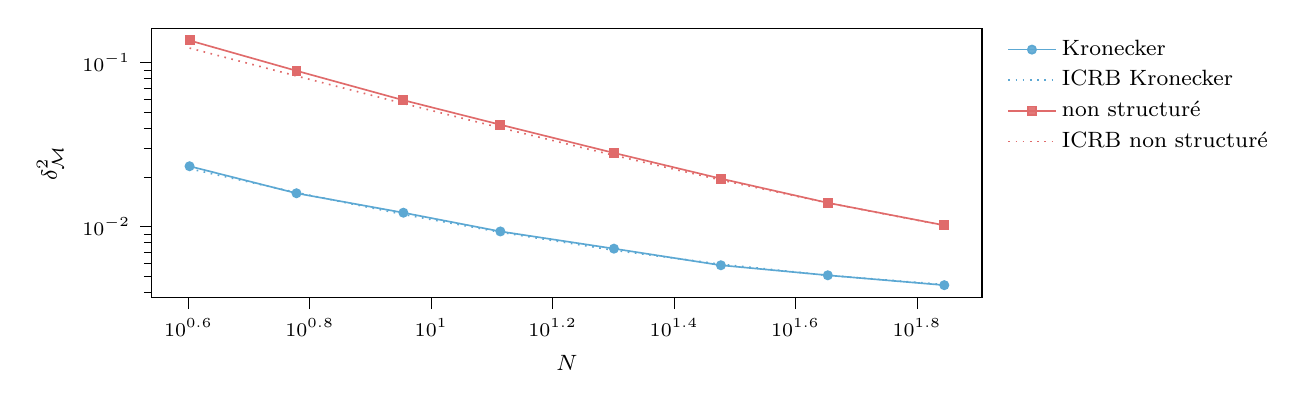
\begin{tikzpicture}

\definecolor{cornflowerblue92168211}{RGB}{92,168,211}
\definecolor{darkgray176}{RGB}{176,176,176}
\definecolor{indianred224107107}{RGB}{224,107,107}

\begin{axis}[
height=5cm,
label style={font=\footnotesize},
legend cell align={left},
legend style={
  fill opacity=0.8,
  draw opacity=1,
  text opacity=1,
  at={(1.02,1)},
  anchor=north west,
  draw=none
},
legend style={draw=none, fill=white, fill opacity=0.9, text opacity=1, font=\footnotesize},
log basis x={10},
log basis y={10},
tick align=outside,
tick label style={font=\scriptsize},
tick pos=left,
title style={font=\footnotesize, yshift=-2pt},
width=\textwidth,
x grid style={darkgray176},
xlabel={\(\displaystyle N\)},
xmin=3.46663477207328, xmax=80.7699738823485,
xmode=log,
xtick style={color=black},
y grid style={darkgray176},
ylabel={\(\displaystyle \delta^2_{\mathcal{M}}\)},
ymin=0.00369701384829338, ymax=0.161889573881461,
ymode=log,
ytick style={color=black}
]
\addplot [semithick, cornflowerblue92168211, mark=*, mark size=1.5, mark options={solid}]
table {%
4 0.0233147832541332
6 0.0159525050224172
9 0.0121408491355551
13 0.00933346500175258
20 0.00732975415768509
30 0.0058054613688464
45 0.00504288206267022
70 0.00438994121535721
};
\addlegendentry{Kronecker}
\addplot [semithick, cornflowerblue92168211, dotted]
table {%
4 0.0225
6 0.0161111111111111
9 0.0118518518518519
13 0.00923076923076923
20 0.00716666666666667
30 0.00588888888888889
45 0.00503703703703704
70 0.00442857142857143
};
\addlegendentry{ICRB Kronecker}
\addplot [semithick, indianred224107107, mark=square*, mark size=1.5, mark options={solid}]
table {%
4 0.136336221186819
6 0.0890602056750955
9 0.0589364835787556
13 0.041775386637242
20 0.0281039615846208
30 0.0195927266801986
45 0.0139482758019912
70 0.0101782921379158
};
\addlegendentry{non structuré}
\addplot [semithick, indianred224107107, dotted]
table {%
4 0.1225
6 0.0827777777777778
9 0.0562962962962963
13 0.04
20 0.0271666666666667
30 0.0192222222222222
45 0.0139259259259259
70 0.0101428571428571
};
\addlegendentry{ICRB non structuré}
\end{axis}

\end{tikzpicture}

  \provStructureVsNQR[.5cm]
  \caption{Ce que la structure achete: erreur totale $\delta^2_\Manifold$ en
  fonction de la taille $\Nobs$ de la fenetre, à nombre de dates fixe
  ($\Ntime=25$), pour la dispersion contrainte en produit de Kronecker et pour
  la dispersion libre dans $\HPDdet{\vdim}$. Meme geometrie, meme gradient,
  meme recherche lineaire des deux cotes: seul l'espace de parametres change.
  Chaque estimateur atteint sa propre borne (pointilles), et l'ecart entre les
  deux bornes est un rapport de dimensions, large sur les petites fenetres et
  qui se referme quand $\Nobs$ croit. \provStructureVsN}
  \label{fig:detection-online-structure}
\end{figure}

% ============================ FIGURE SUPPLEMENTAIRE ================================
% Remplace les trois planches de courbes roc de \fullcite{SP24} (figures 4 a 6),
% jugees redondantes: douze courbes pour une conclusion qui tient en une phrase.
% La puissance a $\pfa$ fixee en fonction de $\Ntime$ dit la meme chose sur un
% seul axe, et c'est le seul axe dont la section a besoin: a quelle vitesse le
% detecteur en ligne rattrape-t-il le hors ligne.
%
% Le pendant gaussien est la figure suivante. C'est la comparaison des deux qui
% porte le propos: l'heterogeneite aide le schema stochastique.
%
% TODO a verifier avant redaction: a ce reglage ($\Nobs=13$, $\vdim=12$), les
% deux detecteurs NON structures n'ont quasiment aucune puissance (0,03), alors
% que les roc de l'article a $\Ntime=50$ les montrent utilisables. Vient
% probablement de l'amplitude du changement ou du $\pfa$ retenu; a regarder
% avant d'en tirer un argument, sinon la figure prouve trop.
%
% A commenter aussi: le creux du detecteur structure en ligne vers $\Ntime=7$
% (0,96 a $\Ntime=2$, 0,71 a $\Ntime=7$, 1,00 a $\Ntime=49$). Ce n'est pas du
% bruit: le demarrage se fait sur l'estimee mm de la premiere date, que les
% premiers pas de gradient degradent avant que le moyennage en $\alpha_0/\Ntime$
% ne reprenne la main.
% ====================================================================================
\begin{figure}[htbp]
  \centering
  % This file was created with matplot2tikz v0.5.3.
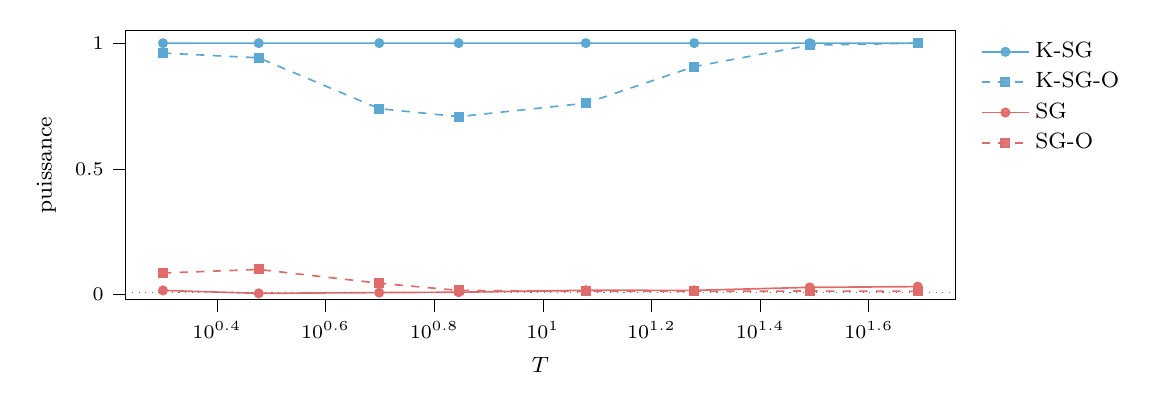
\begin{tikzpicture}

\definecolor{cornflowerblue92168211}{RGB}{92,168,211}
\definecolor{darkgray176}{RGB}{176,176,176}
\definecolor{indianred224107107}{RGB}{224,107,107}
\definecolor{slategray107114128}{RGB}{107,114,128}

\begin{axis}[
height=5cm,
label style={font=\footnotesize},
legend cell align={left},
legend style={
  fill opacity=0.8,
  draw opacity=1,
  text opacity=1,
  at={(1.02,1)},
  anchor=north west,
  draw=none
},
legend style={draw=none, fill=white, fill opacity=0.9, text opacity=1, font=\footnotesize},
log basis x={10},
tick align=outside,
tick label style={font=\scriptsize},
tick pos=left,
title style={font=\footnotesize, yshift=-2pt},
width=\textwidth,
x grid style={darkgray176},
xlabel={\(\displaystyle T\)},
xmin=1.70440065114704, xmax=57.4982178832467,
xmode=log,
xtick style={color=black},
y grid style={darkgray176},
ylabel={puissance},
ymin=-0.02, ymax=1.05,
ytick style={color=black}
]
\addplot [semithick, cornflowerblue92168211, mark=*, mark size=1.5, mark options={solid}]
table {%
2 0.9998
3 1
5 1
7 1
12 1
19 1
31 1
49 1
};
\addlegendentry{K-SG}
\addplot [semithick, cornflowerblue92168211, dashed, mark=square*, mark size=1.5, mark options={solid}]
table {%
2 0.9606
3 0.9416
5 0.7396
7 0.7078
12 0.7612
19 0.9068
31 0.9918
49 0.9998
};
\addlegendentry{K-SG-O}
\addplot [semithick, indianred224107107, mark=*, mark size=1.5, mark options={solid}]
table {%
2 0.017
3 0.0054
5 0.0084
7 0.0098
12 0.0176
19 0.0172
31 0.0292
49 0.0322
};
\addlegendentry{SG}
\addplot [semithick, indianred224107107, dashed, mark=square*, mark size=1.5, mark options={solid}]
table {%
2 0.0862
3 0.1004
5 0.0456
7 0.017
12 0.0134
19 0.013
31 0.0146
49 0.0132
};
\addlegendentry{SG-O}
\addplot [slategray107114128, dotted, forget plot]
table {%
1.70440065114704 0.00999999999999998
57.4982178832467 0.00999999999999998
};
\end{axis}

\end{tikzpicture}

  \provPuissanceKQR[.5cm]
  \caption{Puissance de detection à $\pfa=10^{-2}$ en fonction du nombre de
  dates, en fouillis K-distribue ($\nu=1$), pour les quatre detecteurs: glrt
  hors ligne avec et sans structure de Kronecker, et leurs contreparties
  recursives. Les seuils sont fixes par detecteur et par $\Ntime$ au quantile
  empirique des statistiques sous $\hypothesis_0$, de sorte que toutes les
  courbes se lisent à la meme fausse alarme. $10^3$ tirages.
  \provPuissanceK}
  \label{fig:detection-online-puissance}
\end{figure}

% ============================ FIGURE SUPPLEMENTAIRE ================================
% Pendant gaussien de la precedente. Resultat mesure apres correction des
% detecteurs en ligne (2026-08-25): hors ligne K-SG 0,999 a T=49, recursif
% K-SG-O 0,981; non structure SG 0,272 contre SG-O 0,244. Les recursifs
% rattrapent, mais tard. L'article signale bien que les versions en ligne convergent
% plus lentement en gaussien qu'en K-distribue, mais pas a ce point.
%
% TODO A VERIFIER AVANT D'EN FAIRE UN ARGUMENT. Trois pistes, dans l'ordre:
%  1. avec une texture deterministe egale a 1, le schema recursif continue
%     d'estimer $\vector{\texture}$ librement; le pas $\alpha_0/\Ntime$ met
%     peut-etre beaucoup plus de dates a la ramener vers 1 qu'a l'estimer sous
%     hypothese heterogene;
%  2. les roc de l'article sont a $\Ntime=50$ et montrent les versions en ligne
%     utilisables --- verifier si l'ecart vient du $\pfa$ retenu ici ($10^{-2}$)
%     ou de l'amplitude du changement;
%  3. relancer avec --step-rule armijo pour voir si le comportement tient au pas.
% Tant que ce n'est pas tranche, presenter la figure comme une observation, pas
% comme une propriete du detecteur.
% ====================================================================================
\begin{figure}[htbp]
  \centering
  % This file was created with matplot2tikz v0.5.3.
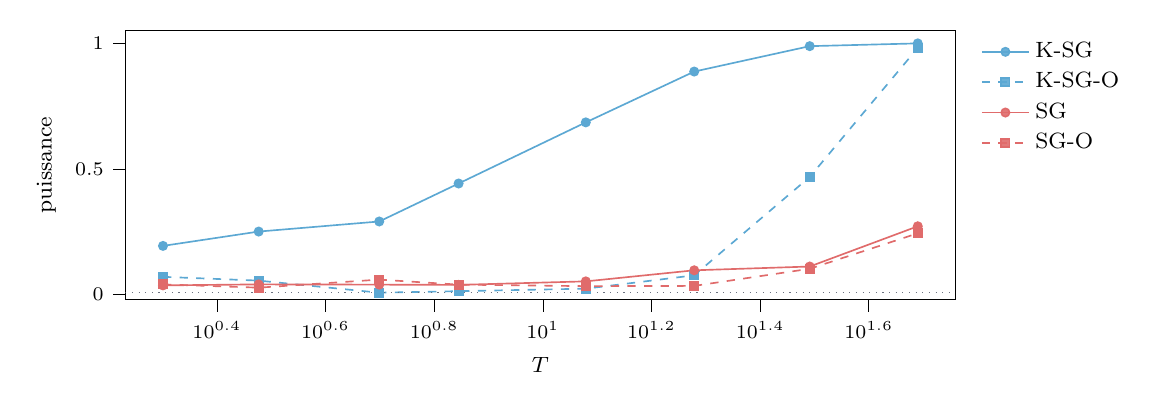
\begin{tikzpicture}

\definecolor{cornflowerblue92168211}{RGB}{92,168,211}
\definecolor{darkgray176}{RGB}{176,176,176}
\definecolor{indianred224107107}{RGB}{224,107,107}
\definecolor{slategray107114128}{RGB}{107,114,128}

\begin{axis}[
height=5cm,
label style={font=\footnotesize},
legend cell align={left},
legend style={
  fill opacity=0.8,
  draw opacity=1,
  text opacity=1,
  at={(1.02,1)},
  anchor=north west,
  draw=none
},
legend style={draw=none, fill=white, fill opacity=0.9, text opacity=1, font=\footnotesize},
log basis x={10},
tick align=outside,
tick label style={font=\scriptsize},
tick pos=left,
title style={font=\footnotesize, yshift=-2pt},
width=\textwidth,
x grid style={darkgray176},
xlabel={\(\displaystyle T\)},
xmin=1.70440065114704, xmax=57.4982178832467,
xmode=log,
xtick style={color=black},
y grid style={darkgray176},
ylabel={puissance},
ymin=-0.02, ymax=1.05,
ytick style={color=black}
]
\addplot [semithick, cornflowerblue92168211, mark=*, mark size=1.5, mark options={solid}]
table {%
2 0.194
3 0.251
5 0.291
7 0.442
12 0.685
19 0.887
31 0.988
49 0.999
};
\addlegendentry{K-SG}
\addplot [semithick, cornflowerblue92168211, dashed, mark=square*, mark size=1.5, mark options={solid}]
table {%
2 0.071
3 0.056
5 0.008
7 0.014
12 0.024
19 0.077
31 0.468
49 0.981
};
\addlegendentry{K-SG-O}
\addplot [semithick, indianred224107107, mark=*, mark size=1.5, mark options={solid}]
table {%
2 0.037
3 0.041
5 0.04
7 0.039
12 0.053
19 0.097
31 0.112
49 0.272
};
\addlegendentry{SG}
\addplot [semithick, indianred224107107, dashed, mark=square*, mark size=1.5, mark options={solid}]
table {%
2 0.041
3 0.028
5 0.06
7 0.04
12 0.034
19 0.035
31 0.103
49 0.244
};
\addlegendentry{SG-O}
\addplot [slategray107114128, dotted, forget plot]
table {%
1.70440065114704 0.00999999999999998
57.4982178832467 0.00999999999999998
};
\end{axis}

\end{tikzpicture}

  \provPuissanceGaussienQR[.5cm]
  \caption{Meme experience que la \cref{fig:detection-online-puissance}, mais en
  fouillis gaussien ($\texture_\iobs=1$). Les deux detecteurs recursifs
  rejoignent leur contrepartie hors ligne, mais bien plus tard qu'en
  environnement heterogene: la ou le Kronecker recursif collait au hors ligne
  des $\Ntime=2$ en fouillis K, il lui faut ici toute la serie pour le
  rattraper. Le schema stochastique tire donc parti de l'heterogeneite qu'il
  est cense combattre. $10^3$ tirages. \provPuissanceGaussien}
  \label{fig:detection-online-puissance-gaussien}
\end{figure}

% Les benchmarks temps/memoire hors ligne vs en ligne completent l'analyse de
% complexite: c'est le versant pratique de l'argument.
\wipfig{Temps de calcul en ligne}{Temps de mise à jour de la carte de détection à l'arrivée d'une nouvelle image en fonction du nombre de dates $\Ntime$, pour les quatre détecteurs (glrt hors ligne avec et sans structure de Kronecker, et leurs versions récursives), sur CPU et GPU, mêmes conventions que la \cref{fig:benchmark_sar_offline}. Attendu: croissance linéaire en $\Ntime$ hors ligne, palier constant en ligne. Expérience: à câbler à partir des benchmarks existants.}

% Cartes de detection sur donnees UAVSAR reelles: les donnees sont
% telechargeables (script download_sar.sh). La repetition de la serie
% (T=68, 340, 680) est outillee: load_sits accepte --repeat-times, avec un
% rebond palindrome plutot que la concatenation brute de l'article --- a
% signaler en legende, c'est une difference assumee qui evite une discontinuite
% a la couture.
% ABANDONNE: les courbes roc hors ligne vs en ligne sur donnees simulees font
% doublon avec la figure mse et les cartes reelles.
\wipfig{Cartes UAVSAR hors ligne et en ligne}{Série SDelta\_28518\_02 (segment 1, $200\times200$ pixels, $\vdim=12$ après ondelettes, fenêtre $7\times7$). Quatre cartes (glrt gaussien à échelle et sa version Kronecker, hors ligne et en ligne) pour $\Ntime=68$, puis la série répétée en palindrome jusqu'à $\Ntime=340$ et $680$. Message attendu: l'écart entre version en ligne et hors ligne se referme quand $\Ntime$ croît, plus vite avec la structure de Kronecker.}

\wip{Lecture des résultats sur données réelles}{Deux ou trois phrases une fois les cartes produites: en l'absence de vérité terrain, on ne juge que la proximité entre versions en ligne et hors ligne; dire à partir de quel $\Ntime$ elles se confondent, et si la structure accélère ce rapprochement comme sur données simulées.}

\FloatBarrier
\section{Bilan}
\label{sec:detection-synthese}

\wip{Bilan ch. détection: la science}{Quatre points: ce qui circule entre les deux moitiés du chapitre (la même estimation de matrice de forme, contrainte tantôt statistiquement tantôt géométriquement); l'axe sélectivité/robustesse comme grille de lecture; les points ouverts assumés (unicité, seuils en forme close, aucun travail ne combine en-ligne et structure); la transition vers le chapitre SPDnet. Environ 1 page.}

\wip{Bilan ch. détection: les six mouvements}{À placer AVANT la transition. Nommer les personnes avec les dates --- aucun nom n'apparaît aujourd'hui dans ce chapitre; l'application qui a unifié le travail; ce qui a été construit, en clair; pointer les articles reproduits par leur folio (\texttt{\textbackslash paperpage\{JOE24\}} p.~\paperpage{JOE24}, JOE26 p.~\pageref{paper:JOE26}, SP24 p.~\pageref{paper:SP24}); dire que le travail excède les articles joints; dire où cela continue. Puis 3 ou 4 perspectives propres au chapitre en paragraphes à titre courant.}

% ============================ TODO texte (~1 page) =================================
% Quatre choses a dire, dans cet ordre:
%
%  1. CE QUI CIRCULE ENTRE LES DEUX MOITIES. Le meme objet --- l'estimation au
%     sens du maximum de vraisemblance de la matrice de forme d'un modele
%     gaussien a echelle --- traverse tout le chapitre, contraint tantot par une
%     structure statistique (deux antennes, Kronecker, Toeplitz, sous-espace),
%     tantot par une structure geometrique (recursion sur la variete). Dans les
%     deux cas c'est la contrainte qui rend le probleme faisable au $\Nobs$ dont
%     on dispose reellement, et non un raffinement de performance.
%
%  2. L'AXE SELECTIVITE/ROBUSTESSE comme grille de lecture, pas comme
%     catalogue: le test de Rao (\cref{prop:detection-mills-rao}) et les
%     detecteurs par sous-espace (\cref{prop:detection-fls-anmf-sousespace})
%     sont les deux poles d'un meme continuum, et le glrt s'y situe entre les
%     deux. Renvoyer aux deux figures tracees sur les memes axes.
%
%  3. LES POINTS OUVERTS, a assumer explicitement --- c'est ce qu'un jury
%     d'hdr attend:
%       - l'unicite de l'estimateur a deux textures \cref{eq:detection-mills-tyler}
%         n'est etablie que numeriquement;
%       - les seuils en forme close manquent pour les detecteurs structures
%         adaptatifs, d'ou le recours systematique a la simulation;
%       - surtout: aucun des trois travaux ne combine les deux leviers, c'est-a-dire
%         l'estimation *en ligne* d'une covariance *structuree sous contrainte*
%         (Toeplitz), ou la contrainte n'est justement pas compatible avec la
%         geometrie du cone. C'est la perspective la plus naturelle du chapitre.
%
%  4. TRANSITION vers le \cref{ch:learning} --- ATTENTION, ce n'est plus le
%     \cref{ch:spdnet} qui suit. Le point de bascule a formuler est celui-ci:
%     dans tout ce chapitre, le modele fait DEUX choses a la fois --- il
%     fournit l'estimateur ET il fournit le critere qui juge la decision (la
%     loi sous $\hypothesis_0$, le seuil, la propriete cfar). Que la dispersion
%     y soit parametre de nuisance ou parametre teste n'y change rien: c'est
%     meme le seul point commun des deux archetypes de la
%     \cref{subsec:detection-archetypes}. Le chapitre suivant est celui ou la
%     seconde de ces deux fonctions tombe, et ou le modele doit se contenter de
%     la premiere. NE PAS annoncer la transition en termes de regime
%     dimensionnel: ce n'est pas ce qui change.
% ====================================================================================

% ============ TODO texte (~1 page) --- LES SIX MOUVEMENTS DE CHATELAIN =============
% A INSERER AVANT le point 4 ci-dessus (la transition doit rester la derniere
% chose du chapitre). Le modele est le \S1.6 de Chatelain, dont chaque bilan de
% chapitre enchaine six mouvements. Les points 1 a 3 ci-dessus couvrent la
% science; ce qui manque est tout le reste, et c'est ce qu'un jury lit.
%
%  (a) NOMMER LES PERSONNES, AVEC LES DATES. « developpes dans le cadre des
%      theses de X (soutenue en 20..) et de Y (soutenue en 20..) ». Ici: les
%      collaborations sonar, et le volet detection de changements RSO. Preciser
%      qui a fait quoi. AUJOURD'HUI AUCUN NOM N'APPARAIT DANS CE CHAPITRE:
%      l'encadrement est entierement relegue au \cref{ch:cv}, ce qui est le
%      defaut le plus couteux du memoire en l'etat.
%
%  (b) L'APPLICATION QUI A UNIFIE LE TRAVAIL, en une phrase. Le fil n'est pas
%      « la detection robuste » en general mais trois capteurs qui imposent le
%      meme compromis.
%
%  (c) CE QUI A ETE CONSTRUIT, EN CLAIR. Pas d'equations dans ce paragraphe.
%
%  (d) POINTER LES ARTICLES REPRODUITS AVEC LEUR FOLIO, dans le fil du texte.
%      La macro existe desormais: « annexe p.~\paperpage{JOE24} » (p. 133),
%      \paperpage{JOE26} (p. 147), \paperpage{SP24} (p. 163). C'est ce qui
%      soude les pdf joints a l'argumentation au lieu d'en faire une annexe ou
%      personne n'entre.
%
%  (e) DIRE QUE LE TRAVAIL EXCEDE LES ARTICLES JOINTS. « Ce travail ne se
%      limite pas aux trois articles reproduits ci-apres », puis citer le
%      reste (dont \fullcite{GRETSI23a}). Cela pose la selection comme un choix
%      editorial et non comme un inventaire.
%
%  (f) DIRE OU CELA CONTINUE MAINTENANT: these en cours, collaboration en
%      cours, nommement.
%
% Puis 3 ou 4 PERSPECTIVES PROPRES AU CHAPITRE, en paragraphes a titre courant
% gras (« \paragraph{Titre.} »), comme Chatelain. Elles allegent d'autant le
% \cref{ch:perspectives}.
% ====================================================================================

% ============================ TODO decision ========================================
% Deux points de mise en forme restes en suspens:
%  (a) PREUVES. Mon avis: la derivation du test de Rao
%      (\cref{prop:detection-mills-rao}) en annexe de chapitre, car c'est la
%      contribution la moins accessible et celle qu'un lecteur voudra verifier;
%      les autres derivations renvoyees aux pdf joints. Prevoir dans ce cas une
%      section « Complements » en fin de chapitre.
%  (b) PDF JOINTS. FAIT: pdfpages et les macros \joinedpapers/\joinedpaper sont
%      dans classicthesis-config.tex, les trois articles sont inclus en fin de
%      fichier. Reste \fullcite{GRETSI23a}, annonce dans l'encadre d'ouverture
%      mais sans pdf dans papers/.
% ====================================================================================

% ====================================================================================
% Articles reproduits. L'ordre suit celui dans lequel le chapitre les mobilise:
% Mills Cross (sections 1-2), FLS multi-pings (section 3), changement RSO
% (section 4). \fullcite{GRETSI23a}, annonce dans l'encadre d'ouverture, n'a pas
% de pdf dans papers/ : soit l'ajouter, soit le retirer de l'encadre.
% ====================================================================================
\joinedpapers{%
  Les versions publiées des travaux dont rend compte ce chapitre sont reproduites
  ci-après, dans l'ordre où le chapitre les mobilise.

  \joinedpaper[JOE24]{\citeauthor{JOE24}, \citetitle{JOE24}}{papers/DEMR2023-031.pdf}
  \joinedpaper[JOE26]{\citeauthor{JOE26}, \citetitle{JOE26}}{papers/Robust_Multiping_Forward-Looking_Sonar_Coherent_Detection.pdf}
  \joinedpaper[SP24]{\citeauthor{SP24}, \citetitle{SP24}}{papers/1-s2.0-S0165168424002081-main.pdf}
}
